\chapter{Basic Usage}





In interactive code examples that follow, it will be assumed that all items in the mpFormulaPy
namespace have been imported:

\lstset{language={Python}}
\begin{lstlisting}
>>> from mpFormulaPy import *
\end{lstlisting}

Importing everything can be convenient, especially when using mpFormulaPy interactively, but be careful when mixing mpFormulaPy with other libraries! To avoid inadvertently overriding other functions or objects, explicitly import only the needed objects, or use the mpFormulaPy. or mp.namespaces:


\lstset{language={Python}}
\begin{lstlisting}
from mpFormulaPy import sin, cos
sin(1), cos(1)
import mpFormulaPy
mpFormulaPy.sin(1), mpFormulaPy.cos(1)
from mpFormulaPy import mp # mp context object -- to be explained
mp.sin(1), mp.cos(1)>>> from mpFormulaPy import *
\end{lstlisting}



\section{Number types}
Mpmath provides the following numerical types:

\begin{verbatim}
Class Description
mpf Real float
mpc Complex float
matrix Matrix
\end{verbatim}


Currently missing: decimals. The MPD reference is \cite{mpd_2012}


The following section will provide a very short introduction to the types mpf and mpc. Intervals and matrices are described further in the documentation chapters on interval arithmetic and matrices / linear algebra.

\vpara
The mpf type is analogous to Python's built-in float. It holds a real number or one of the special values inf (positive infinity), -inf (negative infinity) and nan (not-a-number, indicating an indeterminate result). You can create mpf instances from strings, integers, floats, and
other mpf instances:

\lstset{language={Python}}
\begin{lstlisting}
>>> mpf(4)
mpf('4.0')
>>> mpf(2.5)
mpf('2.5')
>>> mpf("1.25e6")
mpf('1250000.0')
>>> mpf(mpf(2))
mpf('2.0')
>>> mpf("inf")
mpf('+inf')
\end{lstlisting}


The mpc type represents a complex number in rectangular form as a pair of mpf instances. It can be constructed from a Python complex, a real number, or a pair of real numbers:

\lstset{language={Python}}
\begin{lstlisting}
>>> mpc(2,3)
mpc(real='2.0', imag='3.0')
>>> mpc(complex(2,3)).imag
mpf('3.0')
\end{lstlisting}


You can mix mpf and mpc instances with each other and with Python numbers:

\lstset{language={Python}}
\begin{lstlisting}
>>> mpf(3) + 2*mpf('2.5') + 1.0
mpf('9.0')
>>> mp.dps = 15 # Set precision (see below)
>>> mpc(1j)**0.5
mpc(real='0.70710678118654757', imag='0.70710678118654757')
\end{lstlisting}


\subsection{Setting the precision} 

Mpmath uses a global working precision; it does not keep track of the precision or accuracy of individual numbers. Performing an arithmetic operation or calling mpf() rounds the result to the current working precision. The working precision is controlled by a context object called mp, which has the following default states:

\lstset{language={Python}}
\begin{lstlisting}
>>> from mpFormulaPy import *
>>> mp.dps
25
>>> mp.prec
86
>>> mp.trap_complex
False
>>>
\end{lstlisting}


The term prec denotes the binary precision (measured in bits) while dps (short for decimal places) is the decimal precision. Binary and decimal precision are related roughly according to the formula prec = 3.33*dps. For example, it takes a precision of roughly 333 bits to hold an approximation of pi that is accurate to 100 decimal places (actually slightly more than 333 bits is used).

\vpara
Changing either precision property of the mp object automatically updates the other; usually you just want to change the dps value:

\lstset{language={Python}}
\begin{lstlisting}
>>> mp.dps = 100
>>> mp.dps
100
>>> mp.prec
336
\end{lstlisting}


When the precision has been set, all mpf operations are carried out at that precision:

\lstset{language={Python}}
\begin{lstlisting}
>>> mp.dps = 50
>>> mpf(1) / 6
mpf('0.16666666666666666666666666666666666666666666666666656')
>>> mp.dps = 25
>>> mpf(2) ** mpf('0.5')
mpf('1.414213562373095048801688713')
\end{lstlisting}

The precision of complex arithmetic is also controlled by the mp object:

\lstset{language={Python}}
\begin{lstlisting}
>>> mp.dps = 10
>>> mpc(1,2) / 3
mpc(real='0.3333333333321', imag='0.6666666666642')
\end{lstlisting}


There is no restriction on the magnitude of numbers. An mpf can for example hold an approximation of a large Mersenne prime:

\lstset{language={Python}}
\begin{lstlisting}
>>> mp.dps = 15
>>> print mpf(2)**32582657 - 1
1.24575026015369e+9808357
\end{lstlisting}


Or why not 1 googolplex:

\lstset{language={Python}}
\begin{lstlisting}
>>> print mpf(10) ** (10**100)
1.0e+100000000000000000000000000000000000000000000000000...
\end{lstlisting}


The (binary) exponent is stored exactly and is independent of the precision.


\subsection{Temporarily changing the precision}  

It is often useful to change the precision during only part of a calculation. A way to temporarily increase the precision and then restore it is as follows:

\lstset{language={Python}}
\begin{lstlisting}
>>> mp.prec += 2
>>> # do_something()
>>> mp.prec -= 2
\end{lstlisting}


As of Python 2.5, the with statement along with the mpFormulaPy functions workprec, workdps, extraprec and extradps can be used to temporarily change precision in a more safe manner:

\lstset{language={Python}}
\begin{lstlisting}
>>> from __future__ import with_statement
>>> with workdps(20):
... print mpf(1)/7
... with extradps(10):
... print mpf(1)/7
...
0.14285714285714285714
0.142857142857142857142857142857
>>> mp.dps
15
\end{lstlisting}


The with statement ensures that the precision gets reset when exiting the block, even in the case that an exception is raised. (The effect of the with statement can be emulated in Python 2.4 by using a try/finally block.)

The workprec family of functions can also be used as function decorators:

\lstset{language={Python}}
\begin{lstlisting}
>>> @workdps(6)
... def f():
... return mpf(1)/3
...
>>> f()
mpf('0.33333331346511841')
\end{lstlisting}


Some functions accept the prec and dps keyword arguments and this will override the global working precision. Note that this will not affect the precision at which the result is printed, so to get all digits, you must either use increase precision afterward when printing or use nstr/nprint:

\lstset{language={Python}}
\begin{lstlisting}
>>> mp.dps = 15
>>> print exp(1)
2.71828182845905
>>> print exp(1, dps=50) # Extra digits won't be printed
2.71828182845905
>>> nprint(exp(1, dps=50), 50)
2.7182818284590452353602874713526624977572470937
\end{lstlisting}


Finally, instead of using the global context object mp, you can create custom contexts and work with methods of those instances instead of global functions. The working precision will be local to each context object:

\lstset{language={Python}}
\begin{lstlisting}
>>> mp2 = mp.clone()
>>> mp.dps = 10
>>> mp2.dps = 20
>>> print mp.mpf(1) / 3
0.3333333333
>>> print mp2.mpf(1) / 3
0.33333333333333333333
\end{lstlisting}


Note: the ability to create multiple contexts is a new feature that is only partially implemented. Not all mpFormulaPy functions are yet available as context-local methods. In the present version, you are likely to encounter bugs if you try mixing different contexts.


\subsection{Providing correct input}  

Note that when creating a new mpf, the value will at most be as accurate as the input. Be careful when mixing mpFormulaPy numbers with Python floats. When working at high precision, fractional mpf values should be created from strings or integers:

\lstset{language={Python}}
\begin{lstlisting}
>>> mp.dps = 30
>>> mpf(10.9) # bad
mpf('10.9000000000000003552713678800501')
>>> mpf('10.9') # good
mpf('10.8999999999999999999999999999997')
>>> mpf(109) / mpf(10) # also good
mpf('10.8999999999999999999999999999997')
>>> mp.dps = 15
\end{lstlisting}


(Binary fractions such as 0.5, 1.5, 0.75, 0.125, etc, are generally safe as input, however, since those can be represented exactly by Python floats.)


\subsection{Printing}  

By default, the repr() of a number includes its type signature. This way eval can be used to recreate a number from its string representation:

\lstset{language={Python}}
\begin{lstlisting}
>>> eval(repr(mpf(2.5)))
mpf('2.5')
\end{lstlisting}


Prettier output can be obtained by using str() or print, which hide the mpf and mpc signatures and also suppress rounding artifacts in the last few digits:

\lstset{language={Python}}
\begin{lstlisting}
>>> mpf("3.14159")
mpf('3.1415899999999999')
>>> print mpf("3.14159")
3.14159
>>> print mpc(1j)**0.5
(0.707106781186548 + 0.707106781186548j)
\end{lstlisting}


Setting the mp.pretty option will use the str()-style output for repr() as well:

\lstset{language={Python}}
\begin{lstlisting}
>>> mp.pretty = True
>>> mpf(0.6)
0.6
>>> mp.pretty = False
>>> mpf(0.6)
mpf('0.59999999999999998')
\end{lstlisting}


The number of digits with which numbers are printed by default is determined by the working precision. To specify the number of digits to show without changing the working precision, use mpFormulaPy.nstr() and mpFormulaPy.nprint():

\lstset{language={Python}}
\begin{lstlisting}
>>> a = mpf(1) / 6
>>> a
mpf('0.16666666666666666')
>>> nstr(a, 8)
'0.16666667'
>>> nprint(a, 8)
0.16666667
>>> nstr(a, 50)
'0.16666666666666665741480812812369549646973609924316'
\end{lstlisting}














\subsection{Contexts}  

High-level code in mpFormulaPy is implemented as methods on a 'context object'. The context implements arithmetic, type conversions and other fundamental operations. The context also holds settings such as precision, and stores cache data. A few different contexts (with a
mostly compatible interface) are provided so that the high-level algorithms can be used with different implementations of the underlying arithmetic, allowing different features and speed/accuracy tradeoffs. Currently, mpFormulaPy provides the following contexts:

\vpara
Arbitrary-precision arithmetic (mp)

A faster Cython-based version of mp (used by default in Sage, and currently only available there)

Arbitrary-precision interval arithmetic (iv)

Double-precision arithmetic using Python's builtin float and complex types (fp)

\vpara
Most global functions in the global mpFormulaPy namespace are actually methods of the mp context. This fact is usually transparent to the user, but sometimes shows up in the form of an initial parameter called 'ctx' visible in the help for the function:

\lstset{language={Python}}
\begin{lstlisting}
>>> import mpFormulaPy
>>> help(mpFormulaPy.fsum)
Help on method fsum in module mpFormulaPy.ctx_mp_python:
fsum(ctx, terms, absolute=False, squared=False) method of mpFormulaPy.ctx_mp.MPContext ins
Calculates a sum containing a finite number of terms (for infinite
series, see :func:`~mpFormulaPy.nsum`). The terms will be converted to
...
\end{lstlisting}



The following operations are equivalent:

\lstset{language={Python}}
\begin{lstlisting}
>>> mpFormulaPy.mp.dps = 15; mpFormulaPy.mp.pretty = False
>>> mpFormulaPy.fsum([1,2,3])
mpf('6.0')
>>> mpFormulaPy.mp.fsum([1,2,3])
mpf('6.0')
\end{lstlisting}


The corresponding operation using the fp context:

\lstset{language={Python}}
\begin{lstlisting}
>>> mpFormulaPy.fp.fsum([1,2,3])
6.0
\end{lstlisting}


\subsection{Common interface}  

ctx.mpf creates a real number:

\lstset{language={Python}}
\begin{lstlisting}
>>> from mpFormulaPy import mp, fp
>>> mp.mpf(3)
mpf('3.0')
>>> fp.mpf(3)
3.0
\end{lstlisting}


ctx.mpc creates a complex number:

\lstset{language={Python}}
\begin{lstlisting}
>>> mp.mpc(2,3)
mpc(real='2.0', imag='3.0')
>>> fp.mpc(2,3)
(2+3j)
\end{lstlisting}


ctx.matrix creates a matrix:

\lstset{language={Python}}
\begin{lstlisting}
>>> mp.matrix([[1,0],[0,1]])
matrix(
[['1.0', '0.0'],
['0.0', '1.0']])
>>> _[0,0]
mpf('1.0')
>>> fp.matrix([[1,0],[0,1]])
matrix(
[['1.0', '0.0'],
['0.0', '1.0']])
>>> _[0,0]
1.0
\end{lstlisting}


ctx.prec holds the current precision (in bits):

\lstset{language={Python}}
\begin{lstlisting}
>>> mp.prec
53
>>> fp.prec
53
\end{lstlisting}


ctx.dps holds the current precision (in digits):

\lstset{language={Python}}
\begin{lstlisting}
>>> mp.dps
15
>>> fp.dps
15
\end{lstlisting}


ctx.pretty controls whether objects should be pretty-printed automatically by repr(). Prettyprinting for mp numbers is disabled by default so that they can clearly be distinguished from Python numbers and so that eval(repr(x)) == x works:

\lstset{language={Python}}
\begin{lstlisting}
>>> mp.mpf(3)
mpf('3.0')
>>> mpf = mp.mpf
>>> eval(repr(mp.mpf(3)))
mpf('3.0')
>>> mp.pretty = True
>>> mp.mpf(3)
3.0
>>> fp.matrix([[1,0],[0,1]])
matrix(
[['1.0', '0.0'],
['0.0', '1.0']])
>>> fp.pretty = True
>>> fp.matrix([[1,0],[0,1]])
[1.0 0.0]
[0.0 1.0]
>>> fp.pretty = False
>>> mp.pretty = False
\end{lstlisting}



\subsection{Arbitrary-precision floating-point (mp)}  

The mp context is what most users probably want to use most of the time, as it supports the most functions, is most well-tested, and is implemented with a high level of optimization. Nearly all examples in this documentation use mp functions.

See Basic usage for a description of basic usage.


\subsection{Arbitrary-precision interval arithmetic (iv)}  

The iv.mpf type represents a closed interval $[a,]$; that is, the set $\{x: a \leq x \leq b\}$, where $a$ and $b $ are arbitrary-precision floating-point values, possibly $\pm\infty$. The iv.mpc type represents a rectangular complex interval $[a,b] + [c,d]i$; that is, the set $\{z=x+iy: a \leq x \leq b \wedge c \leq y \leq d\}$.

\vpara
Interval arithmetic provides rigorous error tracking. If  $f$ is a mathematical function and $\hat{f}$ is its interval arithmetic version, then the basic guarantee of interval arithmetic is that $f(v) \subseteq \hat{f}(v)$ for any input interval $v$. Put differently, if an interval represents the known uncertainty for a fixed number, any sequence of interval operations will produce an interval that contains what would be the result of applying the same sequence of operations to the exact number. The principal drawbacks of interval arithmetic are speed (iv arithmetic is typically at least two times slower than mp arithmetic) and that it sometimes provides far too pessimistic bounds.

\vpara
Note: The support for interval arithmetic in mpFormulaPy is still experimental, and many functions do not yet properly support intervals. Please use this feature with caution.

\vpara
Intervals can be created from single numbers (treated as zero-width intervals) or pairs of endpoint numbers. Strings are treated as exact decimal numbers. Note that a Python float like 0.1 generally does not represent the same number as its literal; use '0.1' instead:

\lstset{language={Python}}
\begin{lstlisting}
>>> from mpFormulaPy import iv
>>> iv.dps = 15; iv.pretty = False
>>> iv.mpf(3)
mpi('3.0', '3.0')
>>> print iv.mpf(3)
[3.0, 3.0]
>>> iv.pretty = True
>>> iv.mpf([2,3])
[2.0, 3.0]
>>> iv.mpf(0.1) # probably not intended
[0.10000000000000000555, 0.10000000000000000555]
>>> iv.mpf('0.1') # good, gives a containing interval
[0.099999999999999991673, 0.10000000000000000555]
>>> iv.mpf(['0.1', '0.2'])
[0.099999999999999991673, 0.2000000000000000111]
\end{lstlisting}


The fact that '0.1' results in an interval of nonzero width indicates that 1/10 cannot be represented using binary floating-point numbers at this precision level (in fact, it cannot be represented exactly at any precision).

\vpara
Intervals may be infinite or half-infinite:

\lstset{language={Python}}
\begin{lstlisting}
>>> print 1 / iv.mpf([2, 'inf'])
[0.0, 0.5]
\end{lstlisting}


The equality testing operators $==$ and $!=$ check whether their operands are identical as intervals; that is, have the same endpoints. The ordering operators $<$,  $<=$,  $>$ and $>=$ permit inequality testing using triple-valued logic: a guaranteed inequality returns True or False while an indeterminate inequality returns None:

\lstset{language={Python}}
\begin{lstlisting}
>>> iv.mpf([1,2]) == iv.mpf([1,2])
True
>>> iv.mpf([1,2]) != iv.mpf([1,2])
False
>>> iv.mpf([1,2]) <= 2
True
>>> iv.mpf([1,2]) > 0
True
>>> iv.mpf([1,2]) < 1
False
>>> iv.mpf([1,2]) < 2 # returns None
>>> iv.mpf([2,2]) < 2
False
>>> iv.mpf([1,2]) <= iv.mpf([2,3])
True
>>> iv.mpf([1,2]) < iv.mpf([2,3]) # returns None
>>> iv.mpf([1,2]) < iv.mpf([-1,0])
False
\end{lstlisting}


The in operator tests whether a number or interval is contained in another interval:

\lstset{language={Python}}
\begin{lstlisting}
>>> iv.mpf([0,2]) in iv.mpf([0,10])
True
>>> 3 in iv.mpf(['-inf', 0])
False
\end{lstlisting}


Intervals have the properties .a, .b (endpoints), .mid, and .delta (width):

\lstset{language={Python}}
\begin{lstlisting}
>>> x = iv.mpf([2, 5])
>>> x.a
[2.0, 2.0]
>>> x.b
[5.0, 5.0]
>>> x.mid
[3.5, 3.5]
>>> x.delta
[3.0, 3.0]
\end{lstlisting}


Some transcendental functions are supported:

\lstset{language={Python}}
\begin{lstlisting}
>>> iv.dps = 15
>>> mp.dps = 15
>>> iv.mpf([0.5,1.5]) ** iv.mpf([0.5, 1.5])
[0.35355339059327373086, 1.837117307087383633]
>>> iv.exp(0)
[1.0, 1.0]
>>> iv.exp(['-inf','inf'])
[0.0, +inf]
>>>
>>> iv.exp(['-inf',0])
[0.0, 1.0]
>>> iv.exp([0,'inf'])
[1.0, +inf]
>>> iv.exp([0,1])
[1.0, 2.7182818284590455349]
>>>
>>> iv.log(1)
[0.0, 0.0]
>>> iv.log([0,1])
[-inf, 0.0]
>>> iv.log([0,'inf'])
[-inf, +inf]
>>> iv.log(2)
[0.69314718055994528623, 0.69314718055994539725]
>>>
>>> iv.sin([100,'inf'])
[-1.0, 1.0]
>>> iv.cos(['-0.1','0.1'])
[0.99500416527802570954, 1.0]
\end{lstlisting}


Interval arithmetic is useful for proving inequalities involving irrational numbers. Naive use of mp arithmetic may result in wrong conclusions, such as the following:

\lstset{language={Python}}
\begin{lstlisting}
>>> mp.dps = 25
>>> x = mp.exp(mp.pi*mp.sqrt(163))
>>> y = mp.mpf(640320**3+744)
>>> print x
262537412640768744.0000001
>>> print y
262537412640768744.0
>>> x > y
True
\end{lstlisting}


But the correct result is $e^{\pi\sqrt{163}} < 262537412640768744$, as can be seen by increasing the precision:

\lstset{language={Python}}
\begin{lstlisting}
>>> mp.dps = 50
>>> print mp.exp(mp.pi*mp.sqrt(163))
262537412640768743.99999999999925007259719818568888
\end{lstlisting}


With interval arithmetic, the comparison returns None until the precision is large enough for $x-y$ to have a definite sign:

\lstset{language={Python}}
\begin{lstlisting}
>>> iv.dps = 15
>>> iv.exp(iv.pi*iv.sqrt(163)) > (640320**3+744)
>>> iv.dps = 30
>>> iv.exp(iv.pi*iv.sqrt(163)) > (640320**3+744)
>>> iv.dps = 60
>>> iv.exp(iv.pi*iv.sqrt(163)) > (640320**3+744)
False
>>> iv.dps = 15
\end{lstlisting}


\subsection{Fast low-precision arithmetic (fp)}  

Although mpFormulaPy is generally designed for arbitrary-precision arithmetic, many of the high-level algorithms work perfectly well with ordinary Python float and complex numbers, which use hardware double precision (on most systems, this corresponds to 53 bits of precision). 

Whereas the global functions (which are methods of the mp object) always
convert inputs to mpFormulaPy numbers, the fp object instead converts them to float or complex, and in some cases employs basic functions optimized for double precision. When large amounts of function evaluations (numerical integration, plotting, etc) are required, and when
fp arithmetic provides sufficient accuracy, this can give a significant speedup over mp arithmetic.

\vpara
To take advantage of this feature, simply use the fp prefix, i.e. write fp.func instead of func or mp.func:

\lstset{language={Python}}
\begin{lstlisting}
>>> u = fp.erfc(2.5)
>>> print u
0.000406952017445
>>> type(u)
<type 'float'>
>>> mp.dps = 15
>>> print mp.erfc(2.5)
0.000406952017444959
>>> fp.matrix([[1,2],[3,4]]) ** 2
matrix(
[['7.0', '10.0'],
['15.0', '22.0']])
>>>
>>> type(_[0,0])
<type 'float'>
>>> print fp.quad(fp.sin, [0, fp.pi]) # numerical integration
2.0
\end{lstlisting}


The fp context wraps Python's math and cmath modules for elementary functions. It supports both real and complex numbers and automatically generates complex results for real inputs (math raises an exception):

\lstset{language={Python}}
\begin{lstlisting}
>>> fp.sqrt(5)
2.23606797749979
>>> fp.sqrt(-5)
2.23606797749979j
>>> fp.sin(10)
-0.5440211108893698
>>> fp.power(-1, 0.25)
(0.7071067811865476+0.7071067811865475j)
>>> (-1) ** 0.25
Traceback (most recent call last):
...
ValueError: negative number cannot be raised to a fractional power
\end{lstlisting}


The prec and dps attributes can be changed (for interface compatibility with the mp context) but this has no effect:

\lstset{language={Python}}
\begin{lstlisting}
>>> fp.prec
53
>>> fp.dps
15
>>> fp.prec = 80
>>> fp.prec
53
>>> fp.dps
15
\end{lstlisting}


Due to intermediate rounding and cancellation errors, results computed with fp arithmetic may be much less accurate than those computed with mp using an equivalent precision (mp.prec = 53), since the latter often uses increased internal precision. The accuracy is highly problem-dependent: for some functions, fp almost always gives 14-15 correct digits; for others, results can be accurate to only 2-3 digits or even completely wrong. The recommended use for fp is therefore to speed up large-scale computations where accuracy can be verified in advance on a subset of the input set, or where results can be verified afterwards.




\newpage
\section{Precision and representation issues}

Most of the time, using mpFormulaPy is simply a matter of setting the desired precision and entering a formula. For verification purposes, a quite (but not always!) reliable technique is to calculate the same thing a second time at a higher precision and verifying that the results
agree.

\vpara
To perform more advanced calculations, it is important to have some understanding of how mpFormulaPy works internally and what the possible sources of error are. This section gives an overview of arbitrary-precision binary floating-point arithmetic and some concepts from
numerical analysis.

\vpara
The following concepts are important to understand:

\vpara
The main sources of numerical errors are rounding and cancellation, which are due to the use of finite-precision arithmetic, and truncation or approximation errors, which are due to approximating infinite sequences or continuous functions by a finite number of samples.

\vpara
Errors propagate between calculations. A small error in the input may result in a large error in the output.

\vpara
Most numerical algorithms for complex problems (e.g. integrals, derivatives) give wrong answers for sufficiently ill-behaved input. Sometimes virtually the only way to get a wrong answer is to design some very contrived input, but at other times the chance of accidentally obtaining a wrong result even for reasonable-looking input is quite high.

\vpara
Like any complex numerical software, mpFormulaPy has implementation bugs. You should be reasonably suspicious about any results computed by mpFormulaPy, even those it claims to be able to compute correctly! If possible, verify results analytically, try different algorithms, and cross-compare with other software.



\subsection{Precision, error and tolerance}

The following terms are common in this documentation:

\vpara
Precision (or working precision) is the precision at which floating-point arithmetic operations are performed.

\vpara
Error is the difference between a computed approximation and the exact result.

\vpara
Accuracy is the inverse of error.

\vpara
Tolerance is the maximum error (or minimum accuracy) desired in a result.

\vpara
Error and accuracy can be measured either directly, or logarithmically in bits or digits. Specifically, if a $\hat{y}$ is an approximation for $y$, then

\vpara
(Direct) absolute error = $|\hat{y} - y|$

(Direct) relative error = $|\hat{y} - y||y|^{-1}$

(Direct) absolute accuracy = $|\hat{y} - y|^{-1}$

(Direct) relative accuracy = $|\hat{y} - y|^{-1}|y|$

(Logarithmic) absolute error = $\log_b|\hat{y} - y|$

(Logarithmic) relative error = $\log_b|\hat{y} - y| - \log_b|y|$

(Logarithmic) absolute accuracy = $-\log_b|\hat{y} - y|$

(Logarithmic) relative accuracy =$-\log_b|\hat{y} - y| - \log_b|y|$

\vpara
where $b=2$ and $b=10$ for bits and digits respectively. Note that:

\vpara
The logarithmic error roughly equals the position of the first incorrect bit or digit.

The logarithmic accuracy roughly equals the number of correct bits or digits in the result.

\vpara
These definitions also hold for complex numbers, using $|a+bi|=\sqrt{a^2+b^2}$.

Full accuracy means that the accuracy of a result at least equals prec-1, i.e. it is correct except possibly for the last bit.




\subsection{Representation of numbers}

Mpmath uses binary arithmetic. A binary floating-point number is a number of the form $man \times 2^{exp}$ where both man (the mantissa) and exp (the exponent) are integers. Some examples of floating-point numbers are given in the following table.

\vpara
\begin{verbatim}
Number Mantissa Exponent
3 3 0
10 5 1
-16 -1 4
1.25 5 -2
\end{verbatim}


\vpara
The representation as defined so far is not unique; one can always multiply the mantissa by 2 and subtract 1 from the exponent with no change in the numerical value. In mpFormulaPy, numbers are always normalized so that man is an odd number, with the exception of zero
which is always taken to have man = exp = 0. With these conventions, every representable number has a unique representation. (Mpmath does not currently distinguish between positive and negative zero.)

\vpara
Simple mathematical operations are now easy to define. Due to uniqueness, equality testing of two numbers simply amounts to separately checking equality of the mantissas and the exponents. Multiplication of nonzero numbers is straightforward: $(m2^e) \times (n2^f) = (mn) \times 2^{e+f}$. Addition is a bit more involved: we first need to multiply the mantissa of one of the operands by a suitable power of 2 to obtain equal exponents.

\vpara
More technically, mpFormulaPy represents a floating-point number as a 4-tuple (sign, man, exp, bc) where sign is 0 or 1 (indicating positive vs negative) and the mantissa is nonnegative; bc (bitcount) is the size of the absolute value of the mantissa as measured in bits. Though
redundant, keeping a separate sign field and explicitly keeping track of the bitcount significantly speeds up arithmetic (the bitcount, especially, is frequently needed but slow to compute from scratch due to the lack of a Python built-in function for the purpose).

\vpara
Contrary to popular belief, floating-point numbers do not come with an inherent 'small uncertainty', although floating-point arithmetic generally is inexact. Every binary floating-point number is an exact rational number. With arbitrary-precision integers used for the mantissa and exponent, floating-point numbers can be added, subtracted and multiplied exactly. In particular, integers and integer multiples of 1/2, 1/4, 1/8, 1/16, etc. can be represented, added and multiplied exactly in binary floating-point arithmetic.

\vpara
Floating-point arithmetic is generally approximate because the size of the mantissa must be limited for efficiency reasons. The maximum allowed width (bitcount) of the mantissa is called the precision or prec for short. Sums and products of floating-point numbers are exact
as long as the absolute value of the mantissa is smaller than $2^{prec}$. As soon as the mantissa becomes larger than this, it is truncated to contain at most prec bits (the exponent is incremented accordingly to preserve the magnitude of the number), and this operation introduces a rounding error. Division is also generally inexact; although we can add and
multiply exactly by setting the precision high enough, no precision is high enough to represent for example 1/3 exactly (the same obviously applies for roots, trigonometric functions, etc).

\vpara
The special numbers +inf, -inf and nan are represented internally by a zero mantissa and a nonzero exponent.

\vpara
Mpmath uses arbitrary precision integers for both the mantissa and the exponent, so numbers can be as large in magnitude as permitted by the computer's memory. Some care may be necessary when working with extremely large numbers. Although standard arithmetic operators are safe, it is for example futile to attempt to compute the exponential
function of of $10^{100000}$. Mpmath does not complain when asked to perform such a calculation, but instead chugs away on the problem to the best of its ability, assuming that computer resources are infinite. In the worst case, this will be slow and allocate a huge amount of memory; if entirely impossible Python will at some point raise OverflowError: long int too large to convert to int.

\vpara
For further details on how the arithmetic is implemented, refer to the mpFormulaPy source code. The basic arithmetic operations are found in the libmp directory; many functions there are commented extensively.






\subsection{Decimal issues}

Mpmath uses binary arithmetic internally, while most interaction with the user is done via the decimal number system. Translating between binary and decimal numbers is a somewhat subtle matter; many Python novices run into the following 'bug' (addressed in the General
Python FAQ):

\lstset{language={Python}}
\begin{lstlisting}
>>> 1.2 - 1.0
0.19999999999999996
\end{lstlisting}


Decimal fractions fall into the category of numbers that generally cannot be represented exactly in binary floating-point form. For example, none of the numbers 0.1, 0.01, 0.001 has an exact representation as a binary floating-point number. Although mpFormulaPy can
approximate decimal fractions with any accuracy, it does not solve this problem for all uses; users who need exact decimal fractions should look at the decimal module in Python's standard library (or perhaps use fractions, which are much faster).

\vpara
With prec bits of precision, an arbitrary number can be approximated relatively to within $2^{-prec}$, or within $10^{-dps}$ for dps decimal digits. The equivalent values for prec and dps are therefore related proportionally via the factor $C=\log(1)/\log(2)$, or roughly 3.32. For
example, the standard (binary) precision in mpFormulaPy is 53 bits, which corresponds to a decimal precision of 15.95 digits.

\vpara
More precisely, mpFormulaPy uses the following formulas to translate between prec and dps:

\lstset{language={Python}}
\begin{lstlisting}
dps(prec) = max(1, int(round(int(prec) / C - 1)))
prec(dps) = max(1, int(round((int(dps) + 1) * C)))
\end{lstlisting}

Note that the dps is set 1 decimal digit lower than the corresponding binary precision. This is done to hide minor rounding errors and artifacts resulting from binary-decimal conversion.
As a result, mpFormulaPy interprets 53 bits as giving 15 digits of decimal precision, not 16.

\vpara
The dps value controls the number of digits to display when printing numbers with str(),
while the decimal precision used by repr() is set two or three digits higher. For example,
with 15 dps we have:

\lstset{language={Python}}
\begin{lstlisting}
>>> from mpFormulaPy import *
>>> mp.dps = 15
>>> str(pi)
'3.14159265358979'
>>> repr(+pi)
"mpf('3.1415926535897931')"
\end{lstlisting}


The extra digits in the output from repr ensure that x == eval(repr(x)) holds, i.e. that numbers can be converted to strings and back losslessly.

\vpara
It should be noted that precision and accuracy do not always correlate when translating between binary and decimal. As a simple example, the number 0.1 has a decimal precision of 1 digit but is an infinitely accurate representation of 1/10. Conversely, the number $2^{-50}$ has a binary representation with 1 bit of precision that is infinitely accurate; the same number can actually be represented exactly as a decimal, but doing so requires 35 significant digits:

\lstset{language={Python}}
\begin{lstlisting}
0.00000000000000088817841970012523233890533447265625
\end{lstlisting}


All binary floating-point numbers can be represented exactly as decimals (possibly requiring many digits), but the converse is false.




\subsection{Correctness guarantees}

Basic arithmetic operations (with the mp context) are always performed with correct rounding. Results that can be represented exactly are guranteed to be exact, and results from single inexact operations are guaranteed to be the best possible rounded values. For higher-level
operations, mpFormulaPy does not generally guarantee correct rounding. In general, mpFormulaPy only guarantees that it will use at least the user-set precision to perform a given calculation. The user may have to manually set the working precision higher than the desired accuracy for the result, possibly much higher.

\vpara
Functions for evaluation of transcendental functions, linear algebra operations, numerical integration, etc., usually automatically increase the working precision and use a stricter tolerance to give a correctly rounded result with high probability: for example, at 50 bits the
temporary precision might be set to 70 bits and the tolerance might be set to 60 bits. It can often be assumed that such functions return values that have full accuracy, given inputs that are exact (or sufficiently precise approximations of exact values), but the user must exercise judgement about whether to trust mpFormulaPy.

\vpara
The level of rigor in mpFormulaPy covers the entire spectrum from 'always correct by design' through 'nearly always correct' and 'handling the most common errors' to 'just computing blindly and hoping for the best'. Of course, a long-term development goal is to successively
increase the rigor where possible. The following list might give an idea of the current state.

\vpara
Operations that are correctly rounded:

\vpara
Addition, subtraction and multiplication of real and complex numbers.
Division and square roots of real numbers.

Powers of real numbers, assuming sufficiently small integer exponents (huge powers are rounded in the right direction, but possibly farther than necessary).

Conversion from decimal to binary, for reasonably sized numbers (roughly $10^{-100}$ between and $10^{100}$).

Typically, transcendental functions for exact input-output pairs.

\vpara
Operations that should be fully accurate (however, the current implementation may be based on a heuristic error analysis):

\vpara
Radix conversion (large or small numbers).

Mathematical constants like $\pi$.

Both real and imaginary parts of exp, cos, sin, cosh, sinh, log.

Other elementary functions (the largest of the real and imaginary part).

The gamma and log-gamma functions (the largest of the real and the imaginary part; both, when close to real axis).

Some functions based on hypergeometric series (the largest of the real and imaginary part).

\vpara
Correctness of root-finding, numerical integration, etc. largely depends on the well-behavedness of the input functions. Specific limitations are sometimes noted in the respective sections of the documentation.



\subsection{Double precision emulation}

On most systems, Python's float type represents an IEEE 754 double precision number, with a precision of 53 bits and rounding-to-nearest. With default precision (mp.prec = 53), the mpFormulaPy mpf type roughly emulates the behavior of the float type. Sources of incompatibility
include the following:

In hardware floating-point arithmetic, the size of the exponent is restricted to a fixed range: regular Python floats have a range between roughly $10^{-300}$ and $10^{300}$). Mpmath does not emulate overflow or underflow when exponents fall outside this range.

On some systems, Python uses 80-bit (extended double) registers for floating-point operations. Due to double rounding, this makes the float type less accurate. This problem is only known to occur with Python versions compiled with GCC on 32-bit systems.

Machine floats very close to the exponent limit round subnormally, meaning that they lose accuracy (Python may raise an exception instead of rounding a float subnormally).

Mpmath is able to produce more accurate results for transcendental functions.







\newpage
\section{Conversion and printing}

\subsection{convert()}

mpFormulaPy.mpFormulaify(x, strings=True)

\vpara
Converts x to an mpf or mpc. If x is of type mpf, mpc, int, float, complex, the conversion will be performed losslessly.

\vpara
If x is a string, the result will be rounded to the present working precision. Strings representing fractions or complex numbers are permitted.

\lstset{language={Python}}
\begin{lstlisting}
>>> from mpFormulaPy import *
>>> mp.dps = 15; mp.pretty = False
>>> convert(3.5)
mpf('3.5')
>>> convert('2.1')
mpf('2.1000000000000001')
>>> convert('3/4')
mpf('0.75')
>>> convert('2+3j')
mpc(real='2.0', imag='3.0')
\end{lstlisting}


\subsection{nstr()}

mpFormulaPy.nstr(x, n=6, **kwargs)

\vpara
Convert an mpf or mpc to a decimal string literal with n significant digits. The small default value for n is chosen to make this function useful for printing collections of numbers (lists, matrices, etc).

\vpara
If x is a list or tuple, nstr() is applied recursively to each element. For unrecognized classes, nstr() simply returns str(x).

\vpara
The companion function nprint() prints the result instead of returning it.

\lstset{language={Python}}
\begin{lstlisting}
>>> from mpFormulaPy import *
>>> nstr([+pi, ldexp(1,-500)])
'[3.14159, 3.05494e-151]'
>>> nprint([+pi, ldexp(1,-500)])
[3.14159, 3.05494e-151]
\end{lstlisting}



\newpage
\section{Rounding}
\label{IntegerandRemainderRelatedFunctions}




\begin{mpFunctionsExtract}
	\mpFunctionOne
	{ceil? mpNum?  a number down to the nearest integer.}
	{x? mpNum? A real number.}
\end{mpFunctionsExtract}


\vpara
Computes the ceiling of $x$, $\left\lceil x \right\rceil $, defined as the smallest integer greater than or equal to $x$:

\lstset{language={Python}}
\begin{lstlisting}
>>> from mpFormulaPy import *
>>> mp.pretty = False
>>> ceil(3.5)
mpf('4.0')
\end{lstlisting}


The ceiling function is defined for complex numbers and acts on the real and imaginary parts separately:

\lstset{language={Python}}
\begin{lstlisting}
>>> ceil(3.25+4.75j)
mpc(real='4.0', imag='5.0')
\end{lstlisting}

See notes about rounding for floor().



\subsection{Next lower or equal integer: Floor(\textit{x})}



\begin{mpFunctionsExtract}
	\mpFunctionOne
	{floor? mpNum?  a number down to the nearest integer.}
	{x? mpNum? A real number.}
\end{mpFunctionsExtract}


\vpara
Computes the floor of $x$, $\left\lfloor x \right\rfloor$, defined as the largest integer less than or equal to $x$:

\lstset{language={Python}}
\begin{lstlisting}
>>> from mpFormulaPy import *
>>> mp.pretty = False
>>> floor(3.5)
mpf('3.0')
\end{lstlisting}


Note: floor(), ceil() and nint() return a floating-point number, not a Python int. If is too large to be represented exactly at the present working precision, the result will be rounded, not necessarily in the direction implied by the mathematical definition of the function.

To avoid rounding, use prec=0:

\lstset{language={Python}}
\begin{lstlisting}
>>> mp.dps = 15
>>> print(int(floor(10**30+1)))
1000000000000000019884624838656
>>> print(int(floor(10**30+1, prec=0)))
1000000000000000000000000000001
\end{lstlisting}


The floor function is defined for complex numbers and acts on the real and imaginary parts separately:

\lstset{language={Python}}
\begin{lstlisting}
>>> floor(3.25+4.75j)
mpc(real='3.0', imag='4.0')
\end{lstlisting}



\subsection{Next integer, rounded toward zero: Trunc(\textit{x})}



\begin{mpFunctionsExtract}
	\mpFunctionOne
	{nint? mpNum?  a number down to the nearest integer.}
	{x? mpNum? A real number.}
\end{mpFunctionsExtract}


\vpara
Evaluates the nearest integer function, $\text{nint}(x)$. This gives the nearest integer to $x$; on a tie, it gives the nearest even integer:

\lstset{language={Python}}
\begin{lstlisting}
>>> from mpFormulaPy import *
>>> mp.pretty = False
>>> nint(3.2)
mpf('3.0')
>>> nint(3.8)
mpf('4.0')
>>> nint(3.5)
mpf('4.0')
>>> nint(4.5)
mpf('4.0')
\end{lstlisting}


The nearest integer function is defined for complex numbers and acts on the real and imaginary parts separately:

\lstset{language={Python}}
\begin{lstlisting}
>>> nint(3.25+4.75j)
mpc(real='3.0', imag='5.0')
\end{lstlisting}


See notes about rounding for floor().



\subsection{Fractional Part}

\begin{mpFunctionsExtract}
	\mpFunctionOne
	{frac? mpNum? the fractional part of $x$.}
	{x? mpNum? A colpmex or real number.}
\end{mpFunctionsExtract}

%mpFormulaPy.frac(x)

\vpara
Gives the fractional part of $x$, defined as $\text{frac}(x)=x-\left\lfloor x \right\rfloor$ (see floor()). In effect, this computes $x$ modulo 1, or $x+n$ where $n \in \mathbb{Z}$ is such that $x+n \in [0,1)$:

\lstset{language={Python}}
\begin{lstlisting}
>>> from mpFormulaPy import *
>>> mp.pretty = False
>>> frac(1.25)
mpf('0.25')
>>> frac(3)
mpf('0.0')
>>> frac(-1.25)
mpf('0.75')
\end{lstlisting}


For a complex number, the fractional part function applies to the real and imaginary parts separately:

\lstset{language={Python}}
\begin{lstlisting}
>>> frac(2.25+3.75j)
mpc(real='0.25', imag='0.75')
\end{lstlisting}


Plotted, the fractional part function gives a sawtooth wave. The Fourier series coefficients have a simple form:

\lstset{language={Python}}
\begin{lstlisting}
>>> mp.dps = 15
>>> nprint(fourier(lambda x: frac(x)-0.5, [0,1], 4))
([0.0, 0.0, 0.0, 0.0, 0.0], [0.0, -0.31831, -0.159155, -0.106103, -0.0795775])
>>> nprint([-1/(pi*k) for k in range(1,5)])
[-0.31831, -0.159155, -0.106103, -0.0795775]
\end{lstlisting}


Note: The fractional part is sometimes defined as a symmetric function, i.e. returning $-\text{frac}(-x)$ if $x<0$. This convention is used, for instance, by Mathematica’s FractionalPart.







\newpage
\section{Components of Real and Complex Numbers}


\subsection{Number generated from Significand and Exponent: Ldexp(\textit{x}, \textit{y})}

\begin{mpFunctionsExtract}
	\mpFunctionTwo
	{ldexp? mpNum? $x \cdot 2^{y}$}
	{x? mpNum? A real number.}
	{y? mpNum? A real number.}
\end{mpFunctionsExtract}

\vspace{0.3cm}
Returns the result of multiplying $x$ (the significand) by 2 raised to the power of $y$ (the exponent): 

$\text{Ldexp}(x,y) = x \cdot 2^{y}$.



mpFormulaPy.ldexp(x, n)

\vpara
Computes $x2^n$ efficiently. No rounding is performed. The argument $x$ must be a real floating-point number (or possible to convert into one) and $n$ must be a Python int.

\lstset{language={Python}}
\begin{lstlisting}
>>> from mpFormulaPy import *
>>> mp.dps = 15; mp.pretty = False
>>> ldexp(1, 10)
mpf('1024.0')
>>> ldexp(1, -3)
mpf('0.125')
\end{lstlisting}


\subsection{Significand and Exponent: Frexp(\textit{x})}

\begin{mpFunctionsExtract}
	\mpFunctionOne
	{frexp? mpNumList? returns simultaneously significand and exponent of $x$}
	{x? mpNum? A real number.}
\end{mpFunctionsExtract}

\vspace{0.3cm}
Set exp (formally, the value pointed to by exp) and y such that $0.5 \leq |y| < 1$ and $y \times 2^{exp}$ equals $x$ rounded to the precision of $y$, using the given rounding mode. If $x$ is zero, then $y$ is set to a zero of the same sign and exp is set to 0. If $x$ is NaN or an infinity, then $y$ is set to the same value and exp is undefined.

mpFormulaPy.frexp(x, n)

\vpara
Given a real number $x$, returns $(y,n)$ with $y \in [0.5,1)$, $n$ a Python integer, and such that $x=y2^n$. No rounding is performed.

\lstset{language={Python}}
\begin{lstlisting}
>>> from mpFormulaPy import *
>>> mp.dps = 15; mp.pretty = False
>>> frexp(7.5)
(mpf('0.9375'), 3)
\end{lstlisting}




\subsection{Building a Complex Number from Real Components}


\begin{mpFunctionsExtract}
	\mpFunctionTwo
	{mpc? mpNum? a complex number $z$ build from the real components $x$ and $y$ as $z=x+iy$.}
	{x? mpNum? A real number.}
	{y? mpNum? A real number.}
\end{mpFunctionsExtract}


%\newpage
\subsection{Representations of Complex Numbers}

\begin{mpFunctionsExtract}
	\mpFunctionOne
	{polar? mpNum? Returns the polar representation of the complex number $z$.}
	{z? mpNum? A complex or real number.}
\end{mpFunctionsExtract}


\vpara
Returns the polar representation of the complex number $z$ as a pair $(r,\phi)$ such that $z=r e^{i\phi}$:

\lstset{language={Python}}
\begin{lstlisting}
>>> from mpFormulaPy import *
>>> mp.dps = 15; mp.pretty = True
>>> polar(-2)
(2.0, 3.14159265358979)
>>> polar(3-4j)
(5.0, -0.927295218001612)
\end{lstlisting}



\begin{mpFunctionsExtract}
	\mpFunctionTwo
	{rect? mpNum? the complex number represented by polar coordinates $(r,\phi)$.}
	{x? mpNum? A real number.}
	{y? mpNum? A real number.}
\end{mpFunctionsExtract}



\vpara
Returns the complex number represented by polar coordinates $(r,\phi)$:

\lstset{language={Python}}
\begin{lstlisting}
>>> from mpFormulaPy import *
>>> mp.dps = 15; mp.pretty = True
>>> chop(rect(2, pi))
-2.0
>>> rect(sqrt(2), -pi/4)
(1.0 - 1.0j)
\end{lstlisting}



%\newpage
\subsection{Real Component}

\vspace{0.6cm}

\begin{mpFunctionsExtract}
	\mpFunctionOne
	{re? mpNum? the real part of $x$, $\Re(x)$.}
	{z? mpNum? A complex number.}
\end{mpFunctionsExtract}


\vpara
Unlike x.real, re() converts $x$ to a mpFormulaPy number:

\lstset{language={Python}}
\begin{lstlisting}
>>> from mpFormulaPy import *
>>> mp.dps = 15; mp.pretty = False
>>> re(3)
mpf('3.0')
>>> re(-1+4j)
mpf('-1.0')
\end{lstlisting}


\subsection{Imaginary Component}


\begin{mpFunctionsExtract}
	\mpFunctionOne
	{im? mpNum? the imaginary part of $x$, $\Im(x)$.}
	{z? mpNum? A complex number.}
\end{mpFunctionsExtract}

Unlike x.imag, im() converts  $x$ to a mpFormulaPy number:

\lstset{language={Python}}
\begin{lstlisting}
>>> from mpFormulaPy import *
>>> mp.dps = 15; mp.pretty = False
>>> im(3)
mpf('0.0')
>>> im(-1+4j)
mpf('4.0')
\end{lstlisting}



\subsection{Absolute Value}

\begin{mpFunctionsExtract}
	\mpFunctionOne
	{abs? mpNum? the absolute value of $z=x+iy$}
	{z? mpNum? A real or complex number.}
\end{mpFunctionsExtract}



\vspace{0.6cm}

\begin{mpFunctionsExtract}
	\mpFunctionOne
	{fabs? mpNum? the absolute value of $z=x+iy$}
	{z? mpNum? A real or complex number.}
\end{mpFunctionsExtract}


\vpara
Returns the absolute value of $x$, $|x|$. Unlike abs(), fabs() converts non-mpFormulaPy numbers (such as int) into mpFormulaPy numbers:

\lstset{language={Python}}
\begin{lstlisting}
>>> from mpFormulaPy import *
>>> mp.dps = 15; mp.pretty = False
>>> fabs(3)
mpf('3.0')
>>> fabs(-3)
mpf('3.0')
>>> fabs(3+4j)
mpf('5.0')
\end{lstlisting}

%\newpage
\subsection{Argument}

\begin{mpFunctionsExtract}
	\mpFunctionOne
	{arg? mpNum? the argument of $z=x+iy$}
	{z? mpNum? A complex number.}
\end{mpFunctionsExtract}

\vspace{0.6cm}

\begin{mpFunctionsExtract}
	\mpFunctionOne
	{phase? mpNum? the argument of $z=x+iy$}
	{z? mpNum? A complex number.}
\end{mpFunctionsExtract}


\vpara
Computes the complex argument (phase) of $x$, defined as the signed angle between the positive real axis and in the complex plane:

\lstset{language={Python}}
\begin{lstlisting}
>>> from mpFormulaPy import *
>>> mp.dps = 15; mp.pretty = True
>>> arg(3)
0.0
>>> arg(3+3j)
0.785398163397448
>>> arg(3j)
1.5707963267949
>>> arg(-3)
3.14159265358979
>>> arg(-3j)
-1.5707963267949
\end{lstlisting}


The angle is defined to satisfy $-\pi < \text{arg}(x) \leq \pi$ and with the sign convention that a nonnegative imaginary part results in a nonnegative argument.

\vpara
The value returned by arg() is an mpf instance.





\subsection{Sign}

\begin{mpFunctionsExtract}
	\mpFunctionOne
	{sign? mpNum? the value of the sign of $x, \text{sign}(x)$.}
	{x? mpNum? A real or complex number.}
\end{mpFunctionsExtract}



The sign of $x$ is defined as $\text{sign}(x)=x/|x|$ (with the special case $\text{sign}(0)=0$):

\lstset{language={Python}}
\begin{lstlisting}
>>> from mpFormulaPy import *
>>> mp.dps = 15; mp.pretty = False
>>> sign(10)
mpf('1.0')
>>> sign(-10)
mpf('-1.0')
>>> sign(0)
mpf('0.0')
\end{lstlisting}


Note that the sign function is also defined for complex numbers, for which it gives the projection onto the unit circle:

\lstset{language={Python}}
\begin{lstlisting}
>>> mp.dps = 15; mp.pretty = True
>>> sign(1+j)
(0.707106781186547 + 0.707106781186547j)
\end{lstlisting}


\subsection{Conjugate}

\begin{mpFunctionsExtract}
	\mpFunctionOne
	{conj? mpNum? the complex conjugate of $z$, $\overline{z}$}
	{z? mpNum? A complex number.}
\end{mpFunctionsExtract}

Unlike x.conjugate(), im() converts $x$ to a mpFormulaPy number:

\lstset{language={Python}}
\begin{lstlisting}
>>> from mpFormulaPy import *
>>> mp.dps = 15; mp.pretty = False
>>> conj(3)
mpf('3.0')
>>> conj(-1+4j)
mpc(real='-1.0', imag='-4.0')
\end{lstlisting}



\newpage
\section{Arithmetic operations}

See also mpFormulaPy.sqrt(), mpFormulaPy.exp() etc., listed in Powers and logarithms


\subsection{Addition and Sum}
\begin{tabular}{p{481pt}}
	\toprule
	\textsf{Operator \textbf{+}}\index{Multiprecision Functions!+} \\
	\midrule
	\textsf{Number.Function \textbf{.Plus}(\textbf{a} As mpNum, \textbf{b} As mpNum) As mpNum}\index{Multiprecision Functions!.Plus} \\
	\bottomrule
\end{tabular}

\vspace{0.3cm}
The binary operator + is used to return the sum of the 2 operands $a$ and $b$, and assign the result to $c$: \textsf{c = a + b}.

For languages not supporting operator overloading, the function \textsf{.Plus} can be used to achieve the same: \textsf{c = a.Plus(b)}


\vspace{0.3cm}
The operator $+$ returns the sum of $z1$ and $z2$.


\vspace{0.3cm}
\begin{mpFunctionsExtract}
	\mpFunctionThree
	{fadd? mpNum? the sum of the numbers x and y, giving a floating-point result, optionally using a custom precision and rounding mode..}
	{x? mpNum? A complex number.}
	{y? mpNum? A complex number.}
	{Keywords? String? prec, dps, exact, rounding.}	
\end{mpFunctionsExtract}

\vspace{0.3cm}

mpFormulaPy.fadd(ctx, x, y, **kwargs)

\vpara
Adds the numbers x and y, giving a floating-point result, optionally using a custom precision and rounding mode.

\vpara
The default precision is the working precision of the context. You can specify a custom precision in bits by passing the prec keyword argument, or by providing an equivalent decimal precision with the dps keyword argument. If the precision is set to +inf, or if the
flag exact=True is passed, an exact addition with no rounding is performed.

\vpara
When the precision is finite, the optional rounding keyword argument specifies the direction of rounding. Valid options are 'n' for nearest (default), 'f' for floor, 'c' for ceiling, 'd' for down, 'u' for up.

\vpara
\textbf{Examples}

Using fadd() with precision and rounding control:

\lstset{language={Python}}
\begin{lstlisting}
>>> from mpFormulaPy import *
>>> mp.dps = 15; mp.pretty = False
>>> fadd(2, 1e-20)
mpf('2.0')
>>> fadd(2, 1e-20, rounding='u')
mpf('2.0000000000000004')
>>> nprint(fadd(2, 1e-20, prec=100), 25)
2.00000000000000000001
>>> nprint(fadd(2, 1e-20, dps=15), 25)
2.0
>>> nprint(fadd(2, 1e-20, dps=25), 25)
2.00000000000000000001
>>> nprint(fadd(2, 1e-20, exact=True), 25)
2.00000000000000000001
\end{lstlisting}


Exact addition avoids cancellation errors, enforcing familiar laws of numbers such as $x+y-x=y$, which do not hold in floating-point arithmetic with finite precision:

\lstset{language={Python}}
\begin{lstlisting}
>>> x, y = mpf(2), mpf('1e-1000')
>>> print(x + y - x)
0.0
>>> print(fadd(x, y, prec=inf) - x)
1.0e-1000
>>> print(fadd(x, y, exact=True) - x)
1.0e-1000
\end{lstlisting}


Exact addition can be inefficient and may be impossible to perform with large magnitude differences:

\lstset{language={Python}}
\begin{lstlisting}
>>> fadd(1, '1e-100000000000000000000', prec=inf)
Traceback (most recent call last):
...
OverflowError: the exact result does not fit in memory
\end{lstlisting}




\subsection{Sums and Series} 

\begin{mpFunctionsExtract}
	\mpFunctionTwo
	{fsum? mpNum? the sum of the numbers x and y, giving a floating-point result, optionally using a custom precision and rounding mode..}
	{terms? mpNum? a finite number of terms.}
	{Keywords? String? absolute=False, squared=False.}	
\end{mpFunctionsExtract}

\vspace{0.3cm}

mpFormulaPy.fsum(terms, absolute=False, squared=False)

\vpara
Calculates a sum containing a finite number of terms (for infinite series, see nsum()). The terms will be converted to mpFormulaPy numbers. For len(terms) > 2, this function is generally faster and produces more accurate results than the builtin Python function sum().

\lstset{language={Python}}
\begin{lstlisting}
>>> from mpFormulaPy import *
>>> mp.dps = 15; mp.pretty = False
>>> fsum([1, 2, 0.5, 7])
mpf('10.5')
\end{lstlisting}

With squared=True each term is squared, and with absolute=True the absolute value of each term is used.


%\subsection{SUMXMY2}


\subsection{Substraction}
\begin{tabular}{p{481pt}}
	\toprule
	\textsf{Operator \textbf{$-$}}\index{Multiprecision Functions!$-$} \\
	\midrule
	\textsf{Function \textbf{.Minus}(\textbf{a} As mpNum, \textbf{b} As mpNum) As mpNum}\index{Multiprecision Functions!.Minus} \\
	\bottomrule
\end{tabular}

\vspace{0.3cm}
The binary operator $-$ is used to return the difference of the 2 operands $a$ and $b$, and assign the result to $c$: \textsf{c = a - b}.

For languages not supporting operator overloading, the function \textsf{.Minus} can be used to achieve the same: \textsf{c = a.Minus(b)}




\vspace{0.3cm}
\begin{mpFunctionsExtract}
	\mpFunctionThree
	{fsub? mpNum? the sum of the numbers x and y, giving a floating-point result, optionally using a custom precision and rounding mode..}
	{x? mpNum? A complex number.}
	{y? mpNum? A complex number.}
	{Keywords? String? prec, dps, exact, rounding.}	
\end{mpFunctionsExtract}

\vspace{0.3cm}
mpFormulaPy.fsub(ctx, x, y, **kwargs)

\vpara
Subtracts the numbers x and y, giving a floating-point result, optionally using a custom precision and rounding mode.

\vpara
See the documentation of fadd() for a detailed description of how to specify precision and rounding.

\vpara
Examples
Using fsub() with precision and rounding control:

\lstset{language={Python}}
\begin{lstlisting}
>>> from mpFormulaPy import *
>>> mp.dps = 15; mp.pretty = False
>>> fsub(2, 1e-20)
mpf('2.0')
>>> fsub(2, 1e-20, rounding='d')
mpf('1.9999999999999998')
>>> nprint(fsub(2, 1e-20, prec=100), 25)
1.99999999999999999999
>>> nprint(fsub(2, 1e-20, dps=15), 25)
2.0
>>> nprint(fsub(2, 1e-20, dps=25), 25)
1.99999999999999999999
>>> nprint(fsub(2, 1e-20, exact=True), 25)
1.99999999999999999999
\end{lstlisting}


Exact subtraction avoids cancellation errors, enforcing familiar laws of numbers such as $x+y-x=y$, which don’t hold in floating-point arithmetic with finite precision:

\lstset{language={Python}}
\begin{lstlisting}
>>> x, y = mpf(2), mpf('1e1000')
>>> print(x - y + y)
0.0
>>> print(fsub(x, y, prec=inf) + y)
2.0
>>> print(fsub(x, y, exact=True) + y)
2.0
\end{lstlisting}


Exact subtraction can be inefficient and may be impossible to perform with large magnitude differences:

\lstset{language={Python}}
\begin{lstlisting}
>>> fsub(1, '1e-100000000000000000000', prec=inf)
Traceback (most recent call last):
...
OverflowError: the exact result does not fit in memory
\end{lstlisting}


\subsection{Negation}

\begin{mpFunctionsExtract}
	\mpFunctionTwo
	{fneg? mpNum? the sum of the numbers x and y, giving a floating-point result, optionally using a custom precision and rounding mode..}
	{x? mpNum? A complex number.}
	{Keywords? String? prec, dps, exact, rounding.}	
\end{mpFunctionsExtract}

\vspace{0.3cm}

mpFormulaPy.fneg(ctx, x, **kwargs)

\vpara
Negates the number x, giving a floating-point result, optionally using a custom precision and rounding mode.

\vpara
See the documentation of fadd() for a detailed description of how to specify precision and rounding.

\vpara
\textbf{Examples}

An mpFormulaPy number is returned:

\lstset{language={Python}}
\begin{lstlisting}
>>> from mpFormulaPy import *
>>> mp.dps = 15; mp.pretty = False
>>> fneg(2.5)
mpf('-2.5')
>>> fneg(-5+2j)
mpc(real='5.0', imag='-2.0')
\end{lstlisting}


Precise control over rounding is possible:

\lstset{language={Python}}
\begin{lstlisting}
>>> x = fadd(2, 1e-100, exact=True)
>>> fneg(x)
mpf('-2.0')
>>> fneg(x, rounding='f')
mpf('-2.0000000000000004')
\end{lstlisting}


Negating with and without roundoff:

\lstset{language={Python}}
\begin{lstlisting}
>>> n = 200000000000000000000001
>>> print(int(-mpf(n)))
-200000000000000016777216
>>> print(int(fneg(n)))
-200000000000000016777216
>>> print(int(fneg(n, prec=log(n,2)+1)))
-200000000000000000000001
>>> print(int(fneg(n, dps=log(n,10)+1)))
-200000000000000000000001
>>> print(int(fneg(n, prec=inf)))
-200000000000000000000001
>>> print(int(fneg(n, dps=inf)))
-200000000000000000000001
>>> print(int(fneg(n, exact=True)))
-200000000000000000000001
\end{lstlisting}




\subsection{Multiplication}
\begin{tabular}{p{481pt}}
	\toprule
	\textsf{Operator \textbf{*}}\index{Multiprecision Functions!*} \\
	\midrule
	\textsf{Function \textbf{.Times}(\textbf{a} As mpNum, \textbf{b} As mpNum) As mpNum}\index{Multiprecision Functions!.Times} \\
%	\textsf{Function \textbf{.TimesInt}(\textbf{a} As mpNum, \textbf{b} As Integer) As mpNum}\index{Multiprecision Functions!.TimesInt} \\
	
	\textsf{Function \textbf{.TimesMat}(\textbf{a} As mpNum, \textbf{b} As Integer) As mpNum}\index{Multiprecision Functions!.TimesMat} \\
	\textsf{Function \textbf{.DotProd}(\textbf{a} As mpNum, \textbf{b} As Integer) As mpNum}\index{Multiprecision Functions!.DotProd} \\
	\textsf{Function \textbf{.LSH}(\textbf{a} As mpNum, \textbf{b} As Integer) As mpNum}\index{Multiprecision Functions!.LSH} \\
	
	\bottomrule
\end{tabular}

\vspace{0.3cm}
The binary operator $*$ is used to return the product of the 2 operands $a$ and $b$, and assign the result to $c$: \textsf{c = a * b}.

For languages not supporting operator overloading, the function \textsf{.Times} can be used to achieve the same: \textsf{c = a.Times(b)}







\vspace{0.3cm}
\begin{mpFunctionsExtract}
	\mpFunctionThree
	{fmul? mpNum? the sum of the numbers x and y, giving a floating-point result, optionally using a custom precision and rounding mode..}
	{x? mpNum? A complex number.}
	{y? mpNum? A complex number.}
	{Keywords? String? prec, dps, exact, rounding.}	
\end{mpFunctionsExtract}


mpFormulaPy.fmul(ctx, x, y, **kwargs)

\vpara
Multiplies the numbers x and y, giving a floating-point result, optionally using a custom precision and rounding mode.

\vpara
See the documentation of fadd() for a detailed description of how to specify precision and rounding.

\vpara
\textbf{Examples}


The result is an mpFormulaPy number:

\lstset{language={Python}}
\begin{lstlisting}
>>> from mpFormulaPy import *
>>> mp.dps = 15; mp.pretty = False
>>> fmul(2, 5.0)
mpf('10.0')
>>> fmul(0.5j, 0.5)
mpc(real='0.0', imag='0.25')
\end{lstlisting}


Avoiding roundoff:

\lstset{language={Python}}
\begin{lstlisting}
>>> x, y = 10**10+1, 10**15+1
>>> print(x*y)
10000000001000010000000001
>>> print(mpf(x) * mpf(y))
1.0000000001e+25
>>> print(int(mpf(x) * mpf(y)))
10000000001000011026399232
>>> print(int(fmul(x, y)))
10000000001000011026399232
>>> print(int(fmul(x, y, dps=25)))
10000000001000010000000001
>>> print(int(fmul(x, y, exact=True)))
10000000001000010000000001
\end{lstlisting}


Exact multiplication with complex numbers can be inefficient and may be impossible to perform with large magnitude differences between real and imaginary parts:

\lstset{language={Python}}
\begin{lstlisting}
>>> x = 1+2j
>>> y = mpc(2, '1e-100000000000000000000')
>>> fmul(x, y)
mpc(real='2.0', imag='4.0')
>>> fmul(x, y, rounding='u')
mpc(real='2.0', imag='4.0000000000000009')
>>> fmul(x, y, exact=True)
Traceback (most recent call last):
...
OverflowError: the exact result does not fit in memory
\end{lstlisting}




\subsection{Products}


\vspace{0.3cm}
\begin{mpFunctionsExtract}
	\mpFunctionTwo
	{fprod? mpNum? a product containing a finite number of factors}
	{factors? mpNum? a finite number of factors}
	{Keywords? String? prec, dps, exact, rounding.}	
\end{mpFunctionsExtract}


mpFormulaPy.fprod(factors)

\vpara
Calculates a product containing a finite number of factors (for infinite products, see nprod()). The factors will be converted to mpFormulaPy numbers.

\lstset{language={Python}}
\begin{lstlisting}
>>> from mpFormulaPy import *
>>> mp.dps = 15; mp.pretty = False
>>> fprod([1, 2, 0.5, 7])
mpf('7.0')
\end{lstlisting}





\vspace{0.3cm}
\begin{mpFunctionsExtract}
	\mpFunctionTwo
	{fdot? mpNum? a product containing a finite number of factors}
	{factors? mpNum? a finite number of factors}
	{Keywords? String? prec, dps, exact, rounding.}	
\end{mpFunctionsExtract}

mpFormulaPy.fdot(A, B=None, conjugate=False)

\vpara
Computes the dot product of the iterables $A$ and $B$,
\begin{equation}
	\sum_{k=0} A_k B_k
\end{equation}

Alternatively, fdot() accepts a single iterable of pairs. In other words, fdot(A,B) and fdot(zip(A,B)) are equivalent. The elements are automatically converted to mpFormulaPy numbers.

\vpara
With conjugate=True, the elements in the second vector will be conjugated:
\begin{equation}
	\sum_{k=0} A_k \overline{B_k}
\end{equation}

\vpara
\textbf{Examples}

\lstset{language={Python}}
\begin{lstlisting}
>>> from mpFormulaPy import *
>>> mp.dps = 15; mp.pretty = False
>>> A = [2, 1.5, 3]
>>> B = [1, -1, 2]
>>> fdot(A, B)
mpf('6.5')
>>> list(zip(A, B))
[(2, 1), (1.5, -1), (3, 2)]
>>> fdot(_)
mpf('6.5')
>>> A = [2, 1.5, 3j]
>>> B = [1+j, 3, -1-j]
>>> fdot(A, B)
mpc(real='9.5', imag='-1.0')
>>> fdot(A, B, conjugate=True)
mpc(real='3.5', imag='-5.0')
\end{lstlisting}




\subsection{Multiplication by multiples of 2 (LSH)}


The function \textsf{BITLSHIFT$(n, k)$} returns the product of $n$ and $2^k$: 
\begin{equation}
	\textsf{intLSH}(n, k) =n \times 2^k.
\end{equation}
This operation can also be defined as a left shift by $k$ bits.






\subsection{Division }
\begin{tabular}{p{481pt}}
	\toprule
	\textsf{Operator \textbf{/}}\index{Multiprecision Functions!/} \\
	\midrule
	\textsf{Function \textbf{.Div}(\textbf{a} As mpNum, \textbf{b} As mpNum) As mpNum}\index{Multiprecision Functions!.Div} \\
%	\textsf{Function \textbf{.DivInt}(\textbf{a} As mpNum, \textbf{b} As Integer) As mpNum}\index{Multiprecision Functions!.DivInt} \\
	\textsf{Function \textbf{.RSH}(\textbf{a} As mpNum, \textbf{b} As Integer) As mpNum}\index{Multiprecision Functions!.RSH} \\
	\bottomrule
\end{tabular}

\vspace{0.3cm}
The binary operator $/$ is used to return the quotient of the 2 operands $a$ and $b$, and assign the result to $c$: \textsf{c = a / b}.

For languages not supporting operator overloading, the function \textsf{.Div} can be used to achieve the same: \textsf{c = a.Div(b)}

The function \textsf{.DivInt}  can be used if the second operand is an integer: \textsf{c = a.DivInt(b)}


\vspace{0.3cm}
\begin{mpFunctionsExtract}
	\mpFunctionThree
	{fdiv? mpNum? the sum of the numbers x and y, giving a floating-point result, optionally using a custom precision and rounding mode..}
	{x? mpNum? A complex number.}
	{y? mpNum? A complex number.}
	{Keywords? String? prec, dps, exact, rounding.}	
\end{mpFunctionsExtract}

mpFormulaPy.fdiv(ctx, x, y, **kwargs)

\vpara
Divides the numbers x and y, giving a floating-point result, optionally using a custom precision and rounding mode.

\vpara
See the documentation of fadd() for a detailed description of how to specify precision and rounding.

\vpara
\textbf{Examples}

The result is an mpFormulaPy number:

\lstset{language={Python}}
\begin{lstlisting}
>>> from mpFormulaPy import *
>>> mp.dps = 15; mp.pretty = False
>>> fdiv(3, 2)
mpf('1.5')
>>> fdiv(2, 3)
mpf('0.66666666666666663')
>>> fdiv(2+4j, 0.5)
mpc(real='4.0', imag='8.0')
\end{lstlisting}


The rounding direction and precision can be controlled:

\lstset{language={Python}}
\begin{lstlisting}
>>> fdiv(2, 3, dps=3) # Should be accurate to at least 3 digits
mpf('0.6666259765625')
>>> fdiv(2, 3, rounding='d')
mpf('0.66666666666666663')
>>> fdiv(2, 3, prec=60)
mpf('0.66666666666666667')
>>> fdiv(2, 3, rounding='u')
mpf('0.66666666666666674')
\end{lstlisting}


Checking the error of a division by performing it at higher precision:

\lstset{language={Python}}
\begin{lstlisting}
>>> fdiv(2, 3) - fdiv(2, 3, prec=100)
mpf('-3.7007434154172148e-17')
\end{lstlisting}


Unlike fadd(), fmul(), etc., exact division is not allowed since the quotient of two floating-point numbers generally does not have an exact floating-point representation. (In the future this might be changed to allow the case where the division is actually exact.)

\lstset{language={Python}}
\begin{lstlisting}
>>> fdiv(2, 3, exact=True)
Traceback (most recent call last):
...
ValueError: division is not an exact operation
\end{lstlisting}




\subsection{Division by multiples of 2 (RSH)}


The function \textsf{BITRSHIFT$(n, k)$} returns the quotient of $n$ and $2^k$: 
\begin{equation}
	\textsf{intRSH}(n, k) =n \div 2^k.
\end{equation}
This operation can also be defined as a right shift by $k$ bits.




\subsection{Modulo }
\begin{tabular}{p{481pt}}
	\toprule
	\textsf{Operator \textbf{Mod}} (VB.NET)\index{Multiprecision Functions!mod} \\
	\textsf{Operator \textbf{\%}} (Python)\index{Multiprecision Functions!mod} \\
	\midrule
	\textsf{Function \textbf{.Mod}(\textbf{a} As mpNum, \textbf{b} As mpNum) As mpNum}\index{Multiprecision Functions!.Mod} \\
%	\textsf{Function \textbf{.ModInt}(\textbf{a} As mpNum, \textbf{b} As Integer) As mpNum}\index{Multiprecision Functions!.ModInt} \\
	\bottomrule
\end{tabular}

\vspace{0.3cm}
The binary operator \textsf{mod} is used to return the modulo of the 2 operands $a$ and $b$, and assign the result to $c$: \textsf{c = a mod b}.

For languages not supporting operator overloading, the function \textsf{.Mod} can be used to achieve the same: \textsf{c = a.Mod(b)}


Returns the value of $x-ny, \quad n=\lfloor x/y\rfloor$, i.e. rounded according to the direction $rnd$, where $n$ is the integer quotient of $x$ divided by $y$,  rounded toward zero.



\vspace{0.6cm}

\begin{mpFunctionsExtract}
	\mpFunctionTwo
	{fmod? mpReal? the remainder of $x/y$}
	{x? mpReal? A real number.}
	{y? mpReal? A real number.}
\end{mpFunctionsExtract}


Converts $x$ and $y$ to mpFormulaPy numbers and returns $x \mod y$. For mpFormulaPy numbers, this is equivalent to x \% y.

\lstset{language={Python}}
\begin{lstlisting}
>>> from mpFormulaPy import *
>>> mp.dps = 15; mp.pretty = True
>>> fmod(100, pi)
2.61062773871641
\end{lstlisting}


You can use fmod() to compute fractional parts of numbers:

\lstset{language={Python}}
\begin{lstlisting}
>>> fmod(10.25, 1)
0.25
\end{lstlisting}




\subsection{Power}
\begin{tabular}{p{481pt}}
	\toprule
	\textsf{Operator \textbf{\^}} (VB.NET)\index{Multiprecision Functions!\^} \\
	\textsf{Operator \textbf{**}} (Python) \index{Multiprecision Functions!\^} \\
	\midrule
	\textsf{Function \textbf{.Pow}(\textbf{a} As mpNum, \textbf{b} As mpNum) As mpNum}\index{Multiprecision Functions!.Pow} \\
	\bottomrule
\end{tabular}

\vspace{0.3cm}
The binary operator \textsf{\^} is used to return $a$ raised to the power of $b$, and assign the result to $c$:

\textsf{c = a} \textsf{\^} \textsf{b}.

For languages not supporting operator overloading, the function \textsf{.Pow} can be used to achieve the same: \textsf{c = a.Pow(b)}






\newpage
\section{Logical Operators }
\label{LogicalOperatorsInt}



\subsection{Bitwise AND}

%
%\vspace{0.6cm}
%\begin{mpFunctionsExtract}
%	\mpWorksheetFunctionTwoNotImplemented
%	{BITAND? Integer? $n_1$ bitwise-and $n_2$.}
%	{n1? Integer? An Integer.}
%	{n2? Integer? An Integer.}
%\end{mpFunctionsExtract}
%




\subsection{Bitwise Inclusive OR}

%
%\vspace{0.6cm}
%\begin{mpFunctionsExtract}
%	\mpWorksheetFunctionTwoNotImplemented
%	{BITOR? Integer? $n_1$ bitwise-inclusive-or $n_2$.}
%	{n1? Integer? An Integer.}
%	{n2? Integer? An Integer.}
%\end{mpFunctionsExtract}




\subsection{Bitwise Exclusive OR}

%
%\vspace{0.6cm}
%\begin{mpFunctionsExtract}
%	\mpWorksheetFunctionTwoNotImplemented
%	{BITXOR? Integer? $n_1$ bitwise-exclusive-or $n_2$.}
%	{n1? Integer? An Integer.}
%	{n2? Integer? An Integer.}
%\end{mpFunctionsExtract}



\newpage
\section{Comparison Operators and Sorting}
\label{FpComparisonOperators}




\subsection{Equal}
\begin{tabular}{p{481pt}}
	\toprule
	\textsf{Operator $\boldsymbol{=}$} (VB.NET)\index{Multiprecision Functions!=} \\
	\textsf{Operator $\boldsymbol{==}$} (C\#)\index{Multiprecision Functions!=} \\
	\midrule
	\textsf{Function \textbf{.EQ}(\textbf{a} As mpNum, \textbf{b} As mpNum) As Boolean}\index{Multiprecision Functions!.EQ} \\
	\bottomrule
\end{tabular}

\vspace{0.3cm}
The binary logical operator \textsf{=} returns TRUE if  $a = b$ and FALSE otherwise, e.g.: 

\textsf{if (a = b) then}

For languages not supporting operator overloading, the function \textsf{.EQ} can be used to achieve the same, e.g.: 

\textsf{if a.EQ(b) then}






\subsection{Greater or equal}
\begin{tabular}{p{481pt}}
	\toprule
	\textsf{Operator $\boldsymbol{>=}$}\index{Multiprecision Functions!=} \\
	\midrule
	\textsf{Function \textbf{.GE}(\textbf{a} As mpNum, \textbf{b} As mpNum) As Boolean}\index{Multiprecision Functions!.GE} \\
	\bottomrule
\end{tabular}

\vspace{0.3cm}
The binary logical operator $\boldsymbol{>=}$ returns TRUE if  $a \geq b$ and FALSE otherwise, e.g.: 

\textsf{if (a $>$= b) then}

For languages not supporting operator overloading, the function \textsf{.GE} can be used to achieve the same, e.g.: 

\textsf{if a.GE(b) then}




\subsection{Greater than}
\begin{tabular}{p{481pt}}
	\toprule
	\textsf{Operator $\boldsymbol{>}$}\index{Multiprecision Functions!=} \\
	\midrule
	\textsf{Function \textbf{.GT}(\textbf{a} As mpNum, \textbf{b} As mpNum) As Boolean}\index{Multiprecision Functions!.GT} \\
	\bottomrule
\end{tabular}

\vspace{0.3cm}
The binary logical operator $\boldsymbol{>}$ returns TRUE if  $a > b$ and FALSE otherwise, e.g.: 

\textsf{if (a $>$ b) then}

For languages not supporting operator overloading, the function \textsf{.GT} can be used to achieve the same, e.g.: 

\textsf{if a.GT(b) then}






\subsection{Less or equal}
\begin{tabular}{p{481pt}}
	\toprule
	\textsf{Operator $\boldsymbol{<=}$}\index{Multiprecision Functions!=} \\
	\midrule
	\textsf{Function \textbf{.LE}(\textbf{a} As mpNum, \textbf{b} As mpNum) As Boolean}\index{Multiprecision Functions!.LE} \\
	\bottomrule
\end{tabular}

\vspace{0.3cm}
The binary logical operator $\boldsymbol{<=}$ returns TRUE if  $a \leq b$ and FALSE otherwise, e.g.: 

\textsf{if (a $<$= b) then}

For languages not supporting operator overloading, the function \textsf{.LE} can be used to achieve the same, e.g.: 

\textsf{if a.LE(b) then}






\subsection{Less than}
\begin{tabular}{p{481pt}}
	\toprule
	\textsf{Operator $\boldsymbol{<}$}\index{Multiprecision Functions!=} \\
	\midrule
	\textsf{Function \textbf{.LT}(\textbf{a} As mpNum, \textbf{b} As mpNum) As Boolean}\index{Multiprecision Functions!.LT} \\
	\bottomrule
\end{tabular}

\vspace{0.3cm}
The binary logical operator $\boldsymbol{>}$ returns TRUE if  $a < b$ and FALSE otherwise, e.g.: 

\textsf{if (a $<$ b) then}

For languages not supporting operator overloading, the function \textsf{.LT} can be used to achieve the same, e.g.: 

\textsf{if a.LT(b) then}




\subsection{Not equal}
\begin{tabular}{p{481pt}}
	\toprule
	\textsf{Operator $\boldsymbol{<>}$} (VB.NET)\index{Multiprecision Functions!=} \\
	\textsf{Operator $\boldsymbol{!=}$} (C\#)\index{Multiprecision Functions!=} \\
	\midrule
	\textsf{Function \textbf{.NE}(\textbf{a} As mpNum, \textbf{b} As mpNum) As Boolean}\index{Multiprecision Functions!.NE} \\
	\bottomrule
\end{tabular}

\vspace{0.3cm}
The binary logical operator $\boldsymbol{<>}$ returns TRUE if  $a \neq b$ and FALSE otherwise, e.g.: 

\textsf{if (a $<>$ b) then}

For languages not supporting operator overloading, the function \textsf{.NE} can be used to achieve the same, e.g.: 

\textsf{if a.NE(b) then}



\subsection{Tolerances and approximate comparisons}

%\subsection{chop()}


\begin{mpFunctionsExtract}
	\mpFunctionTwo
	{chop? mpNum? Chops off small real or imaginary parts, or converts numbers close to zero to exact zeros}
	{x? mpNum? A real or complex number.}
	{Keywords? String? tol=None}	
\end{mpFunctionsExtract}

\vspace{0.3cm}


mpFormulaPy.chop(x, tol=None)

\vpara
Chops off small real or imaginary parts, or converts numbers close to zero to exact zeros. The input can be a single number or an iterable:

\lstset{language={Python}}
\begin{lstlisting}
>>> from mpFormulaPy import *
>>> mp.dps = 15; mp.pretty = False
>>> chop(5+1e-10j, tol=1e-9)
mpf('5.0')
>>> nprint(chop([1.0, 1e-20, 3+1e-18j, -4, 2]))
[1.0, 0.0, 3.0, -4.0, 2.0]
\end{lstlisting}


The tolerance defaults to 100*eps.


\vspace{0.6cm}

\begin{mpFunctionsExtract}
	\mpFunctionThree
	{almosteq? mpNum? Determine whether the difference between $s$ and $t$ is smaller than a given epsilon, either relatively or absolutely.}
	{s? mpNum? A real or complex number.}
	{t? mpNum? A real or complex number.}	
	{Keywords? String? rel\_eps=None, abs\_eps=None}	
\end{mpFunctionsExtract}

\vspace{0.3cm}


mpFormulaPy.almosteq(s, t, rel\_eps=None, abs\_eps=None)

\vpara
Determine whether the difference between $s$ and $t$ is smaller than a given epsilon, either relatively or absolutely.

\vpara
Both a maximum relative difference and a maximum difference ('epsilons') may be specified. The absolute difference is defined as $|s-t|$ and the relative difference is defined as $|s-t|/\text{max}(|s|,|t|)$.

\vpara
If only one epsilon is given, both are set to the same value. If none is given, both epsilons are set to $2^{-p+m}$ where $p$ is the current working precision and $m$ is a small integer. The default setting typically allows almosteq() to be used to check for mathematical equality in the presence of small rounding errors.

\vpara
\textbf{Examples}

\lstset{language={Python}}
\begin{lstlisting}
>>> from mpFormulaPy import *
>>> mp.dps = 15
>>> almosteq(3.141592653589793, 3.141592653589790)
True
>>> almosteq(3.141592653589793, 3.141592653589700)
False
>>> almosteq(3.141592653589793, 3.141592653589700, 1e-10)
True
>>> almosteq(1e-20, 2e-20)
True
>>> almosteq(1e-20, 2e-20, rel_eps=0, abs_eps=0)
False
\end{lstlisting}





\newpage
\section{Properties of numbers}

\subsection{Testing for special values}



\begin{mpFunctionsExtract}
	\mpFunctionOne
	{isnormal? Boolean?  Determine whether x is 'normal' in the sense of floating-point representation; that is, return False if x is zero, an infinity or NaN; otherwise return True. By extension, a complex number x is considered 'normal' if its magnitude is normal}
	{Number1? mpNum? A real or complex number.}
\end{mpFunctionsExtract}


mpFormulaPy.isnormal(x)

\vpara
Determine whether x is 'normal' in the sense of floating-point representation; that is, return False if x is zero, an infinity or NaN; otherwise return True. By extension, a complex number x is considered 'normal' if its magnitude is normal:

\lstset{language={Python}}
\begin{lstlisting}
>>> from mpFormulaPy import *
>>> isnormal(3)
True
>>> isnormal(0)
False
>>> isnormal(inf); isnormal(-inf); isnormal(nan)
False
False
False
>>> isnormal(0+0j)
False
>>> isnormal(0+3j)
True
>>> isnormal(mpc(2,nan))
False
\end{lstlisting}



%\subsection{isfinite()}


\begin{mpFunctionsExtract}
	\mpFunctionOne
	{isfinite? Boolean?  Return True if x is a finite number, i.e. neither an infinity or a NaN}
	{Number1? mpNum? A real or complex number.}
\end{mpFunctionsExtract}



mpFormulaPy.isfinite(x)

\vpara
Return True if x is a finite number, i.e. neither an infinity or a NaN.

\lstset{language={Python}}
\begin{lstlisting}
>>> from mpFormulaPy import *
>>> isfinite(inf)
False
>>> isfinite(-inf)
False
>>> isfinite(3)
True
>>> isfinite(nan)
False
>>> isfinite(3+4j)
True
>>> isfinite(mpc(3,inf))
False
>>> isfinite(mpc(nan,3))
False
\end{lstlisting}


\begin{mpFunctionsExtract}
	\mpFunctionOne
	{isinf? Boolean?  True if the absolute value of x is infinite; otherwise return False}
	{Number1? mpNum? A real or complex number.}
\end{mpFunctionsExtract}


mpFormulaPy.isinf(x)

\vpara
Return True if the absolute value of x is infinite; otherwise return False:

\lstset{language={Python}}
\begin{lstlisting}
>>> from mpFormulaPy import *
>>> isinf(inf)
True
>>> isinf(-inf)
True
>>> isinf(3)
False
>>> isinf(3+4j)
False
>>> isinf(mpc(3,inf))
True
>>> isinf(mpc(inf,3))
True
\end{lstlisting}


%\subsection{isnan()}


\begin{mpFunctionsExtract}
	\mpFunctionOne
	{isnan? Boolean?  Return True if x is a NaN (not-a-number), or for a complex number, whether either the real or complex part is NaN; otherwise return False}
	{Number1? mpNum? A real or complex number.}
\end{mpFunctionsExtract}



mpFormulaPy.isnan(x)

\vpara
Return True if x is a NaN (not-a-number), or for a complex number, whether either the real or complex part is NaN; otherwise return False:

\lstset{language={Python}}
\begin{lstlisting}
>>> from mpFormulaPy import *
>>> isnan(3.14)
False
>>> isnan(nan)
True
>>> isnan(mpc(3.14,2.72))
False
>>> isnan(mpc(3.14,nan))
True
\end{lstlisting}





\subsection{Testing for integers}
%\subsection{isint()}


\begin{mpFunctionsExtract}
	\mpFunctionTwo
	{isint? Boolean? Return True if x is integer-valued; otherwise return False.}
	{x? mpNum? A real number.}
	{Kexwords? String? gaussian=False.}	
\end{mpFunctionsExtract}



mpFormulaPy.isint(x, gaussian=False)

\vpara
Return True if x is integer-valued; otherwise return False:

\lstset{language={Python}}
\begin{lstlisting}
>>> from mpFormulaPy import *
>>> isint(3)
True
>>> isint(mpf(3))
True
>>> isint(3.2)
False
>>> isint(inf)
False
\end{lstlisting}


Optionally, Gaussian integers can be checked for:

\lstset{language={Python}}
\begin{lstlisting}
>>> isint(3+0j)
True
>>> isint(3+2j)
False
>>> isint(3+2j, gaussian=True)
True
\end{lstlisting}




\subsection{Approximating magnitude and precision}

%\subsection{mag()}


\begin{mpFunctionsExtract}
	\mpFunctionOne
	{mag? mpNum? Quick logarithmic magnitude estimate of a number.}
	{x? mpNum? A real number.}
\end{mpFunctionsExtract}


mpFormulaPy.mag(x)

\vpara
Quick logarithmic magnitude estimate of a number. Returns an integer or infinity $m$ such that $|x|\leq 2^m$. It is not guaranteed that $m$ is an optimal bound, but it will never be too large by more than 2 (and probably not more than 1).

\vpara
\textbf{Examples}

\lstset{language={Python}}
\begin{lstlisting}
>>> from mpFormulaPy import *
>>> mp.pretty = True
>>> mag(10), mag(10.0), mag(mpf(10)), int(ceil(log(10,2)))
(4, 4, 4, 4)
>>> mag(10j), mag(10+10j)
(4, 5)
>>> mag(0.01), int(ceil(log(0.01,2)))
(-6, -6)
>>> mag(0), mag(inf), mag(-inf), mag(nan)
(-inf, +inf, +inf, nan)
\end{lstlisting}


\vspace{0.6cm}

\begin{mpFunctionsExtract}
	\mpFunctionOne
	{.nint\_distance? mpNum? Return $(n,d)$ where $n$ is the nearest integer to $x$ and $d$ is an estimate of $\log_2(|x-n|)$.}
	{x? mpNum? A real number.}
\end{mpFunctionsExtract}


mpFormulaPy.nint\_distance(x)

\vpara
Return $(n,d)$ where $n$ is the nearest integer to $x$ and $d$ is an estimate of $\log_2(|x-n|)$. If $d<0$, $-d$ gives the precision (measured in bits) lost to cancellation when computing $x-n$.

\lstset{language={Python}}
\begin{lstlisting}
>>> from mpFormulaPy import *
>>> n, d = nint_distance(5)
>>> print(n); print(d)
5
-inf
>>> n, d = nint_distance(mpf(5))
>>> print(n); print(d)
5
-inf
>>> n, d = nint_distance(mpf(5.00000001))
>>> print(n); print(d)
5
-26
>>> n, d = nint_distance(mpf(4.99999999))
>>> print(n); print(d)
5
-26
>>> n, d = nint_distance(mpc(5,10))
>>> print(n); print(d)
5
4
>>> n, d = nint_distance(mpc(5,0.000001))
>>> print(n); print(d)
5
-19
\end{lstlisting}


\newpage
\section{Number generation}


\subsection{Random numbers}
\label{RandomNumberInterface}



\begin{mpFunctionsExtract}
	\mpFunctionZero
	{rand? mpNum? Returns an mpf with value chosen randomly from $[0,1)$. The number of randomly generated bits in the mantissa is equal to the working precision.}
\end{mpFunctionsExtract}


mpFormulaPy.rand()

\vpara
Returns an mpf with value chosen randomly from $[0,1)$. The number of randomly generated bits in the mantissa is equal to the working precision.




\subsection{Fractions}

%\subsection{fraction()}

\begin{mpFunctionsExtract}
	\mpFunctionTwo
	{fraction? mpNum?  Given Python integers $(p,q)$, returns a lazy mpf representing the fraction $p/q$. The value is updated with the precision.}
	{p? mpNum? an integer.}
	{q? mpNum? an integer.}
\end{mpFunctionsExtract}


mpFormulaPy.fraction(p, q)

\vpara
Given Python integers $(p,q)$, returns a lazy mpf representing the fraction $p/q$. The value is updated with the precision.

\lstset{language={Python}}
\begin{lstlisting}
>>> from mpFormulaPy import *
>>> mp.dps = 15
>>> a = fraction(1,100)
>>> b = mpf(1)/100
>>> print(a); print(b)
0.01
0.01
>>> mp.dps = 30
>>> print(a); print(b) # a will be accurate
0.01
0.0100000000000000002081668171172
>>> mp.dps = 15
\end{lstlisting}



\subsection{Ranges}


\begin{mpFunctionsExtract}
	\mpFunctionThree
	{arange? mpNum?  This is a generalized version of Python's range() function that accepts fractional endpoints and step sizes and returns a list of mpf instance.}
	{a? mpNum? a real number.}
	{b? mpNum? a real number.}
	{h? mpNum? a real number.}	
\end{mpFunctionsExtract}


mpFormulaPy.arange(*args)

\vpara
This is a generalized version of Python's range() function that accepts fractional endpoints and step sizes and returns a list of mpf instances. Like range(), arange() can be called with 1, 2 or 3 arguments:

arange(b): $[0,1,2,\ldots,x]$.

arange(a, b): $[a, a+1,a+2,\ldots,x]$

arange(a, b, h): $[a,a+h,a+2h,\ldots,x]$

\vpara
where $b-1 \leq x < b$ (in the third case, $b-h \leq x < b$).

Like Python's range(), the endpoint is not included. To produce ranges where the endpoint is included, linspace() is more convenient.

\vpara
\textbf{Examples}

\lstset{language={Python}}
\begin{lstlisting}
>>> from mpFormulaPy import *
>>> mp.dps = 15; mp.pretty = False
>>> arange(4)
[mpf('0.0'), mpf('1.0'), mpf('2.0'), mpf('3.0')]
>>> arange(1, 2, 0.25)
[mpf('1.0'), mpf('1.25'), mpf('1.5'), mpf('1.75')]
>>> arange(1, -1, -0.75)
[mpf('1.0'), mpf('0.25'), mpf('-0.5')]
\end{lstlisting}


\vspace{0.6cm}


\begin{mpFunctionsExtract}
	\mpFunctionFour
	{linspace? mpNum?  This is a generalized version of Python's range() function that accepts fractional endpoints and step sizes and returns a list of mpf instance.}
	{a? mpNum? a real number.}
	{b? mpNum? a real number.}
	{h? mpNum? a real number.}	
	{Keywords? String? endpoint=True.}		
\end{mpFunctionsExtract}


mpFormulaPy.linspace(*args, **kwargs)

\vpara
linspace(a, b, n) returns a list of $n$ evenly spaced samples from $a$ to $b$. The syntax linspace(mpi(a,b), n) is also valid.

\vpara
This function is often more convenient than arange() for partitioning an interval into subintervals, since the endpoint is included:

\lstset{language={Python}}
\begin{lstlisting}
>>> from mpFormulaPy import *
>>> mp.dps = 15; mp.pretty = False
>>> linspace(1, 4, 4)
[mpf('1.0'), mpf('2.0'), mpf('3.0'), mpf('4.0')]
\end{lstlisting}

You may also provide the keyword argument endpoint=False:

\lstset{language={Python}}
\begin{lstlisting}
>>> linspace(1, 4, 4, endpoint=False)
[mpf('1.0'), mpf('1.75'), mpf('2.5'), mpf('3.25')]
\end{lstlisting}



\newpage
\section{Matrices}

\subsection{Basic methods}




\begin{mpFunctionsExtract}
	\mpFunctionTwo
	{matrix? mpNum?  This is a generalized version of Python's range() function that accepts fractional endpoints and step sizes and returns a list of mpf instance.}
	{data? Object? an object specifying the matrix.}
	{Keywords? String? random, random-symmetric, random-complex, random-hermitian, zeros, ones, eye, row-vector, col-vector, diagonal.}		
\end{mpFunctionsExtract}





Matrices in mpFormulaPy are implemented using dictionaries. Only non-zero values are stored, so it is cheap to represent sparse matrices.

The most basic way to create one is to use the matrix class directly. You can create an empty matrix specifying the dimensions:

\lstset{language={Python}}
\begin{lstlisting}
>>> from mpFormulaPy import *
>>> mp.dps = 15; mp.pretty = False
>>> matrix(2)
matrix(
[['0.0', '0.0'],
['0.0', '0.0']])
>>> matrix(2, 3)
matrix(
[['0.0', '0.0', '0.0'],
['0.0', '0.0', '0.0']])
\end{lstlisting}


Calling matrix with one dimension will create a square matrix.

To access the dimensions of a matrix, use the rows or cols keyword:

\lstset{language={Python}}
\begin{lstlisting}
>>> A = matrix(3, 2)
>>> A
matrix(
[['0.0', '0.0'],
['0.0', '0.0'],
['0.0', '0.0']])
>>> A.rows
3
>>> A.cols
2
\end{lstlisting}

You can also change the dimension of an existing matrix. This will set the new elements to 0. If the new dimension is smaller than before, the concerning elements are discarded:

\lstset{language={Python}}
\begin{lstlisting}
>>> A.rows = 2
>>> A
matrix(
[['0.0', '0.0'],
['0.0', '0.0']])
\end{lstlisting}

Internally convert is applied every time an element is set. This is done using the syntax A [row,column], counting from 0:

\lstset{language={Python}}
\begin{lstlisting}
>>> A = matrix(2)
>>> A[1,1] = 1 + 1j
>>> print A
[0.0 0.0]
[0.0 (1.0 + 1.0j)]
\end{lstlisting}

A more comfortable way to create a matrix lets you use nested lists:

\lstset{language={Python}}
\begin{lstlisting}
>>> matrix([[1, 2], [3, 4]])
matrix(
[['1.0', '2.0'],
['3.0', '4.0']])
\end{lstlisting}


%
%\subsection{Interval and double-precision matrices}
%
%The iv.matrix and fp.matrix classes convert inputs to intervals and Python floating point numbers respectively.

Interval matrices can be used to perform linear algebra operations with rigorous error tracking:

\lstset{language={Python}}
\begin{lstlisting}
>>> a = iv.matrix([['0.1','0.3','1.0'],
... ['7.1','5.5','4.8'],
... ['3.2','4.4','5.6']])
>>>
>>> b = iv.matrix(['4','0.6','0.5'])
>>> c = iv.lu_solve(a, b)
>>> print c
[ [5.2582327113062393041, 5.2582327113062749951]]
[[-13.155049396267856583, -13.155049396267821167]]
[ [7.4206915477497212555, 7.4206915477497310922]]
>>> print a*c
[ [3.9999999999999866773, 4.0000000000000133227]]
[[0.59999999999972430942, 0.60000000000027142733]]
[[0.49999999999982236432, 0.50000000000018474111]]
\end{lstlisting}





%\subsection{Advanced methods}

Convenient functions are available for creating various standard matrices:

\lstset{language={Python}}
\begin{lstlisting}
>>> zeros(2)
matrix(
[['0.0', '0.0'],
['0.0', '0.0']])
>>> ones(2)
matrix(
[['1.0', '1.0'],
['1.0', '1.0']])
>>> diag([1, 2, 3]) # diagonal matrix
matrix(
[['1.0', '0.0', '0.0'],
['0.0', '2.0', '0.0'],
['0.0', '0.0', '3.0']])
>>> eye(2) # identity matrix
matrix(
[['1.0', '0.0'],
['0.0', '1.0']])
\end{lstlisting}

You can even create random matrices:

\lstset{language={Python}}
\begin{lstlisting}
>>> randmatrix(2)
matrix(
[['0.53491598236191806', '0.57195669543302752'],
['0.85589992269513615', '0.82444367501382143']])
\end{lstlisting}



\subsection{Vectors}

Vectors may also be represented by the matrix class (with rows = 1 or cols = 1). For vectors there are some things which make life easier. A column vector can be created using a flat list, a row vectors using an almost flat nested list:

\lstset{language={Python}}
\begin{lstlisting}
>>> matrix([1, 2, 3])
matrix(
[['1.0'],
['2.0'],
['3.0']])
>>> matrix([[1, 2, 3]])
matrix(
[['1.0', '2.0', '3.0']])
\end{lstlisting}

Optionally vectors can be accessed like lists, using only a single index:

\lstset{language={Python}}
\begin{lstlisting}
>>> x = matrix([1, 2, 3])
>>> x[1]
mpf('2.0')
>>> x[1,0]
mpf('2.0')
\end{lstlisting}







\subsection{Other}

Like you probably expected, matrices can be printed:

\lstset{language={Python}}
\begin{lstlisting}
>>> print randmatrix(3)
[ 0.782963853573023 0.802057689719883 0.427895717335467]
[0.0541876859348597 0.708243266653103 0.615134039977379]
[ 0.856151514955773 0.544759264818486 0.686210904770947]
\end{lstlisting}

Use nstr or nprint to specify the number of digits to print:

\lstset{language={Python}}
\begin{lstlisting}
>>> nprint(randmatrix(5), 3)
[2.07e-1 1.66e-1 5.06e-1 1.89e-1 8.29e-1]
[6.62e-1 6.55e-1 4.47e-1 4.82e-1 2.06e-2]
[4.33e-1 7.75e-1 6.93e-2 2.86e-1 5.71e-1]
[1.01e-1 2.53e-1 6.13e-1 3.32e-1 2.59e-1]
[1.56e-1 7.27e-2 6.05e-1 6.67e-2 2.79e-1]
\end{lstlisting}

As matrices are mutable, you will need to copy them sometimes:

\lstset{language={Python}}
\begin{lstlisting}
>>> A = matrix(2)
>>> A
matrix(
[['0.0', '0.0'],
['0.0', '0.0']])
>>> B = A.copy()
>>> B[0,0] = 1
>>> B
matrix(
[['1.0', '0.0'],
['0.0', '0.0']])
>>> A
matrix(
[['0.0', '0.0'],
['0.0', '0.0']])
\end{lstlisting}

Finally, it is possible to convert a matrix to a nested list. This is very useful, as most Python libraries involving matrices or arrays (namely NumPy or SymPy) support this format:

\lstset{language={Python}}
\begin{lstlisting}
>>> B.tolist()
[[mpf('1.0'), mpf('0.0')], [mpf('0.0'), mpf('0.0')]]
\end{lstlisting}




\subsection{Transposition}

Matrix transposition is straightforward:

\lstset{language={Python}}
\begin{lstlisting}
>>> A = ones(2, 3)
>>> A
matrix(
[['1.0', '1.0', '1.0'],
['1.0', '1.0', '1.0']])
>>> A.T
matrix(
[['1.0', '1.0'],
['1.0', '1.0'],
['1.0', '1.0']])
\end{lstlisting}


\subsection{Matrix Properties}

Add a note on matrix properties:

Rows, Cols, T etc.




%\subsection{Arithmetic operations}


\subsection{Addition}
\begin{tabular}{p{481pt}}
	\toprule
	\textsf{Operator \textbf{+}}\index{Multiprecision Functions!+} \\
	\midrule
	\textsf{\textit{matrix}\textbf{.Plus}(\textbf{a} As mpNum, \textbf{b} As mpNum) As mpNum}\index{Multiprecision Functions!.Plus} \\
	\bottomrule
\end{tabular}

\vspace{0.3cm}
The binary operator + is used to return the sum of the 2 operands $a$ and $b$, and assign the result to $c$: \textsf{c = a + b}.

For languages not supporting operator overloading, the function \textsf{.Plus} can be used to achieve the same: \textsf{c = a.Plus(b)}


\vspace{0.3cm}
The operator $+$ returns the sum of $z1$ and $z2$.


\vspace{0.3cm}
\begin{mpFunctionsExtract}
	\mpFunctionThree
	{MatrixAdd? mpNum? the sum of the numbers x and y, giving a floating-point result, optionally using a custom precision and rounding mode..}
	{x? mpNum? A complex number.}
	{y? mpNum? A complex number.}
	{Keywords? String? prec, dps, exact, rounding.}	
\end{mpFunctionsExtract}

\vspace{0.3cm}

mpFormulaPy.fadd(ctx, x, y, **kwargs)

\vpara
Adds the matrices x and y, giving a floating-point result, optionally using a custom precision and rounding mode.


You can add and substract matrices of compatible dimensions:

\lstset{language={Python}}
\begin{lstlisting}
>>> A = matrix([[1, 2], [3, 4]])
>>> B = matrix([[-2, 4], [5, 9]])
>>> A + B
matrix(
[['-1.0', '6.0'],
['8.0', '13.0']])
>>> A - B
matrix(
[['3.0', '-2.0'],
['-2.0', '-5.0']])
>>> A + ones(3)
Traceback (most recent call last):
File "<stdin>", line 1, in <module>
File "...", line 238, in __add__
raise ValueError('incompatible dimensions for addition')
ValueError: incompatible dimensions for addition
\end{lstlisting}

It is possible to multiply or add matrices and scalars. In the latter case the operation will be done element-wise:

\lstset{language={Python}}
\begin{lstlisting}
>>> A * 2
matrix(
[['2.0', '4.0'],
['6.0', '8.0']])
>>> A / 4
matrix(
[['0.25', '0.5'],
['0.75', '1.0']])
>>> A - 1
matrix(
[['0.0', '1.0'],
['2.0', '3.0']])
\end{lstlisting}





\subsection{Multiplication}
\begin{tabular}{p{481pt}}
	\toprule
	\textsf{Operator \textbf{*}}\index{Multiprecision Functions!*} \\
	\midrule
	\textsf{\textit{matrix}\textbf{.TimesMat}(\textbf{a} As mpNum, \textbf{b} As Integer) As mpNum}\index{Multiprecision Functions!.TimesMat} \\
	\bottomrule
\end{tabular}

\vspace{0.3cm}
The binary operator $*$ is used to return the product of the 2 operands $a$ and $b$, and assign the result to $c$: \textsf{c = a * b}.

For languages not supporting operator overloading, the function \textsf{.Times} can be used to achieve the same: \textsf{c = a.Times(b)}



mpFormulaPy.fmul(ctx, x, y, **kwargs)

\vpara
Multiplies the numbers x and y, giving a floating-point result, optionally using a custom precision and rounding mode.

\vpara
See the documentation of fadd() for a detailed description of how to specify precision and rounding.




You can perform matrix multiplication, if the dimensions are compatible:

\lstset{language={Python}}
\begin{lstlisting}
>>> A * B
matrix(
[['8.0', '22.0'],
['14.0', '48.0']])
>>> matrix([[1, 2, 3]]) * matrix([[-6], [7], [-2]])
matrix(
[['2.0']])
\end{lstlisting}

You can raise powers of square matrices:

\lstset{language={Python}}
\begin{lstlisting}
>>> A**2
matrix(
[['7.0', '10.0'],
['15.0', '22.0']])
\end{lstlisting}



\subsection{Python-specific convenience functions}

\subsubsection{autoprec()}

mpmath.autoprec(ctx, f, maxprec=None, catch=(), verbose=False)

\vpara
Return a wrapped copy of f that repeatedly evaluates f with increasing precision until the result converges to the full precision used at the point of the call.

\vpara
This heuristically protects against rounding errors, at the cost of roughly a 2x slowdown compared to manually setting the optimal precision. This method can, however, easily be fooled if the results from f depend 'discontinuously' on the precision, for instance if catastrophic cancellation can occur. Therefore, autoprec() should be used judiciously.

\vpara
\textbf{Examples}

\vpara
Many functions are sensitive to perturbations of the input arguments. If the arguments are decimal numbers, they may have to be converted to binary at a much higher precision. If the amount of required extra precision is unknown, autoprec() is convenient:

\lstset{language={Python}}
\begin{lstlisting}
>>> from mpmath import *
>>> mp.dps = 15
>>> mp.pretty = True
>>> besselj(5, 125 * 10**28) # Exact input
-8.03284785591801e-17
>>> besselj(5, '1.25e30') # Bad
7.12954868316652e-16
>>> autoprec(besselj)(5, '1.25e30') # Good
-8.03284785591801e-17
\end{lstlisting}


The following fails to converge because $\sin(\pi)=0$ whereas all finite-precision approximations of $\pi$ give nonzero values:

\lstset{language={Python}}
\begin{lstlisting}
>>> autoprec(sin)(pi)
Traceback (most recent call last):
...
NoConvergence: autoprec: prec increased to 2910 without convergence
\end{lstlisting}

As the following example shows, autoprec() can protect against cancellation, but is fooled by too severe cancellation:

\lstset{language={Python}}
\begin{lstlisting}
>>> x = 1e-10
>>> exp(x)-1; expm1(x); autoprec(lambda t: exp(t)-1)(x)
1.00000008274037e-10
1.00000000005e-10
1.00000000005e-10
>>> x = 1e-50
>>> exp(x)-1; expm1(x); autoprec(lambda t: exp(t)-1)(x)
0.0
1.0e-50
0.0
\end{lstlisting}

With catch, an exception or list of exceptions to intercept may be specified. The raised exception is interpreted as signaling insufficient precision. This permits, for example, evaluating a function where a too low precision results in a division by zero:

\lstset{language={Python}}
\begin{lstlisting}
>>> f = lambda x: 1/(exp(x)-1)
>>> f(1e-30)
Traceback (most recent call last):
...
ZeroDivisionError
>>> autoprec(f, catch=ZeroDivisionError)(1e-30)
1.0e+30
\end{lstlisting}


\subsubsection{workprec()}

mpmath.workprec(ctx, n, normalize\_output=False)

The block
\lstset{language={Python}}
\begin{lstlisting}
with workprec(n):
<code>
\end{lstlisting}
sets the precision to n bits, executes <code>, and then restores the precision.

\vpara
workprec(n)(f) returns a decorated version of the function f that sets the precision to n bits before execution, and restores the precision afterwards. With normalize\_output=True, it rounds the return value to the parent precision.

\subsubsection{workdps()}

mpmath.workdps(ctx, n, normalize\_output=False)

\vpara
This function is analogous to workprec (see documentation) but changes the decimal precision instead of the number of bits.


\subsubsection{extraprec()}

mpmath.extraprec(ctx, n, normalize\_output=False)

The block
\lstset{language={Python}}
\begin{lstlisting}
with extraprec(n):
<code>
\end{lstlisting}
increases the precision n bits, executes <code>, and then restores the precision.

\vpara
extraprec(n)(f) returns a decorated version of the function f that increases the working precision by n bits before execution, and restores the parent precision afterwards. With normalize\_output=True, it rounds the return value to the parent precision.

\subsubsection{extradps()}

mpmath.extradps(ctx, n, normalize\_output=False)

This function is analogous to extraprec (see documentation) but changes the decimal precision instead of the number of bits.


\subsubsection{memoize()}

mpmath.memoize(ctx, f)

\vpara
Return a wrapped copy of f that caches computed values, i.e. a memoized copy of f. Values are only reused if the cached precision is equal to or higher than the working precision:

\lstset{language={Python}}
\begin{lstlisting}
>>> from mpmath import *
>>> mp.dps = 15; mp.pretty = True
>>> f = memoize(maxcalls(sin, 1))
>>> f(2)
0.909297426825682
>>> f(2)
0.909297426825682
>>> mp.dps = 25
>>> f(2)
Traceback (most recent call last):
...
NoConvergence: maxcalls: function evaluated 1 times
\end{lstlisting}


\subsubsection{maxcalls()}

mpmath.maxcalls(ctx, f, N)

\vpara
Return a wrapped copy of f that raises NoConvergence when f has been called more than N times:

\lstset{language={Python}}
\begin{lstlisting}
>>> from mpmath import *
>>> mp.dps = 15
>>> f = maxcalls(sin, 10)
>>> print(sum(f(n) for n in range(10)))
1.95520948210738
>>> f(10)
Traceback (most recent call last):
...
NoConvergence: maxcalls: function evaluated 10 times
\end{lstlisting}


\subsubsection{monitor()}

mpmath.monitor(f, input='print', output='print')

\vpara
Returns a wrapped copy of f that monitors evaluation by calling input with every input (args, kwargs) passed to f and output with every value returned from f. The default action (specify using the special string value 'print') is to print inputs and outputs to stdout, along with the total evaluation count:

\lstset{language={Python}}
\begin{lstlisting}
>>> from mpmath import *
>>> mp.dps = 5; mp.pretty = False
>>> diff(monitor(exp), 1) # diff will eval f(x-h) and f(x+h)
in 0 (mpf('0.99999999906867742538452148'),) {}
out 0 mpf('2.7182818259274480055282064')
in 1 (mpf('1.0000000009313225746154785'),) {}
out 1 mpf('2.7182818309906424675501024')
mpf('2.7182808')
\end{lstlisting}


To disable either the input or the output handler, you may pass None as argument.

\vpara
Custom input and output handlers may be used e.g. to store results for later analysis:

\lstset{language={Python}}
\begin{lstlisting}
>>> mp.dps = 15
>>> input = []
>>> output = []
>>> findroot(monitor(sin, input.append, output.append), 3.0)
mpf('3.1415926535897932')
>>> len(input) # Count number of evaluations
9
>>> print(input[3]); print(output[3])
((mpf('3.1415076583334066'),), {})
8.49952562843408e-5
>>> print(input[4]); print(output[4])
((mpf('3.1415928201669122'),), {})
-1.66577118985331e-7
\end{lstlisting}

\subsubsection{timing()}

mpmath.timing(f, *args, **kwargs)

\vpara
Returns time elapsed for evaluating f(). Optionally arguments may be passed to time the execution of f(*args, **kwargs).

\vpara
If the first call is very quick, f is called repeatedly and the best time is returned.















\chapter{Elementary Functions}
\section{Constants}
\label{Constants}


\subsection{Mathematical constants}
Mpmath supports arbitrary-precision computation of various common (and less common) mathematical constants. These constants are implemented as lazy objects that can evaluate to any precision. Whenever the objects are used as function arguments or as operands in arithmetic operations, they automagically evaluate to the current working precision. A lazy number can be converted to a regular mpf using the unary + operator, or by calling it as a function:

\lstset{language={Python}}
\begin{lstlisting}
>>> from mpFormulaPy import *
>>> mp.dps = 15
>>> pi
<pi: 3.14159~>
>>> 2*pi
mpf('6.2831853071795862')
>>> +pi
mpf('3.1415926535897931')
>>> pi()
mpf('3.1415926535897931')
>>> mp.dps = 40
>>> pi
<pi: 3.14159~>
>>> 2*pi
mpf('6.283185307179586476925286766559005768394338')
>>> +pi
mpf('3.141592653589793238462643383279502884197169')
>>> pi()
mpf('3.141592653589793238462643383279502884197169')
\end{lstlisting}




\vspace{0.6cm}


\begin{mpFunctionsExtract}
	\mpFunctionZero
	{pi? mpNum?  pi: 3.14159...}
\end{mpFunctionsExtract}


\vspace{0.6cm}

\begin{mpFunctionsExtract}
	\mpFunctionZero
	{degree? mpNum?  degree = 1 deg = pi / 180: 0.0174533...}
\end{mpFunctionsExtract}


\vspace{0.6cm}

\begin{mpFunctionsExtract}
	\mpFunctionZero
	{e? mpNum?  the base of the natural logarithm, e = exp(1): 2.71828...}
\end{mpFunctionsExtract}



\vspace{0.6cm}

\begin{mpFunctionsExtract}
	\mpFunctionZero
	{phi? mpNum?  Golden ratio phi: 1.61803...}
\end{mpFunctionsExtract}


\vspace{0.6cm}

\begin{mpFunctionsExtract}
	\mpFunctionZero
	{euler? mpNum?  Euler's constant: 0.577216...}
\end{mpFunctionsExtract}



\vspace{0.6cm}

\begin{mpFunctionsExtract}
	\mpFunctionZero
	{catalan? mpNum?  Catalan's constant: 0.915966...}
\end{mpFunctionsExtract}



\vspace{0.6cm}

\begin{mpFunctionsExtract}
	\mpFunctionZero
	{apery? mpNum?  Apery's constant: 1.20206...}
\end{mpFunctionsExtract}



\vspace{0.6cm}

\begin{mpFunctionsExtract}
	\mpFunctionZero
	{khinchin? mpNum?  Khinchin's constant: 2.68545...}
\end{mpFunctionsExtract}



\vspace{0.6cm}

\begin{mpFunctionsExtract}
	\mpFunctionZero
	{glaisher? mpNum?  Glaisher's constant: 1.28243...}
\end{mpFunctionsExtract}



\vspace{0.6cm}

\begin{mpFunctionsExtract}
	\mpFunctionZero
	{mertens? mpNum?  Mertens' constant: 0.261497...}
\end{mpFunctionsExtract}


\vspace{0.6cm}

\begin{mpFunctionsExtract}
	\mpFunctionZero
	{twinprime? mpNum?  Twin prime constant: 0.660162...}
\end{mpFunctionsExtract}

%\vspace{0.6cm}

\subsection{Special values}

The predefined objects j (imaginary unit), inf (positive infinity) and nan (not-a-number) are shortcuts to mpc and mpf instances with these fixed values.

\begin{mpFunctionsExtract}
	\mpFunctionZero
	{inf? mpNum? the value of the representation of  $+\infty$ in the current precision.}
\end{mpFunctionsExtract}

\vspace{0.6cm}


\begin{mpFunctionsExtract}
	\mpFunctionZero
	{nan? mpNum? the value of the representation of Not a Number (NaN) in the current precision.}
\end{mpFunctionsExtract}



\newpage
\section{Exponential and Logarithmic Functions}
\label{ExponentialAndLogarithmCplx}


\subsection{\texorpdfstring{$\text{Exponential Function }e^z = \exp(z)$}{exp}}

The function \textsf{IMEXP$(z)$} returns the complex exponential function of $z$: 
\begin{equation}
	\exp(z) = e^x \cos(y) + i e^x \sin(y).
\end{equation}


\begin{figure}[ht]%
	\centering
	\subfloat[Real ("silver") and imaginary ("gold") component, $z_{\text{min}}=-10$. Camera angles are $\theta = 135\degree$ and $\phi = -12\degree$.]{{\includegraphics[height=8cm, width=8cm]{Charts/jpg/CplxExpBoth.jpg} }}%
	\qquad
	\subfloat[Magnitude and phase (color-coded), $z_{\text{min}}=0$. Camera angles are $\theta = 35\degree$ and $\phi = -112\degree$.]{{\includegraphics[height=8cm, width=8cm]{Charts/jpg/CplxExpMag.jpg} }}%
	\caption[Complex Exponential Function]{Surface plots of $z = \exp(x + iy)$, $-3 \leq x \leq 3$ (blue axis), $-2 \pi \leq y \leq 2\pi$ (red axis), $z_{\text{min}} \leq z \leq 10$ (black axis). $z$ values are truncated at $\pm 10$. There is a branch cut along the negative real axis. Orthographic camera. See section \ref{Graphics: Surface plots of complex functions} for more information about charts for complex functions.} 
	\label{fig:Complex Exponential Function}%
\end{figure}


\begin{mpFunctionsExtract}
	\mpFunctionOne
	{exp? mpNum? the complex exponential of $z$}
	{z? mpNum? A complex number.}
\end{mpFunctionsExtract}


%\subsubsection{exp(x)}
Computes the exponential function,
\begin{equation}
	\exp(x) = e^x = \sum_{k=0}^{\infty} \frac{x^k}{k!}.
\end{equation}

For complex numbers, the exponential function also satisfies
\begin{equation}
	\exp(x+yi) = e^x (\cos(y) + i \sin(y)).
\end{equation}


Basic examples

Some values of the exponential function:
\lstset{language={Python}}
\begin{lstlisting}
>>> from mpFormulaPy import *
>>> mp.dps = 25; mp.pretty = True
>>> exp(0)
1.0
>>> exp(1)
2.718281828459045235360287
>>> exp(-1)
0.3678794411714423215955238
>>> exp(inf)
+inf
>>> exp(-inf)
0.0
\end{lstlisting}



Arguments can be arbitrarily large:
\lstset{language={Python}}
\begin{lstlisting}
>>> exp(10000)
8.806818225662921587261496e+4342
>>> exp(-10000)
1.135483865314736098540939e-4343
\end{lstlisting}



Evaluation is supported for interval arguments via mpFormulaPy.iv.exp():
\lstset{language={Python}}
\begin{lstlisting}
>>> iv.dps = 25; iv.pretty = True
>>> iv.exp([-inf,0])
[0.0, 1.0]
>>> iv.exp([0,1])
[1.0, 2.71828182845904523536028749558]
\end{lstlisting}



The exponential function can be evaluated efficiently to arbitrary precision:
\lstset{language={Python}}
\begin{lstlisting}
>>> mp.dps = 10000
>>> exp(pi)
23.140692632779269005729...8984304016040616
\end{lstlisting}



Functional properties

Numerical verification of Euler's identity for the complex exponential function:
\lstset{language={Python}}
\begin{lstlisting}
>>> mp.dps = 15
>>> exp(j*pi)+1
(0.0 + 1.22464679914735e-16j)
>>> chop(exp(j*pi)+1)
0.0
\end{lstlisting}



This recovers the coefficients (reciprocal factorials) in the Maclaurin series expansion of exp:
\lstset{language={Python}}
\begin{lstlisting}
>>> nprint(taylor(exp, 0, 5))
[1.0, 1.0, 0.5, 0.166667, 0.0416667, 0.00833333]
\end{lstlisting}


The exponential function is its own derivative and antiderivative:
\lstset{language={Python}}
\begin{lstlisting}
>>> exp(pi)
23.1406926327793
>>> diff(exp, pi)
23.1406926327793
>>> quad(exp, [-inf, pi])
23.1406926327793
\end{lstlisting}



The exponential function can be evaluated using various methods, including direct
summation of the series, limits, and solving the defining differential equation:
\lstset{language={Python}}
\begin{lstlisting}
>>> nsum(lambda k: pi**k/fac(k), [0,inf])
23.1406926327793
>>> limit(lambda k: (1+pi/k)**k, inf)
23.1406926327793
>>> odefun(lambda t, x: x, 0, 1)(pi)
23.1406926327793
\end{lstlisting}




\subsubsection{expj(x)}

\begin{mpFunctionsExtract}
	\mpFunctionOne
	{expj? mpNum?  $10^z$}
	{z? mpNum? A complex number.}
\end{mpFunctionsExtract}


Convenience function for computing $e^{ix}$:
\lstset{language={Python}}
\begin{lstlisting}
>>> from mpFormulaPy import *
>>> mp.dps = 25; mp.pretty = True
>>> expj(0)
(1.0 + 0.0j)
>>> expj(-1)
(0.5403023058681397174009366 - 0.8414709848078965066525023j)
>>> expj(j)
(0.3678794411714423215955238 + 0.0j)
>>> expj(1+j)
(0.1987661103464129406288032 + 0.3095598756531121984439128j)
\end{lstlisting}



\subsubsection{expjpi(x)}


\begin{mpFunctionsExtract}
	\mpFunctionOne
	{expjpi? mpNum?  $10^z$}
	{z? mpNum? A complex number.}
\end{mpFunctionsExtract}


Convenience function for computing $e^{i \pi x}$. Evaluation is accurate near zeros (see also cospi(), sinpi()):
\lstset{language={Python}}
\begin{lstlisting}
>>> from mpFormulaPy import *
>>> mp.dps = 25; mp.pretty = True
>>> expjpi(0)
(1.0 + 0.0j)
>>> expjpi(1)
(-1.0 + 0.0j)
>>> expjpi(0.5)
(0.0 + 1.0j)
>>> expjpi(-1)
(-1.0 + 0.0j)
>>> expjpi(j)
(0.04321391826377224977441774 + 0.0j)
>>> expjpi(1+j)
(-0.04321391826377224977441774 + 0.0j)
\end{lstlisting}



\subsubsection{expm1(x)}

\begin{mpFunctionsExtract}
	\mpFunctionOne
	{expm1? mpNum?  $10^z$}
	{z? mpNum? A complex number.}
\end{mpFunctionsExtract}


Convenience function for computing $e^{x}-1$ accurately for small $x$. 

Unlike the expression exp(x) - 1, expm1(x) does not suffer from potentially catastrophic
cancellation:

\lstset{language={Python}}
\begin{lstlisting}
>>> from mpFormulaPy import *
>>> mp.dps = 15; mp.pretty = True
>>> exp(1e-10)-1; print(expm1(1e-10))
1.00000008274037e-10
1.00000000005e-10
>>> exp(1e-20)-1; print(expm1(1e-20))
0.0
1.0e-20
>>> 1/(exp(1e-20)-1)
Traceback (most recent call last):
...
ZeroDivisionError
>>> 1/expm1(1e-20)
1.0e+20
\end{lstlisting}


Evaluation works for extremely tiny values:
\lstset{language={Python}}
\begin{lstlisting}
>>> expm1(0)
0.0
>>> expm1('1e-10000000')
1.0e-10000000
\end{lstlisting}





\subsection{\texorpdfstring{$\text{Exponential Function }10^z = \exp_{10}(z)$}{exp10}}

\begin{mpFunctionsExtract}
	\mpFunctionOne
	{exp10? mpNum?  $10^z$}
	{z? mpNum? A complex number.}
\end{mpFunctionsExtract}

\vspace{0.3cm}
The function \textsf{exp10$(z)$} returns $10^z = \exp_{10}(z) = \exp(z \cdot \ln(10))$.




\subsection{\texorpdfstring{$\text{Exponential Function }2^z = \exp_2(z)$}{exp2}}

\begin{mpFunctionsExtract}
	\mpFunctionOne
	{exp2? mpNum?  $2^z$}
	{z? mpNum? A complex number.}
\end{mpFunctionsExtract}

\vspace{0.3cm}
The function \textsf{cplxExp2$(z)$} returns $2^z = \exp_{2}(z) =  \exp(z \cdot \ln(2))$.






\newpage
%\subsection{\texorpdfstring{$\text{Natural logarithm  }\ln(z) $}{ln}}

\subsection{\texorpdfstring{$\text{Natural logarithm  }\ln(x) = \log_e(x)$}{ln}}

The function \textsf{cplxLn$(z)$} returns the complex natural logarithm of $z$: 
\begin{equation}
	\ln(z)= \log_e(z) = \ln(r) + i \theta,
\end{equation}
where $r=\sqrt{x^2+y^2}$, and $\theta=\arctan(y/x)$.


\begin{figure}[ht]%
	\centering
	\subfloat[Real ("silver") and imaginary ("gold") component, $z_{\text{min}}=-10$. Camera angles are $\theta = 135\degree$ and $\phi = -12\degree$.]{{\includegraphics[height=8cm, width=8cm]{Charts/jpg/CplxLogBoth.jpg} }}%
	\qquad
	\subfloat[Magnitude and phase (color-coded), $z_{\text{min}}=0$. Camera angles are $\theta = 35\degree$ and $\phi = -112\degree$.]{{\includegraphics[height=8cm, width=8cm]{Charts/jpg/CplxLogMag.jpg} }}%
	\caption[Complex Logarithm]{Surface plots of $z = \log(x + iy)$, $-3 \leq x \leq 3$ (blue axis), $-2 \pi \leq y \leq 2\pi$ (red axis), $z_{\text{min}} \leq z \leq 10$ (black axis). $z$ values are truncated at $\pm 10$. There is a branch cut along the negative real axis. Orthographic camera. See section \ref{Graphics: Surface plots of complex functions} for more information about charts for complex functions.} 
	\label{fig:Complex Logarithm}%
\end{figure}


\subsubsection{log(x, b=None)}


\begin{mpFunctionsExtract}
	\mpFunctionTwo
	{Logb? mpNum? the value of the logarithm  to base $b$: $\text{logb}(x) = \log_{b}(x)$.}
	{x? mpNum? A real number.}
	{b? mpNum? A real number.}
\end{mpFunctionsExtract}


\begin{mpFunctionsExtract}
	\mpFunctionTwo
	{log? mpNum? the complex natural logarithm of $z$}
	{z? mpNum? A complex number.}
	{base? mpNum? the base of the logarithm. A real number.}	
\end{mpFunctionsExtract}


\begin{mpFunctionsExtract}
	\mpFunctionOne
	{ln? mpNum? the complex natural logarithm of $z$}
	{z? mpNum? A complex number.}
\end{mpFunctionsExtract}


Computes the base-$b$ logarithm of $x$, $\log_b(x)$. If $b$ is unspecified, log() computes the natural (base $e$) logarithm and is equivalent to ln(). In general, the base $b$ logarithm is defined in terms of the natural logarithm as $\log_b(x)=\ln(x)/\ln(b)$.

\vpara
By convention, we take $\log(0)=-\infty$.

\vpara
The natural logarithm is real if $x>0$ and complex if $x<0$ or if $x$ is complex. The principal branch of the complex logarithm is used, meaning that $\Im(\ln(x))=-\pi<\text{arg}(x) \le \pi$.

\vpara
Examples
Some basic values and limits:

\lstset{language={Python}}
\begin{lstlisting}
>>> from mpFormulaPy import *
>>> mp.dps = 15; mp.pretty = True
>>> log(1)
0.0
>>> log(2)
0.693147180559945
>>> log(1000,10)
3.0
>>> log(4, 16)
0.5
>>> log(j)
(0.0 + 1.5707963267949j)
>>> log(-1)
(0.0 + 3.14159265358979j)
>>> log(0)
-inf
>>> log(inf)
+inf
\end{lstlisting}


The natural logarithm is the antiderivative of $1/x$:

\lstset{language={Python}}
\begin{lstlisting}
>>> quad(lambda x: 1/x, [1, 5])
1.6094379124341
>>> log(5)
1.6094379124341
>>> diff(log, 10)
0.1
\end{lstlisting}

The Taylor series expansion of the natural logarithm around $x=1$ has coefficients $(-1)^{n+1}/n$:

\lstset{language={Python}}
\begin{lstlisting}
>>> nprint(taylor(log, 1, 7))
[0.0, 1.0, -0.5, 0.333333, -0.25, 0.2, -0.166667, 0.142857]
\end{lstlisting}


log() supports arbitrary precision evaluation:

\lstset{language={Python}}
\begin{lstlisting}
>>> mp.dps = 50
>>> log(pi)
1.1447298858494001741434273513530587116472948129153
>>> log(pi, pi**3)
0.33333333333333333333333333333333333333333333333333
>>> mp.dps = 25
>>> log(3+4j)
(1.609437912434100374600759 + 0.9272952180016122324285125j)
\end{lstlisting}


%\subsubsection{log10(x)}
%Computes the base-10 logarithm of $x$, $\log_{10}(x)$. log10(x) is equivalent to log(x, 10).




\subsection{\texorpdfstring{$\text{Common (decadic) logarithm }\log_{10}(z)$}{log10}}

\vspace{0.3cm}
The function \textsf{log10$(z)$} returns the complex natural logarithm of $z$: 
\begin{equation}
	\log_{10}(z) =  \ln(z)/\ln(10).
\end{equation}
log10(x) is equivalent to log(x, 10).


\begin{mpFunctionsExtract}
	\mpFunctionOne
	{log10? mpNum? $\log_{10}(z)$}
	{z? mpNum? A complex number.}
\end{mpFunctionsExtract}



\subsection{\texorpdfstring{$\text{Binary logarithm }\log_2(z)$}{log2}}

The function \textsf{cplxLn$(z)$} returns the complex natural logarithm of $z$: 
\begin{equation}
	\log_{2}(z) =  \ln(z)/\ln(2).
\end{equation}


\begin{mpFunctionsExtract}
	\mpFunctionOne
	{log2? mpNum? $\log_{2}(z)$}
	{z? mpNum? A complex number.}
\end{mpFunctionsExtract}


\subsection{\texorpdfstring{$\text{Auxiliary Function }\ln(1+x)$}{lnp1}}

\begin{mpFunctionsExtract}
	\mpFunctionOne
	{lnp1? mpNum? the value of the function $\ln(1+x)$.}
	{x? mpNum? A real number.}
\end{mpFunctionsExtract}






\newpage
\section{Roots and Power Functions}
\label{RootsAndPowersCplx}


\subsection{\texorpdfstring{$\text{Square: }z^2$}{Square}}

\begin{mpFunctionsExtract}
	\mpFunctionOne
	{square? mpNum? the square of $z$.}
	{z? mpNum? A complex number.}
\end{mpFunctionsExtract}

\vspace{0.3cm}
The function \textsf{cplxSqr$(z1, z2)$} returns the square of $z$: 
\begin{equation}
	z^2 = x^2-y^2 + i(2xy).
\end{equation}



\begin{figure}[ht]%
	\centering
	\subfloat[Real ("silver") and imaginary ("gold") component, $z_{\text{min}}=-10$. Camera angles are $\theta = 135\degree$ and $\phi = -12\degree$.]{{\includegraphics[height=8cm, width=8cm]{Charts/jpg/CplxSquareBoth.jpg} }}%
	\qquad
	\subfloat[Magnitude and phase (color-coded), $z_{\text{min}}=0$. Camera angles are $\theta = 35\degree$ and $\phi = -112\degree$.]{{\includegraphics[height=8cm, width=8cm]{Charts/jpg/CplxSquareMag.jpg} }}%
	\caption[Complex Square]{Surface plots of $z = (x + iy)^2$, $-3 \leq x \leq 3$ (blue axis), $-2 \pi \leq y \leq 2\pi$ (red axis), $z_{\text{min}} \leq z \leq 10$ (black axis). $z$ values are truncated at $\pm 10$. There is a branch cut along the negative real axis. Orthographic camera. See section \ref{Graphics: Surface plots of complex functions} for more information about charts for complex functions.} 
	\label{fig:Complex Square}%
\end{figure}



\newpage
\subsection{Power Function}


\begin{figure}[ht]%
	\centering
	\subfloat[Real ("silver") and imaginary ("gold") component, $z_{\text{min}}=-10$. Camera angles are $\theta = 135\degree$ and $\phi = -12\degree$.]{{\includegraphics[height=8cm, width=8cm]{Charts/jpg/CplxCubeBoth.jpg} }}%
	\qquad
	\subfloat[Magnitude and phase (color-coded), $z_{\text{min}}=0$. Camera angles are $\theta = 35\degree$ and $\phi = -112\degree$.]{{\includegraphics[height=8cm, width=8cm]{Charts/jpg/CplxCubeMag.jpg} }}%
	\caption[Complex Cube]{Surface plots of $z = (x + iy)^3$, $-3 \leq x \leq 3$ (blue axis), $-2 \pi \leq y \leq 2\pi$ (red axis), $z_{\text{min}} \leq z \leq 10$ (black axis). $z$ values are truncated at $\pm 10$. There is a branch cut along the negative real axis. Orthographic camera. See section \ref{Graphics: Surface plots of complex functions} for more information about charts for complex functions.} 
	\label{fig:Complex Cube}%
\end{figure}




\begin{mpFunctionsExtract}
	\mpFunctionTwo
	{power? mpNum? an complex power of $z$}
	{z1? mpNum? A complex number.}
	{z2? mpNum? A complex number.}
\end{mpFunctionsExtract}


Converts $x$ and $y$ to mpFormulaPy numbers and evaluates $x^y = \exp(y \log(x))$:
\lstset{language={Python}}
\begin{lstlisting}
>>> from mpFormulaPy import *
>>> mp.dps = 30; mp.pretty = True
>>> power(2, 0.5)
1.41421356237309504880168872421
\end{lstlisting}


This shows the leading few digits of a large Mersenne prime (performing the exact
calculation 2**43112609-1 and displaying the result in Python would be very slow):
\lstset{language={Python}}
\begin{lstlisting}
>>> power(2, 43112609)-1
3.16470269330255923143453723949e+12978188
\end{lstlisting}


\vspace{0.3cm}
The function \textsf{cplxPower$(z, k)$} returns an integer power of $z$: 
\begin{equation}
	z^k = r^k \cos(k \theta) + i(r^k \sin(k \theta)), \quad  k \in  \mathbb{Z},
\end{equation}
where $r=\sqrt{x^2+y^2}$, and $\theta=\arctan(y/x)$.



\vspace{0.3cm}
The function \textsf{cplxPowR$(z, k)$} returns a real power of $z$: 
\begin{equation}
	z^a = r^a \cos(a \theta) + i(r^a \sin(a \theta)), \quad  a \in  \mathbb{R},
\end{equation}
where $r=\sqrt{x^2+y^2}$, and $\theta=\arctan(y/x)$.



\vspace{0.3cm}
The function \textsf{cplxPowC$(z, k)$} returns a complex power of $z_1$: 
\begin{equation}
	z_1^{z_2} = \exp(\ln(z_1) z_2) , \quad  z_1, z_2 \in  \mathbb{C}.
\end{equation}


\subsubsection{powm1(x, y)}


\begin{mpFunctionsExtract}
	\mpFunctionTwo
	{powm1? mpNum? an integer power of $z$}
	{z? mpNum? A complex number.}
	{k? mpNum?  A complex number.}
\end{mpFunctionsExtract}


Convenience function for computing $x^{x}-1$ accurately when $x^y$ is very close to $1$. This avoids potentially catastrophic cancellation:

\lstset{language={Python}}
\begin{lstlisting}
>>> from mpFormulaPy import *
>>> mp.dps = 15; mp.pretty = True
>>> power(0.99999995, 1e-10) - 1
0.0
>>> powm1(0.99999995, 1e-10)
-5.00000012791934e-18
\end{lstlisting}


Powers exactly equal to 1, and only those powers, yield 0 exactly:
\lstset{language={Python}}
\begin{lstlisting}
>>> powm1(-j, 4)
(0.0 + 0.0j)
>>> powm1(3, 0)
0.0
>>> powm1(fadd(-1, 1e-100, exact=True), 4)
-4.0e-100
\end{lstlisting}


Evaluation works for extremely tiny $y$:
\lstset{language={Python}}
\begin{lstlisting}
>>> powm1(2, '1e-100000')
6.93147180559945e-100001
>>> powm1(j, '1e-1000')
(-1.23370055013617e-2000 + 1.5707963267949e-1000j)
\end{lstlisting}





\newpage
\subsection{\texorpdfstring{$\text{Square Root: }\sqrt{z}$}{sqrt}}


The function \textsf{cplxSqrt$(z)$} returns the square root of $z$: 
\begin{equation}
	\sqrt{z} = \sqrt{r} \cos\left(\tfrac{1}{2}\theta\right) + i  \sqrt{r} \sin\left(\tfrac{1}{2}\theta\right),
\end{equation}
where $r=\sqrt{x^2+y^2}$, and $\theta=\arctan(y/x)$.


\begin{figure}[ht]%
	\centering
	\subfloat[Real ("silver") and imaginary ("gold") component, $z_{\text{min}}=-10$. Camera angles are $\theta = 135\degree$ and $\phi = -12\degree$.]{{\includegraphics[height=8cm, width=8cm]{Charts/jpg/CplxSqrtBoth.jpg} }}%
	\qquad
	\subfloat[Magnitude and phase (color-coded), $z_{\text{min}}=0$. Camera angles are $\theta = 35\degree$ and $\phi = -112\degree$.]{{\includegraphics[height=8cm, width=8cm]{Charts/jpg/CplxSqrtMag.jpg} }}%
	\caption[Complex Square Root]{Surface plots of $z = \sqrt{x + iy}$, $-3 \leq x \leq 3$ (blue axis), $-2 \pi \leq y \leq 2\pi$ (red axis), $z_{\text{min}} \leq z \leq 10$ (black axis). $z$ values are truncated at $\pm 10$. There is a branch cut along the negative real axis. Orthographic camera. See section \ref{Graphics: Surface plots of complex functions} for more information about charts for complex functions.} 
	\label{fig:Complex Square Root}%
\end{figure}

\vspace{0.6cm}
\begin{mpFunctionsExtract}
	\mpFunctionOne
	{sqrt? mpNum? the square root of $z$}
	{z? mpNum? A complex number.}
\end{mpFunctionsExtract}

\vspace{0.3cm}


%\subsubsection{sqrt(x)}
sqrt(x) gives the principal square root of $x,\sqrt{x}$ . For positive real numbers, the principal
root is simply the positive square root. For arbitrary complex numbers, the principal
square root is defined to satisfy $\sqrt{x}=\exp(\log(x)/2)$. The function thus has a branch cut along the negative half real axis.
For all mpFormulaPy numbers x, calling sqrt(x) is equivalent to performing x**0.5.

Examples

Basic examples and limits:
\lstset{language={Python}}
\begin{lstlisting}
>>> from mpFormulaPy import *
>>> mp.dps = 15; mp.pretty = True
>>> sqrt(10)
3.16227766016838
>>> sqrt(100)
10.0
>>> sqrt(-4)
(0.0 + 2.0j)
>>> sqrt(1+1j)
(1.09868411346781 + 0.455089860562227j)
>>> sqrt(inf)
+inf
\end{lstlisting}


Square root evaluation is fast at huge precision:
\lstset{language={Python}}
\begin{lstlisting}
>>> mp.dps = 50000
>>> a = sqrt(3)
>>> str(a)[-10:]
'9329332814'
\end{lstlisting}


mpFormulaPy.iv.sqrt() supports interval arguments:
\lstset{language={Python}}
\begin{lstlisting}
>>> iv.dps = 15; iv.pretty = True
>>> iv.sqrt([16,100])
[4.0, 10.0]
>>> iv.sqrt(2)
[1.4142135623730949234, 1.4142135623730951455]
>>> iv.sqrt(2) ** 2
[1.9999999999999995559, 2.0000000000000004441]
\end{lstlisting}



\subsection{\texorpdfstring{$\text{Auxiliary Function }\sqrt{x^2+y^2}$}{Hypot}}
Computes the Euclidean norm of the vector $(x, y)$ , equal to $\sqrt{x^2+y^2}$ . Both $x$ and $y$ must be real.


%\subsection{\texorpdfstring{$\text{Auxiliary Function }\sqrt{x^2+y^2}$}{Hypot}}

\begin{mpFunctionsExtract}
	\mpFunctionTwo
	{hypot? mpNum? the value of $\sqrt{x^2+y^2}$.}
	{x? mpNum? A real number.}
	{y? mpNum? A real number.}
\end{mpFunctionsExtract}





\subsection{\texorpdfstring{$\text{Cube Root: }\sqrt[3]{x}, n=2,3,...$}{CubeRoot}}

\begin{mpFunctionsExtract}
	\mpFunctionOne
	{cbrt? mpNum? the square root of $z$}
	{z? mpNum? A complex number.}
\end{mpFunctionsExtract}

\vspace{0.3cm}

cbrt(x) computes the cube root of $x$, $x^{1/3}$ . This function is faster and more accurate than raising to a floating-point fraction:

\lstset{language={Python}}
\begin{lstlisting}
>>> from mpFormulaPy import *
>>> mp.dps = 15; mp.pretty = False
>>> 125**(mpf(1)/3)
mpf('4.9999999999999991')
>>> cbrt(125)
mpf('5.0')
\end{lstlisting}


Every nonzero complex number has three cube roots. This function returns the cube
root defined by $\exp(\log(x)/3)$, where the principal branch of the natural logarithm is used. Note that this does not give a real cube root for negative real numbers:
\lstset{language={Python}}
\begin{lstlisting}
>>> mp.pretty = True
>>> cbrt(-1)
(0.5 + 0.866025403784439j)
\end{lstlisting}




\subsection{\texorpdfstring{$\text{Nth Root: }\sqrt[n]{z}, n=2,3,...$}{nthRoot}}



\begin{mpFunctionsExtract}
	\mpFunctionTwo
	{root? mpNum? the value of the $n^{th}$ root of $x$, $\sqrt[n]{x}, n=2,3,...$.}
	{z? mpNum? A complex number.}
	{n? mpNum? An integer.}
\end{mpFunctionsExtract}


\vspace{0.3cm}
The $n^{th}$ root of $z$ is defined as: 
\begin{equation}
	\sqrt[n]{z} = z^{1/n} = \sqrt[n]{r}  \exp\left(\frac{i \theta}{n}\right), \quad  n \in  \mathbb{N},
\end{equation}
where $r=\sqrt{x^2+y^2}$, and $\theta=\arctan(y/x)$. This is the principal root if $-\pi<\theta \leq \pi$.
The other roots are given by
\begin{equation}
	\sqrt[n]{z} = \sqrt[n]{r}  \exp\left(\frac{i (\theta+2\pi k)}{n}\right) , \quad  k=1, 2, \ldots, n-1.
\end{equation}

%
%\subsubsection{nthroot(z, n, k=0)}
%Is an alternative version for root.


\begin{mpFunctionsExtract}
	\mpFunctionTwo
	{nthroot? mpNum? the value of the $n^{th}$ root of $x$, $\sqrt[n]{x}, n=2,3,...$.}
	{n? mpNum? An integer.}
	{y? mpNum? A real number.}
\end{mpFunctionsExtract}

This is an alternative version for root (see above).


%\subsubsection{root(z, n, k=0)}
%root(z, n, k=0) computes an $n$-th root of $z$, i.e. returns a number $r$ that (up to possible approximation error) satisfies $r^n=z$. (nthroot is available as an alias for root.)

\vpara
Every complex number $z\neq 0$ has $n$ distinct $n$-th roots, which are equidistant points on a circle with radius $|z|^{1/n}$ , centered around the origin. A specific root may be selected using the optional index $k$. The roots are indexed counterclockwise, starting with $k=0$ for the root closest to the positive real half-axis.

\vpara
The $k=0$ root is the so-called principal $n$-th root, often denoted by $\sqrt[n]{z}$ or $z^{1/n}$, and also given by $\exp(\log(z)/n$. If $z$ is a positive real number, the principal root is just the unique positive $n$-th root of $z$. Under some circumstances, non-principal real roots exist: for positive real $z$, $n$ even, there is a negative root given by $k=n/2$; for negative real $z$, $n$ odd, there is a negative root given by $k=(n-1)/2$.

\vpara
To obtain all roots with a simple expression, use 
\lstset{language={Python}}
\begin{lstlisting}
[root(z,n,k) for k in range(n)].
\end{lstlisting}

An important special case, root(1, n, k) returns the $k$-th $n$-th root of unity, $\zeta_k = e^{2\pi ik/n}$. Alternatively, unitroots() provides a slightly more convenient way to obtain the roots of unity, including the option to compute only the primitive roots of unity.

\vpara
Both $k$ and $n$ should be integers; $k$ outside of range(n) will be reduced modulo $n$.  If $n$ is negative, $x^{-1/n} = 1/{x^{1/n}}$ (or the equivalent reciprocal for a non-principal root with $k \neq 0$) is computed.

\vpara
root() is implemented to use Newton's method for small $n$. At high precision, this makes $x^{1/n}$ not much more expensive than the regular exponentiation, $x^n$. For very
large $n$, nthroot() falls back to use the exponential function.

\vpara
Examples

nthroot()/root() is faster and more accurate than raising to a floating-point fraction:

\lstset{language={Python}}
\begin{lstlisting}
>>> from mpFormulaPy import *
>>> mp.dps = 15; mp.pretty = False
>>> 16807 ** (mpf(1)/5)
mpf('7.0000000000000009')
>>> root(16807, 5)
mpf('7.0')
>>> nthroot(16807, 5) # Alias
mpf('7.0')
\end{lstlisting}


A high-precision root:
\lstset{language={Python}}
\begin{lstlisting}
>>> mp.dps = 50; mp.pretty = True
>>> nthroot(10, 5)
1.584893192461113485202101373391507013269442133825
>>> nthroot(10, 5) ** 5
10.0
\end{lstlisting}




Computing principal and non-principal square and cube roots:
\lstset{language={Python}}
\begin{lstlisting}
>>> mp.dps = 15
>>> root(10, 2)
3.16227766016838
>>> root(10, 2, 1)
-3.16227766016838
>>> root(-10, 3)
(1.07721734501594 + 1.86579517236206j)
>>> root(-10, 3, 1)
-2.15443469003188
>>> root(-10, 3, 2)
(1.07721734501594 - 1.86579517236206j)
\end{lstlisting}



All the 7th roots of a complex number:
\lstset{language={Python}}
\begin{lstlisting}
>>> for r in [root(3+4j, 7, k) for k in range(7)]:
... print("%s %s" % (r, r**7))
...
(1.24747270589553 + 0.166227124177353j) (3.0 + 4.0j)
(0.647824911301003 + 1.07895435170559j) (3.0 + 4.0j)
(-0.439648254723098 + 1.17920694574172j) (3.0 + 4.0j)
(-1.19605731775069 + 0.391492658196305j) (3.0 + 4.0j)
(-1.05181082538903 - 0.691023585965793j) (3.0 + 4.0j)
(-0.115529328478668 - 1.25318497558335j) (3.0 + 4.0j)
(0.907748109144957 - 0.871672518271819j) (3.0 + 4.0j)
\end{lstlisting}


Cube roots of unity:
\lstset{language={Python}}
\begin{lstlisting}
>>> for k in range(3): print(root(1, 3, k))
...
1.0
(-0.5 + 0.866025403784439j)
(-0.5 - 0.866025403784439j)
\end{lstlisting}




Some exact high order roots:
\lstset{language={Python}}
\begin{lstlisting}
>>> root(75**210, 105)
5625.0
>>> root(1, 128, 96)
(0.0 - 1.0j)
>>> root(4**128, 128, 96)
(0.0 - 4.0j)
\end{lstlisting}



\subsubsection{unitroots(n, primitive=False)}
unitroots(n) returns $\zeta_0, \zeta_1,...,\zeta_{n-1}$, all the distinct $n$-th roots of unity, as a list. If the option primitive=True is passed, only the primitive roots are returned.

\vpara
Every $n$-th root of unity satisfies $(\zeta_k)^n=1$. There are distinct roots for each $n$($\zeta_k$ and $\zeta_j$ are the same when $k=j (\mod n$), which form a regular polygon with vertices on the unit circle. They are ordered counterclockwise with increasing $k$, starting with $\zeta_0=1$.

\vpara
Examples

The roots of unity up to $n=4$:
\lstset{language={Python}}
\begin{lstlisting}
>>> from mpFormulaPy import *
>>> mp.dps = 15; mp.pretty = True
>>> nprint(unitroots(1))
[1.0]
>>> nprint(unitroots(2))
[1.0, -1.0]
>>> nprint(unitroots(3))
[1.0, (-0.5 + 0.866025j), (-0.5 - 0.866025j)]
>>> nprint(unitroots(4))
[1.0, (0.0 + 1.0j), -1.0, (0.0 - 1.0j)]
\end{lstlisting}



Roots of unity form a geometric series that sums to 0:
\lstset{language={Python}}
\begin{lstlisting}
>>> mp.dps = 50
>>> chop(fsum(unitroots(25)))
0.0
\end{lstlisting}

Primitive roots up to $n=4$:
\lstset{language={Python}}
\begin{lstlisting}
>>> mp.dps = 15
>>> nprint(unitroots(1, primitive=True))
[1.0]
>>> nprint(unitroots(2, primitive=True))
[-1.0]
>>> nprint(unitroots(3, primitive=True))
[(-0.5 + 0.866025j), (-0.5 - 0.866025j)]
>>> nprint(unitroots(4, primitive=True))
[(0.0 + 1.0j), (0.0 - 1.0j)]
\end{lstlisting}



There are only four primitive 12th roots:

\lstset{language={Python}}
\begin{lstlisting}
>>> nprint(unitroots(12, primitive=True))
[(0.866025 + 0.5j), (-0.866025 + 0.5j), (-0.866025 - 0.5j), (0.866025 - 0.5j)]
\end{lstlisting}

The $n$-th roots of unity form a group, the cyclic group of order $n$. Any primitive root $r$ is a
generator for this group, meaning that $r^0, r^1,\cdots, r^{n-1}$ gives the whole set of unit roots (in some permuted order):
\lstset{language={Python}}

\begin{lstlisting}
>>> for r in unitroots(6): print(r)
...
1.0
(0.5 + 0.866025403784439j)
(-0.5 + 0.866025403784439j)
-1.0
(-0.5 - 0.866025403784439j)
(0.5 - 0.866025403784439j)
>>> r = unitroots(6, primitive=True)[1]
>>> for k in range(6): print(chop(r**k))
...
1.0
(0.5 - 0.866025403784439j)
(-0.5 - 0.866025403784439j)
-1.0
(-0.5 + 0.866025403784438j)
(0.5 + 0.866025403784438j)
\end{lstlisting}



The number of primitive roots equals the Euler totient function $\phi(n)$:
\lstset{language={Python}}
\begin{lstlisting}
>>> [len(unitroots(n, primitive=True)) for n in range(1,20)]
[1, 1, 2, 2, 4, 2, 6, 4, 6, 4, 10, 4, 12, 6, 8, 8, 16, 6, 18]
\end{lstlisting}







\newpage
\section{Trigonometric Functions}
\label{TrigonometricFunctionsCplx}

\subsection{Trigonometric functions: overview}
Except where otherwise noted, the trigonometric functions take a radian angle as input and the inverse trigonometric functions return radian angles.

\vpara
The ordinary trigonometric functions are single-valued functions defined everywhere in the complex plane (except at the poles of tan, sec, csc, and cot). They are defined generally via the exponential function, e.g.

\begin{equation}
	\cos(x)=\tfrac{1}{2}(e^{ix} + e^{-ix})
\end{equation}

The inverse trigonometric functions are multivalued, thus requiring branch cuts, and are generally real-valued only on a part of the real line. Definitions and branch cuts are given in the documentation of each function. The branch cut conventions used by mpFormulaPy are essentially the same as those found in most standard mathematical software, such as
Mathematica and Python’s own cmath libary (as of Python 2.6; earlier Python versions implement some functions erroneously).




\subsection{Conversion between Degrees and radians}

\begin{mpFunctionsExtract}
	\mpFunctionOne
	{degrees? mpNum? the value of $x$ converted to degrees, with the input $x$ in radians.}
	{x? mpNum? A real number.}
\end{mpFunctionsExtract}

Converts the radian angle $x$ to a degree angle:
\lstset{language={Python}}
\begin{lstlisting}
>>> from mpFormulaPy import *
>>> mp.dps = 15; mp.pretty = True
>>> degrees(pi/3)
60.0
\end{lstlisting}


The following formula is used:
\begin{equation}
	\text{Radians}(x) = x \cdot \frac{\pi}{180}.
\end{equation}


%\subsubsection{(x)}

\begin{mpFunctionsExtract}
	\mpFunctionOne
	{radians? mpNum? the value of $x$ converted to radians, with the input $x$ in degrees.}
	{x? mpNum? A real number.}
\end{mpFunctionsExtract}

Converts the degree angle $x$ to radians:
\lstset{language={Python}}
\begin{lstlisting}
>>> from mpFormulaPy import *
>>> mp.dps = 15; mp.pretty = True
>>> radians(60)
1.0471975511966
\end{lstlisting}




\newpage
\subsection{\texorpdfstring{$\text{Sine: }\sin(z)$}{sin}}


\begin{figure}[ht]%
	\centering
	\subfloat[Real ("silver") and imaginary ("gold") component, $z_{\text{min}}=-10$. Camera angles are $\theta = 135\degree$ and $\phi = -12\degree$.]{{\includegraphics[height=8cm, width=8cm]{Charts/jpg/CplxSinBoth.jpg} }}%
	\qquad
	\subfloat[Magnitude and phase (color-coded), $z_{\text{min}}=0$. Camera angles are $\theta = 35\degree$ and $\phi = -112\degree$.]{{\includegraphics[height=8cm, width=8cm]{Charts/jpg/CplxSinMag.jpg} }}%
	\caption[Complex Sine]{Surface plots of $z = \sin(x + iy)$, $-3 \leq x \leq 3$ (blue axis), $-2 \pi \leq y \leq 2\pi$ (red axis), $z_{\text{min}} \leq z \leq 10$ (black axis). $z$ values are truncated at $\pm 10$. There is a branch cut along the negative real axis. Orthographic camera. See section \ref{Graphics: Surface plots of complex functions} for more information about charts for complex functions.} 
	\label{fig:Complex Sine}%
\end{figure}


\begin{mpFunctionsExtract}
	\mpFunctionOne
	{sin? mpNum? complex sine of $z$}
	{z? mpNum? A complex number.}
\end{mpFunctionsExtract}

\vspace{0.3cm}
The function \textsf{cplxSin$(z)$} returns the complex sine of $z$: 
\begin{equation}
	\sin(z) = \sin(x) \cosh(y) + i \cos(x) \sinh(y).
\end{equation}


Computes the sine of $x$, $\sin(x)$.
\lstset{language={Python}}
\begin{lstlisting}
>>> from mpFormulaPy import *
>>> mp.dps = 25; mp.pretty = True
>>> sin(pi/3)
0.8660254037844386467637232
>>> sin(100000001)
0.1975887055794968911438743
>>> sin(2+3j)
(9.1544991469114295734673 - 4.168906959966564350754813j)
>>> sin(inf)
nan
>>> nprint(chop(taylor(sin, 0, 6)))
[0.0, 1.0, 0.0, -0.166667, 0.0, 0.00833333, 0.0]
\end{lstlisting}


Near multiples of $\pi$, the relative error can become large, when using hardware based double precision.
\lstset{language={Python}}
\begin{lstlisting}
>>> a=3.14159265358979
>>> d=Decimal(a)
>>> d
Decimal('3.141592653589790007373494518105871975421905517578125')
>>> xl.SIN(a)
3.2311393144412999e-15
>>> mp.sin(a)
mpf('3.231089148865173630908775263e-15')
>>> iv.sin(a)
mpi('3.2310891488651735e-15', '3.2310891488651739e-15')
>>> 
\end{lstlisting}



\newpage
\subsection{\texorpdfstring{$\text{Cosine: }\cos(z)$}{cos}}


\begin{figure}[ht]%
	\centering
	\subfloat[Real ("silver") and imaginary ("gold") component, $z_{\text{min}}=-10$. Camera angles are $\theta = 135\degree$ and $\phi = -12\degree$.]{{\includegraphics[height=8cm, width=8cm]{Charts/jpg/CplxCosBoth.jpg} }}%
	\qquad
	\subfloat[Magnitude and phase (color-coded), $z_{\text{min}}=0$. Camera angles are $\theta = 35\degree$ and $\phi = -112\degree$.]{{\includegraphics[height=8cm, width=8cm]{Charts/jpg/CplxCosMag.jpg} }}%
	\caption[Complex Cosine]{Surface plots of $z = \cos(x + iy)$, $-3 \leq x \leq 3$ (blue axis), $-2 \pi \leq y \leq 2\pi$ (red axis), $z_{\text{min}} \leq z \leq 10$ (black axis). $z$ values are truncated at $\pm 10$. There is a branch cut along the negative real axis. Orthographic camera. See section \ref{Graphics: Surface plots of complex functions} for more information about charts for complex functions.} 
	\label{fig:Complex Cosine}%
\end{figure}


\begin{mpFunctionsExtract}
	\mpFunctionOne
	{cos? mpNum? complex cosine of $z$}
	{z? mpNum? A complex number.}
\end{mpFunctionsExtract}

\vspace{0.3cm}
The function \textsf{cplxCos$(z)$} returns the complex cosine of $z$: 
\begin{equation}
	\cos(z) = \cos(x) \cosh(y) - i \sin(x) \sinh(y).
\end{equation}


Computes the cosine of $x$, $\cos(x)$.
\lstset{language={Python}}
\begin{lstlisting}
>>> from mpFormulaPy import *
>>> mp.dps = 25; mp.pretty = True
>>> cos(pi/3)
0.5
>>> cos(100000001)
-0.9802850113244713353133243
>>> cos(2+3j)
(-4.189625690968807230132555 - 9.109227893755336597979197j)
>>> cos(inf)
nan
>>> nprint(chop(taylor(cos, 0, 6)))
[1.0, 0.0, -0.5, 0.0, 0.0416667, 0.0, -0.00138889]
\end{lstlisting}




\newpage
\subsection{\texorpdfstring{$\text{Tangent: }\tan(z)$}{tan}}

\begin{figure}[ht]%
	\centering
	\subfloat[Real ("silver") and imaginary ("gold") component, $z_{\text{min}}=-10$. Camera angles are $\theta = 135\degree$ and $\phi = -12\degree$.]{{\includegraphics[height=8cm, width=8cm]{Charts/jpg/CplxTanBoth.jpg} }}%
	\qquad
	\subfloat[Magnitude and phase (color-coded), $z_{\text{min}}=0$. Camera angles are $\theta = 35\degree$ and $\phi = -112\degree$.]{{\includegraphics[height=8cm, width=8cm]{Charts/jpg/CplxTanMag.jpg} }}%
	\caption[Complex Tangent]{Surface plots of $z = \tan(x + iy)$, $-3 \leq x \leq 3$ (blue axis), $-2 \pi \leq y \leq 2\pi$ (red axis), $z_{\text{min}} \leq z \leq 10$ (black axis). $z$ values are truncated at $\pm 10$. There is a branch cut along the negative real axis. Orthographic camera. See section \ref{Graphics: Surface plots of complex functions} for more information about charts for complex functions.} 
	\label{fig:Complex Tangent}%
\end{figure}


\begin{mpFunctionsExtract}
	\mpFunctionOne
	{tan? mpNum? complex tangent of $z$}
	{z? mpNum? A complex number.}
\end{mpFunctionsExtract}

\vspace{0.3cm}
The function \textsf{cplxTan$(z)$} returns the tangent tangent of $z$: 
\begin{equation}
	\tan(z) =\frac{\sin(z)}{\cos(z)} = \frac{\sin(2x)+i \sinh(2y)}{\cos(2x)+i \cosh(2y)}
\end{equation}


Computes the tangent of $x$, $\tan(x)=\frac{\sin(x)}{\cos(x)}$. The tangent function is singular at $x=(n+\tfrac{1}{2})\pi$, but tan(x) always returns a finite result since $(n+\tfrac{1}{2})\pi$ cannot be represented exactly using floating-point arithmetic.

\lstset{language={Python}}
\begin{lstlisting}
>>> from mpFormulaPy import *
>>> mp.dps = 25; mp.pretty = True
>>> tan(pi/3)
1.732050807568877293527446
>>> tan(100000001)
-0.2015625081449864533091058
>>> tan(2+3j)
(-0.003764025641504248292751221 + 1.003238627353609801446359j)
>>> tan(inf)
nan
>>> nprint(chop(taylor(tan, 0, 6)))
[0.0, 1.0, 0.0, 0.333333, 0.0, 0.133333, 0.0]
\end{lstlisting}




\newpage
\subsection{\texorpdfstring{$\text{Secant: }\sec(z) = 1/\cos(z)$}{sec}}

\begin{figure}[ht]%
	\centering
	\subfloat[Real ("silver") and imaginary ("gold") component, $z_{\text{min}}=-10$. Camera angles are $\theta = 135\degree$ and $\phi = -12\degree$.]{{\includegraphics[height=8cm, width=8cm]{Charts/jpg/CplxSecBoth.jpg} }}%
	\qquad
	\subfloat[Magnitude and phase (color-coded), $z_{\text{min}}=0$. Camera angles are $\theta = 35\degree$ and $\phi = -112\degree$.]{{\includegraphics[height=8cm, width=8cm]{Charts/jpg/CplxSecMag.jpg} }}%
	\caption[Complex Secant]{Surface plots of $z = \sec(x + iy)$, $-3 \leq x \leq 3$ (blue axis), $-2 \pi \leq y \leq 2\pi$ (red axis), $z_{\text{min}} \leq z \leq 10$ (black axis). $z$ values are truncated at $\pm 10$. There is a branch cut along the negative real axis. Orthographic camera. See section \ref{Graphics: Surface plots of complex functions} for more information about charts for complex functions.} 
	\label{fig:Complex Secant}%
\end{figure}

\begin{mpFunctionsExtract}
	\mpFunctionOne
	{sec? mpNum? the complex secant of $z$}
	{z? mpNum? A complex number.}
\end{mpFunctionsExtract}

\vspace{0.3cm}
The function \textsf{cplxSec$(z)$} returns the complex secant of $z$: 
\begin{equation}
	\sec(z) = 1/\cos(z).
\end{equation}


Computes the secant of $x$, $\sec(x)=\frac{1}{\cos(x)}$. The secant function is singular at $x=(n+\tfrac{1}{2})\pi$, but sec(x) always returns a finite result since $(n+\tfrac{1}{2})\pi$ cannot be represented exactly using floating-point arithmetic.

\lstset{language={Python}}
\begin{lstlisting}
>>> from mpFormulaPy import *
>>> mp.dps = 25; mp.pretty = True
>>> sec(pi/3)
2.0
>>> sec(10000001)
-1.184723164360392819100265
>>> sec(2+3j)
(-0.04167496441114427004834991 + 0.0906111371962375965296612j)
>>> sec(inf)
nan
>>> nprint(chop(taylor(sec, 0, 6)))
[1.0, 0.0, 0.5, 0.0, 0.208333, 0.0, 0.0847222]
\end{lstlisting}




\newpage
\subsection{\texorpdfstring{$\text{Cosecant: }\csc(z) = 1/\sin(z)$}{csc}}

\begin{figure}[ht]%
	\centering
	\subfloat[Real ("silver") and imaginary ("gold") component, $z_{\text{min}}=-10$. Camera angles are $\theta = 135\degree$ and $\phi = -12\degree$.]{{\includegraphics[height=8cm, width=8cm]{Charts/jpg/CplxCscBoth.jpg} }}%
	\qquad
	\subfloat[Magnitude and phase (color-coded), $z_{\text{min}}=0$. Camera angles are $\theta = 35\degree$ and $\phi = -112\degree$.]{{\includegraphics[height=8cm, width=8cm]{Charts/jpg/CplxCscMag.jpg} }}%
	\caption[Complex Cosecant]{Surface plots of $z = \csc(x + iy)$, $-3 \leq x \leq 3$ (blue axis), $-2 \pi \leq y \leq 2\pi$ (red axis), $z_{\text{min}} \leq z \leq 10$ (black axis). $z$ values are truncated at $\pm 10$. There is a branch cut along the negative real axis. Orthographic camera. See section \ref{Graphics: Surface plots of complex functions} for more information about charts for complex functions.} 
	\label{fig:Complex Cosecant}%
\end{figure}

\begin{mpFunctionsExtract}
	\mpFunctionOne
	{csc? mpNum? the complex cosecant of $z$}
	{z? mpNum? A complex number.}
\end{mpFunctionsExtract}

\vspace{0.3cm}
The function \textsf{cplxCsc$(z)$} returns the complex cosecant of $z$: 
\begin{equation}
	\sec(z) = 1/\sin(z).
\end{equation}


Computes the cosecant of $x$, $\csc(x)=\frac{1}{\sin(x)}$. This cosecant function is singular at $x=n \pi$, but with the exception of the point $x=0$, csc(x) returns a finite result since $n \pi$ cannot be represented exactly using floating-point arithmetic.

\lstset{language={Python}}
\begin{lstlisting}
>>> from mpFormulaPy import *
>>> mp.dps = 25; mp.pretty = True
>>> csc(pi/3)
1.154700538379251529018298
>>> csc(10000001)
-1.864910497503629858938891
>>> csc(2+3j)
(0.09047320975320743980579048 + 0.04120098628857412646300981j)
>>> csc(inf)
nan
\end{lstlisting}



\newpage
\subsection{\texorpdfstring{$\text{Cotangent: }\cot(z) = 1/\tan(z)$}{cot}}

\begin{figure}[ht]%
	\centering
	\subfloat[Real ("silver") and imaginary ("gold") component, $z_{\text{min}}=-10$. Camera angles are $\theta = 135\degree$ and $\phi = -12\degree$.]{{\includegraphics[height=8cm, width=8cm]{Charts/jpg/CplxCotBoth.jpg} }}%
	\qquad
	\subfloat[Magnitude and phase (color-coded), $z_{\text{min}}=0$. Camera angles are $\theta = 35\degree$ and $\phi = -112\degree$.]{{\includegraphics[height=8cm, width=8cm]{Charts/jpg/CplxCotMag.jpg} }}%
	\caption[Complex Cotangent]{Surface plots of $z = \cot(x + iy)$, $-3 \leq x \leq 3$ (blue axis), $-2 \pi \leq y \leq 2\pi$ (red axis), $z_{\text{min}} \leq z \leq 10$ (black axis). $z$ values are truncated at $\pm 10$. There is a branch cut along the negative real axis. Orthographic camera. See section \ref{Graphics: Surface plots of complex functions} for more information about charts for complex functions.} 
	\label{fig:Complex Cotangent}%
\end{figure}

\begin{mpFunctionsExtract}
	\mpFunctionOne
	{cot? mpNum? the complex cotangent of $z$}
	{z? mpNum? A complex number.}
\end{mpFunctionsExtract}

\vspace{0.3cm}
The function \textsf{cplxCot$(z)$} returns the complex cotangent of $z$: 
\begin{equation}
	\cot(z) =\frac{\cos(z)}{\sin(z)} = \frac{\sin(2x)-i \sinh(2y)}{\cosh(2y)-i \cos(2x)}
\end{equation}


Computes the cotangent of $x$, $\cot(x)=\frac{1}{\tan(x)}=\frac{\cos(x)}{\sin(x)}$ The cotangent function is singular at $x=n \pi$, but with the exception of the point $x=0$, csc(x) returns a finite result since $n \pi$ cannot be represented exactly using floating-point arithmetic.

\lstset{language={Python}}
\begin{lstlisting}
>>> from mpFormulaPy import *
>>> mp.dps = 25; mp.pretty = True
>>> cot(pi/3)
0.5773502691896257645091488
>>> cot(10000001)
1.574131876209625656003562
>>> cot(2+3j)
(-0.003739710376336956660117409 - 0.9967577965693583104609688j)
>>> cot(inf)
nan
\end{lstlisting}

\newpage



\subsection{Sinc function}

\subsubsection{sinc(x)}
sinc(x) computes the unnormalized sinc function, defined as

\begin{equation}
	\text{sinc}(x)=\begin{cases}
		\sin(x)/x & \text{for }x \ne 0\\
		1 & \text{for }x=0.
	\end{cases}
\end{equation}


See sincpi() for the normalized sinc function.

Simple values and limits include

\lstset{language={Python}}
\begin{lstlisting}
>>> from mpFormulaPy import *
>>> mp.dps = 15; mp.pretty = True
>>> sinc(0)
1.0
>>> sinc(1)
0.841470984807897
>>> sinc(inf)
0.0
\end{lstlisting}

The integral of the sinc function is the sine integral Si:

\lstset{language={Python}}
\begin{lstlisting}
>>> quad(sinc, [0, 1])
0.946083070367183
>>> si(1)
0.946083070367183
\end{lstlisting}



\subsubsection{sincpi(x)}
sincpi(x) computes the normalized sinc function, defined as

\begin{equation}
	\text{sinc}_{\pi}(x)=\begin{cases}
		\sin(\pi x)/(\pi x) & \text{for }x \ne 0\\
		1 & \text{for }x=0.
	\end{cases}
\end{equation}



Equivalently, we have  $\text{sinc}_{\pi}(x)=\text{sinc}(\pi x)$.
The normalization entails that the function integrates to unity over the entire real line:

\lstset{language={Python}}
\begin{lstlisting}
>>> from mpFormulaPy import *
>>> mp.dps = 15; mp.pretty = True
>>> quadosc(sincpi, [-inf, inf], period=2.0)
1.0
\end{lstlisting}

Like, sinpi(), sincpi() is evaluated accurately at its roots:

\lstset{language={Python}}
\begin{lstlisting}
>>> sincpi(10)
0.0
\end{lstlisting}




\subsection{Trigonometric functions with modified argument}
\subsubsection{cospi(x)}

Computes $\cos(\pi x)$, more accurately than the expression cos(pi*x):

\lstset{language={Python}}
\begin{lstlisting}
>>> from mpFormulaPy import *
>>> mp.dps = 15; mp.pretty = True
>>> cospi(10**10), cos(pi*(10**10))
(1.0, 0.999999999997493)
>>> cospi(10**10+0.5), cos(pi*(10**10+0.5))
(0.0, 1.59960492420134e-6)
\end{lstlisting}

\subsubsection{sinpi(x)}

Computes $\sin(\pi x)$, more accurately than the expression sin(pi*x):

\lstset{language={Python}}
\begin{lstlisting}
>>> from mpFormulaPy import *
>>> mp.dps = 15; mp.pretty = True
>>> sinpi(10**10), sin(pi*(10**10))
(0.0, -2.23936276195592e-6)
\end{lstlisting}








\newpage
\section{Hyperbolic Functions}
\label{HyperbolicFunctionsCplx}

\subsection{\texorpdfstring{$\text{Hyperbolic Sine: }\sinh(z)$}{sinh}}

\begin{figure}[ht]%
	\centering
	\subfloat[Real ("silver") and imaginary ("gold") component, $z_{\text{min}}=-10$. Camera angles are $\theta = 135\degree$ and $\phi = -12\degree$.]{{\includegraphics[height=8cm, width=8cm]{Charts/jpg/CplxSinhBoth.jpg} }}%
	\qquad
	\subfloat[Magnitude and phase (color-coded), $z_{\text{min}}=0$. Camera angles are $\theta = 35\degree$ and $\phi = -112\degree$.]{{\includegraphics[height=8cm, width=8cm]{Charts/jpg/CplxSinhMag.jpg} }}%
	\caption[Complex Hyperbolic Sine]{Surface plots of $z = \sinh(x + iy)$, $-3 \leq x \leq 3$ (blue axis), $-2 \pi \leq y \leq 2\pi$ (red axis), $z_{\text{min}} \leq z \leq 10$ (black axis). $z$ values are truncated at $\pm 10$. There is a branch cut along the negative real axis. Orthographic camera. See section \ref{Graphics: Surface plots of complex functions} for more information about charts for complex functions.} 
	\label{fig:Complex Hyperbolic Sine}%
\end{figure}


\begin{mpFunctionsExtract}
	\mpFunctionOne
	{sinh? mpNum? the complex hyperbolic sine of $z$}
	{z? mpNum? A complex number.}
\end{mpFunctionsExtract}

\vspace{0.3cm}
The function \textsf{cplxSinh$(z)$} returns the complex hyperbolic sine of $z$: 
\begin{equation}
	\sinh(z) = \sinh(x) \cos(y) + i \cosh(x) \sin(y).
\end{equation}

Computes the hyperbolic sine of $x$, $\sinh(x) = (e^x-e^{-x})/2$. Values and limits include:

\lstset{language={Python}}
\begin{lstlisting}
>>> from mpFormulaPy import *
>>> mp.dps = 25; mp.pretty = True
>>> sinh(0)
0.0
>>> sinh(1)
1.175201193643801456882382
>>> sinh(-inf), sinh(+inf)
(-inf, +inf)
\end{lstlisting}

Generalized to complex numbers, the hyperbolic sine is essentially a sine with a rotation $i$ applied to the argument; more precisely, $\sinh(x) = -i \sin(ix)$: 

\lstset{language={Python}}
\begin{lstlisting}
>>> sinh(2+3j)
(-3.590564589985779952012565 + 0.5309210862485198052670401j)
>>> j*sin(3-2j)
(-3.590564589985779952012565 + 0.5309210862485198052670401j)
\end{lstlisting}




\newpage
\subsection{\texorpdfstring{$\text{Hyperbolic Cosine: }\cosh(z)$}{cosh}}


\begin{figure}[ht]%
	\centering
	\subfloat[Real ("silver") and imaginary ("gold") component, $z_{\text{min}}=-10$. Camera angles are $\theta = 135\degree$ and $\phi = -12\degree$.]{{\includegraphics[height=8cm, width=8cm]{Charts/jpg/CplxCoshBoth.jpg} }}%
	\qquad
	\subfloat[Magnitude and phase (color-coded), $z_{\text{min}}=0$. Camera angles are $\theta = 35\degree$ and $\phi = -112\degree$.]{{\includegraphics[height=8cm, width=8cm]{Charts/jpg/CplxCoshMag.jpg} }}%
	\caption[Complex Hyperbolic Cosine]{Surface plots of $z = \cosh(x + iy)$, $-3 \leq x \leq 3$ (blue axis), $-2 \pi \leq y \leq 2\pi$ (red axis), $z_{\text{min}} \leq z \leq 10$ (black axis). $z$ values are truncated at $\pm 10$. There is a branch cut along the negative real axis. Orthographic camera. See section \ref{Graphics: Surface plots of complex functions} for more information about charts for complex functions.} 
	\label{fig:Complex Hyperbolic Cosine}%
\end{figure}


\begin{mpFunctionsExtract}
	\mpFunctionOne
	{cosh? mpNum? the complex hyperbolic cosine of $z$}
	{z? mpNum? A complex number.}
\end{mpFunctionsExtract}

\vspace{0.3cm}
The function \textsf{cplxCosh$(z)$} returns the complex hyperbolic cosine of $z$: 
\begin{equation}
	\cosh(z) = \cosh(x) \cos(y) + i \sinh(x) \sin(y).
\end{equation}

Computes the hyperbolic cosine of $x$, $\cosh(x) = (e^x+e^{-x})/2$. Values and limits include:

\lstset{language={Python}}
\begin{lstlisting}
>>> from mpFormulaPy import *
>>> mp.dps = 25; mp.pretty = True
>>> cosh(0)
1.0
>>> cosh(1)
1.543080634815243778477906
>>> cosh(-inf), cosh(+inf)
(+inf, +inf)
\end{lstlisting}

Generalized to complex numbers, the hyperbolic cosine is equivalent to a cosine with the argument rotated in the imaginary direction, or $\cosh(x)=\cos(ix)$:

\lstset{language={Python}}
\begin{lstlisting}
>>> cosh(2+3j)
(-3.724545504915322565473971 + 0.5118225699873846088344638j)
>>> cos(3-2j)
(-3.724545504915322565473971 + 0.5118225699873846088344638j)
\end{lstlisting}



\newpage
\subsection{\texorpdfstring{$\text{Hyperbolic Tangent: }\tanh(z)$}{tanh}}

\begin{figure}[ht]%
	\centering
	\subfloat[Real ("silver") and imaginary ("gold") component, $z_{\text{min}}=-10$. Camera angles are $\theta = 135\degree$ and $\phi = -12\degree$.]{{\includegraphics[height=8cm, width=8cm]{Charts/jpg/CplxTanhBoth.jpg} }}%
	\qquad
	\subfloat[Magnitude and phase (color-coded), $z_{\text{min}}=0$. Camera angles are $\theta = 35\degree$ and $\phi = -112\degree$.]{{\includegraphics[height=8cm, width=8cm]{Charts/jpg/CplxTanhMag.jpg} }}%
	\caption[Complex Hyperbolic Tangent]{Surface plots of $z = \tanh(x + iy)$, $-3 \leq x \leq 3$ (blue axis), $-2 \pi \leq y \leq 2\pi$ (red axis), $z_{\text{min}} \leq z \leq 10$ (black axis). $z$ values are truncated at $\pm 10$. There is a branch cut along the negative real axis. Orthographic camera. See section \ref{Graphics: Surface plots of complex functions} for more information about charts for complex functions.} 
	\label{fig:Complex Hyperbolic Tangent}%
\end{figure}


\begin{mpFunctionsExtract}
	\mpFunctionOne
	{tanh? mpNum? the complex hyperbolic tangent of $z$}
	{z? mpNum? A complex number.}
\end{mpFunctionsExtract}

\vspace{0.3cm}
The function \textsf{cplxTanh$(z)$} returns the complex hyperbolic tangent of $z$: 
\begin{equation}
	\tanh(z) =\frac{\sinh(z)}{\cosh(z)} = \frac{\sinh(2x)+i \sin(2y)}{\cosh(2x)+i \cos(2y)}
\end{equation}

Computes the hyperbolic tangent of $x$, $\tanh(x) = \sinh(x)/\cosh(x)$. Values and limits include:

\lstset{language={Python}}
\begin{lstlisting}
>>> from mpFormulaPy import *
>>> mp.dps = 25; mp.pretty = True
>>> tanh(0)
0.0
>>> tanh(1)
0.7615941559557648881194583
>>> tanh(-inf), tanh(inf)
(-1.0, 1.0)
\end{lstlisting}

Generalized to complex numbers, the hyperbolic tangent is essentially a tangent with a rotation $i$ applied to the argument; more precisely, $\tanh(x)=-i \tan(ix)$:

\lstset{language={Python}}
\begin{lstlisting}
>>> tanh(2+3j)
(0.9653858790221331242784803 - 0.009884375038322493720314034j)
>>> j*tan(3-2j)
(0.9653858790221331242784803 - 0.009884375038322493720314034j)
\end{lstlisting}



\newpage
\subsection{\texorpdfstring{$\text{Hyperbolic Secant: sech}(x) = 1/\cosh(z)$}{sech}}

\begin{figure}[ht]%
	\centering
	\subfloat[Real ("silver") and imaginary ("gold") component, $z_{\text{min}}=-10$. Camera angles are $\theta = 135\degree$ and $\phi = -12\degree$.]{{\includegraphics[height=8cm, width=8cm]{Charts/jpg/CplxSechBoth.jpg} }}%
	\qquad
	\subfloat[Magnitude and phase (color-coded), $z_{\text{min}}=0$. Camera angles are $\theta = 35\degree$ and $\phi = -112\degree$.]{{\includegraphics[height=8cm, width=8cm]{Charts/jpg/CplxSechMag.jpg} }}%
	\caption[Complex Hyperbolic Secant]{Surface plots of $z = \sech(x + iy)$, $-3 \leq x \leq 3$ (blue axis), $-2 \pi \leq y \leq 2\pi$ (red axis), $z_{\text{min}} \leq z \leq 10$ (black axis). $z$ values are truncated at $\pm 10$. There is a branch cut along the negative real axis. Orthographic camera. See section \ref{Graphics: Surface plots of complex functions} for more information about charts for complex functions.} 
	\label{fig:Complex Hyperbolic Secant}%
\end{figure}


\begin{mpFunctionsExtract}
	\mpFunctionOne
	{sech? mpNum? the complex hyperbolic secant of $z$}
	{z? mpNum? A complex number.}
\end{mpFunctionsExtract}


\vspace{0.3cm}
The function \textsf{cplxSech$(z)$} returns the complex hyperbolic secant of $z$: 
\begin{equation}
	\text{sech}(z) = 1/\cosh(z).
\end{equation}



\newpage
\subsection{\texorpdfstring{$\text{Hyperbolic Cosecant: csch}(x) = 1/\sinh(z)$}{csch}}

\begin{figure}[ht]%
	\centering
	\subfloat[Real ("silver") and imaginary ("gold") component, $z_{\text{min}}=-10$. Camera angles are $\theta = 135\degree$ and $\phi = -12\degree$.]{{\includegraphics[height=8cm, width=8cm]{Charts/jpg/CplxCschBoth.jpg} }}%
	\qquad
	\subfloat[Magnitude and phase (color-coded), $z_{\text{min}}=0$. Camera angles are $\theta = 35\degree$ and $\phi = -112\degree$.  wrong, missing]{{\includegraphics[height=8cm, width=8cm]{Charts/jpg/CplxCscMag.jpg} }}%
	\caption[Complex Hyperbolic Cosecant]{Surface plots of $z = \csch(x + iy)$, $-3 \leq x \leq 3$ (blue axis), $-2 \pi \leq y \leq 2\pi$ (red axis), $z_{\text{min}} \leq z \leq 10$ (black axis). $z$ values are truncated at $\pm 10$. There is a branch cut along the negative real axis. Orthographic camera. See section \ref{Graphics: Surface plots of complex functions} for more information about charts for complex functions.} 
	\label{fig:Complex Hyperbolic Cosecant}%
\end{figure}



\begin{mpFunctionsExtract}
	\mpFunctionOne
	{csch? mpNum? the complex hyperbolic cosecant of $z$}
	{z? mpNum? A complex number.}
\end{mpFunctionsExtract}

\vspace{0.3cm}
The function \textsf{csch$(z)$} returns the complex hyperbolic cosecant of $z$: 
\begin{equation}
	\text{csch}(z) = 1/\sinh(z).
\end{equation}



\newpage
\subsection{\texorpdfstring{$\text{Hyperbolic Cotangent: }\coth(x) = 1/\tanh(z)$}{coth}}


\begin{figure}[ht]%
	\centering
	\subfloat[Real ("silver") and imaginary ("gold") component, $z_{\text{min}}=-10$. Camera angles are $\theta = 135\degree$ and $\phi = -12\degree$.]{{\includegraphics[height=8cm, width=8cm]{Charts/jpg/CplxCothBoth.jpg} }}%
	\qquad
	\subfloat[Magnitude and phase (color-coded), $z_{\text{min}}=0$. Camera angles are $\theta = 35\degree$ and $\phi = -112\degree$.]{{\includegraphics[height=8cm, width=8cm]{Charts/jpg/CplxCothMag.jpg} }}%
	\caption[Complex Hyperbolic Cotangent]{Surface plots of $z = \csch(x + iy)$, $-3 \leq x \leq 3$ (blue axis), $-2 \pi \leq y \leq 2\pi$ (red axis), $z_{\text{min}} \leq z \leq 10$ (black axis). $z$ values are truncated at $\pm 10$. There is a branch cut along the negative real axis. Orthographic camera. See section \ref{Graphics: Surface plots of complex functions} for more information about charts for complex functions.} 
	\label{fig:Complex Hyperbolic Cotangent}%
\end{figure}


\begin{mpFunctionsExtract}
	\mpFunctionOne
	{coth? mpNum? the complex hyperbolic cotangent of $z$}
	{z? mpNum? A complex number.}
\end{mpFunctionsExtract}

\vspace{0.3cm}
The function \textsf{coth$(z)$} returns the complex hyperbolic cotangent of $z$: 
\begin{equation}
	\coth(z) =\frac{\cosh(z)}{\sinh(z)} = \frac{\sinh(2x)-i \sin(2y)}{\cosh(2x)-i \cos(2y)}
\end{equation}






\newpage
\section{Inverse Trigonometric Functions}
\label{InverseTrigonometricFunctionsCplx}

The formulas in section follow \cite{NIST}, equations 4.23.34 - 4.23.38 for sections \ref{inverse complex sine} - \ref{inverse complex tangent}, equation 4.23.9 for section \ref{inverse complex cotangent}, and \cite{abramowitz_handbook_1970}, equations 4.6.14 - 4.6.19 for sections \ref{inverse complex hyperbolic sine} - \ref{inverse complex hyperbolic cotangent}.

\subsection{\texorpdfstring{$\text{Arcsine: asin}(z)$}{asin}}
\label{inverse complex sine}


\begin{mpFunctionsExtract}
	\mpFunctionOne
	{asin? mpNum? the inverse complex sine of $z$}
	{z? mpNum? A complex number.}
\end{mpFunctionsExtract}


\begin{figure}[ht]%
	\centering
	\subfloat[Real ("silver") and imaginary ("gold") component, $z_{\text{min}}=-10$. Camera angles are $\theta = 135\degree$ and $\phi = -12\degree$.]{{\includegraphics[height=8cm, width=8cm]{Charts/jpg/CplxAsinBoth.jpg} }}%
	\qquad
	\subfloat[Magnitude and phase (color-coded), $z_{\text{min}}=0$. Camera angles are $\theta = 35\degree$ and $\phi = -112\degree$.]{{\includegraphics[height=8cm, width=8cm]{Charts/jpg/CplxAsinMag.jpg} }}%
	\caption[Complex Arcsine]{Surface plots of $z = \text{asin}(x + iy)$, $-3 \leq x \leq 3$ (blue axis), $-2 \pi \leq y \leq 2\pi$ (red axis), $z_{\text{min}} \leq z \leq 10$ (black axis). $z$ values are truncated at $\pm 10$. There is a branch cut along the negative real axis. Orthographic camera. See section \ref{Graphics: Surface plots of complex functions} for more information about charts for complex functions.} 
	\label{fig:Complex Arcsine}%
\end{figure}


\vspace{0.3cm}
The function \textsf{cplxASin$(z)$} returns the inverse complex sine of $z=x+iy$: 
\begin{equation}
	\arcsin(z) = \arcsin(\beta) + i \ln \left(\alpha + \sqrt{\alpha^2 -1}\right), \quad \text{where}
\end{equation}
\begin{equation}
	\label{complexAlpha}
	\alpha = \tfrac{1}{2} \sqrt{(x+1)^2 + y^2} + \tfrac{1}{2} \sqrt{(x-1)^2 + y^2},
\end{equation}

\begin{equation}
	\label{complexBeta}
	\beta = \tfrac{1}{2} \sqrt{(x+1)^2 + y^2} - \tfrac{1}{2} \sqrt{(x-1)^2 + y^2},
\end{equation}
and $x \in [-1,1]$.


Computes the inverse sine or arcsine of $x$, $\sin^{-1}(x)$. Since $-1 \le \cos(x) \le 1$ for real $x$, the inverse sine is real-valued only for $-1 < x < 1$. On this interval, asin() is defined to be a monotonically decreasing function assuming values between $-\pi/2$ and $\pi/2$.

Basic values are:
\lstset{language={Python}}
\begin{lstlisting}
>>> from mpFormulaPy import *
>>> mp.dps = 25; mp.pretty = True
>>> asin(-1)
-1.570796326794896619231322
>>> asin(0)
0.0
>>> asin(1)
1.570796326794896619231322
>>> nprint(chop(taylor(asin, 0, 6)))
[0.0, 1.0, 0.0, 0.166667, 0.0, 0.075, 0.0]
\end{lstlisting}

asin() is defined so as to be a proper inverse function of $\sin(\theta)$ for $-\pi/2 < \theta < \pi/2$. We have $\sin(\sin^{-1}(x)=x)$ for all $x$, but $\sin^{-1}(\sin(x))=x$ only for $-\pi/2 \le \Re[x]<\pi/2$:

\lstset{language={Python}}
\begin{lstlisting}
>>> for x in [1, 10, -1, 1+3j, -2+3j]:
... print("%s %s" % (chop(sin(asin(x))), asin(sin(x))))
...
1.0 1.0
10.0 -0.5752220392306202846120698
-1.0 -1.0
(1.0 + 3.0j) (1.0 + 3.0j)
(-2.0 + 3.0j) (-1.141592653589793238462643 - 3.0j)
\end{lstlisting}

The inverse sine has two branch points: $x=\pm 1$. asin() places the branch cuts along the line segments $(-\infty,-1)$ and $(+1, +\infty)$. In general, 

\begin{equation}
	\sin^{-1}(x) = -i \log \left(ix + \sqrt{1-x^2} \right) 
\end{equation}

where the principal-branch log and square root are implied.




\newpage
\subsection{\texorpdfstring{$\text{Arccosine: acos}(z)$}{acos}}
\label{inverse complex cosine}


\begin{mpFunctionsExtract}
	\mpFunctionOne
	{acos? mpNum? the inverse complex cosine of $z$}
	{z? mpNum? A complex number.}
\end{mpFunctionsExtract}

\vspace{0.3cm}
The function \textsf{cplxACos$(z)$} returns the inverse complex cosine of $z=x+iy$: 
\begin{equation}
	\arccos(z) = \arccos(\beta) - i \ln \left(\alpha + \sqrt{\alpha^2 -1}\right), \quad \text{where}
\end{equation}
$\alpha$ and $\beta$ are defined in equations \ref{complexAlpha} and \ref{complexBeta}, and $x \in [-1,1]$. 



\begin{figure}[ht]%
	\centering
	\subfloat[Real ("silver") and imaginary ("gold") component, $z_{\text{min}}=-10$. Camera angles are $\theta = 135\degree$ and $\phi = -12\degree$.]{{\includegraphics[height=8cm, width=8cm]{Charts/jpg/CplxAcosBoth.jpg} }}%
	\qquad
	\subfloat[Magnitude and phase (color-coded), $z_{\text{min}}=0$. Camera angles are $\theta = 35\degree$ and $\phi = -112\degree$.]{{\includegraphics[height=8cm, width=8cm]{Charts/jpg/CplxAcosMag.jpg} }}%
	\caption[Complex Arccosine]{Surface plots of $z = \text{acos}(x + iy)$, $-3 \leq x \leq 3$ (blue axis), $-2 \pi \leq y \leq 2\pi$ (red axis), $z_{\text{min}} \leq z \leq 10$ (black axis). $z$ values are truncated at $\pm 10$. There is a branch cut along the negative real axis. Orthographic camera. See section \ref{Graphics: Surface plots of complex functions} for more information about charts for complex functions.} 
	\label{fig:Complex Arccosine}%
\end{figure}


Computes the inverse cosine or arccosine of $x$, $\cos^{-1}(x)$. Since $-1 \le \cos(x) \le 1$ for real $x$, the inverse cosine is real-valued only for $-1 < x < 1$. On this interval, acos() is defined to be a monotonically decreasing function assuming values between $+\pi$ and $0$.

\vpara
Basic values are:

\lstset{language={Python}}
\begin{lstlisting}
>>> from mpFormulaPy import *
>>> mp.dps = 25; mp.pretty = True
>>> acos(-1)
3.141592653589793238462643
>>> acos(0)
1.570796326794896619231322
>>> acos(1)
0.0
>>> nprint(chop(taylor(acos, 0, 6)))
[1.5708, -1.0, 0.0, -0.166667, 0.0, -0.075, 0.0]
\end{lstlisting}

acos() is defined so as to be a proper inverse function of $\cos(\theta)$ for $0 < \theta < \pi$. We have $\cos(\cos^{-1}(x)=x)$ for all $x$, but $\cos^{-1}(\cos(x))=x$ only for $0 \le \Re[x]<\pi$:

\lstset{language={Python}}
\begin{lstlisting}
>>> for x in [1, 10, -1, 2+3j, 10+3j]:
... print("%s %s" % (cos(acos(x)), acos(cos(x))))
...
1.0 1.0
(10.0 + 0.0j) 2.566370614359172953850574
-1.0 1.0
(2.0 + 3.0j) (2.0 + 3.0j)
(10.0 + 3.0j) (2.566370614359172953850574 - 3.0j)
\end{lstlisting}

The inverse cosine has two branch points: $x=\pm 1$. acos() places the branch cuts along the line segments $(-\infty,-1)$ and $(+1, +\infty)$. In general, 

\begin{equation}
	\cos^{-1}(x) = \frac{\pi}{2}+i \log \left(ix + \sqrt{1-x^2} \right) 
\end{equation}

where the principal-branch log and square root are implied.



\newpage
\subsection{\texorpdfstring{$\text{Arctangent: atan}(z)$}{atan}}
\label{inverse complex tangent}

\begin{mpFunctionsExtract}
	\mpFunctionOne
	{atan? mpNum? the inverse complex tangent of $z$}
	{z? mpNum? A complex number.}
\end{mpFunctionsExtract}

\vspace{0.3cm}
The function \textsf{cplxATan$(z)$} returns the inverse complex tangent of $z=x+iy$: 
\begin{equation}
	\arctan(z) = \tfrac{1}{2}\arctan \left(\frac{2x}{1-x^2-y^2}\right) + \tfrac{1}{4} i \ln \left(\frac{x^2+(y+1)^2}{x^2+(y-1)^2}\right), \quad \text{where } |z|<1.
\end{equation}




\begin{figure}[ht]%
	\centering
	\subfloat[Real ("silver") and imaginary ("gold") component, $z_{\text{min}}=-10$. Camera angles are $\theta = 135\degree$ and $\phi = -12\degree$.]{{\includegraphics[height=8cm, width=8cm]{Charts/jpg/CplxAtanBoth.jpg} }}%
	\qquad
	\subfloat[Magnitude and phase (color-coded), $z_{\text{min}}=0$. Camera angles are $\theta = 35\degree$ and $\phi = -112\degree$.]{{\includegraphics[height=8cm, width=8cm]{Charts/jpg/CplxAtanMag.jpg} }}%
	\caption[Complex Arctangent]{Surface plots of $z = \text{atan}(x + iy)$, $-3 \leq x \leq 3$ (blue axis), $-2 \pi \leq y \leq 2\pi$ (red axis), $z_{\text{min}} \leq z \leq 10$ (black axis). $z$ values are truncated at $\pm 10$. There is a branch cut along the negative real axis. Orthographic camera. See section \ref{Graphics: Surface plots of complex functions} for more information about charts for complex functions.} 
	\label{fig:Complex Arctangent}%
\end{figure}


Computes the inverse tangent or arctangent of $x$, $\tan^{-1}(x)$. This is a real-valued function for all real $x$, with range $(-\pi/2, \pi/2)$.

\vpara
Basic values are:
\lstset{language={Python}}
\begin{lstlisting}
>>> from mpFormulaPy import *
>>> mp.dps = 25; mp.pretty = True
>>> atan(-inf)
-1.570796326794896619231322
>>> atan(-1)
-0.7853981633974483096156609
>>> atan(0)
0.0
>>> atan(1)
0.7853981633974483096156609
>>> atan(inf)
1.570796326794896619231322
>>> nprint(chop(taylor(atan, 0, 6)))
[0.0, 1.0, 0.0, -0.333333, 0.0, 0.2, 0.0]
\end{lstlisting}

The inverse tangent is often used to compute angles. However, the atan2 function is often better for this as it preserves sign (see atan2()).

\vpara
atan() is defined so as to be a proper inverse function of $\tan(\theta)$ for $-\pi/2 < \theta < \pi/2$. We have $\tan(\tan^{-1}(x)=x)$ for all $x$, but $\tan^{-1}(\tan(x))=x$ only for $-\pi/2 \le \Re[x]<\pi/2$:

\lstset{language={Python}}
\begin{lstlisting}
>>> mp.dps = 25
>>> for x in [1, 10, -1, 1+3j, -2+3j]:
... print("%s %s" % (tan(atan(x)), atan(tan(x))))
...
1.0 1.0
10.0 0.5752220392306202846120698
-1.0 -1.0
(1.0 + 3.0j) (1.000000000000000000000001 + 3.0j)
(-2.0 + 3.0j) (1.141592653589793238462644 + 3.0j)
\end{lstlisting}

The inverse tangent has two branch points: $x=\pm i$. atan() places the branch cuts along the line segments $(-i\infty,-i)$ and $(+i, +i\infty)$. In general, 

\begin{equation}
	\tan^{-1}(x) =  \frac{i}{2} \left(\log (1-ix) - \log (1+ix)\right)
\end{equation}

where the principal-branch log and square root are implied.


\newpage
\subsection{\texorpdfstring{$\text{Arc-tangent, version with 2 arguments: atan2}(x,y)$}{atan2}}


\begin{mpFunctionsExtract}
	\mpFunctionTwo
	{Atan2? mpNum? the value of the arc-tangent of $x$ in radians.}
	{x? mpNum? A real number.}
	{y? mpNum? A real number.}
\end{mpFunctionsExtract}


\vspace{0.6cm}

Computes the two-argument arctangent, $\text{atan2}(y, x)$, giving the signed angle between the positive $x$-axis and the point $(x, y)$ in the 2D plane. This function is defined for real $x$ and $y$ only.

The two-argument arctangent essentially computes $\text{atan}(y/x)$, but accounts for the signs of both $x$ and $y$ to give the angle for the correct quadrant. The following examples illustrate the difference:


\lstset{language={Python}}
\begin{lstlisting}
>>> from mpFormulaPy import *
>>> mp.dps = 15; mp.pretty = True
>>> atan2(1,1), atan(1/1.)
(0.785398163397448, 0.785398163397448)
>>> atan2(1,-1), atan(1/-1.)
(2.35619449019234, -0.785398163397448)
>>> atan2(-1,1), atan(-1/1.)
(-0.785398163397448, -0.785398163397448)
>>> atan2(-1,-1), atan(-1/-1.)
(-2.35619449019234, 0.785398163397448)
\end{lstlisting}

The angle convention is the same as that used for the complex argument; see arg().





\newpage
\subsection{\texorpdfstring{$\text{Arccotangent: acot}(z)$}{acot}}
\label{inverse complex cotangent}


\begin{mpFunctionsExtract}
	\mpFunctionOne
	{acot? mpNum? the inverse complex cotangent of $z$}
	{z? mpNum? A complex number.}
\end{mpFunctionsExtract}

\vspace{0.3cm}
The function \textsf{cplxACot$(z)$} returns the inverse complex cotangent of $z$: 
\begin{equation}
	\text{arccot}(z) = \arctan(1/z), \quad z \neq \pm i.
\end{equation}



\begin{figure}[ht]%
	\centering
	\subfloat[Real ("silver") and imaginary ("gold") component, $z_{\text{min}}=-10$. Camera angles are $\theta = 135\degree$ and $\phi = -12\degree$.]{{\includegraphics[height=8cm, width=8cm]{Charts/jpg/CplxAcotBoth.jpg} }}%
	\qquad
	\subfloat[Magnitude and phase (color-coded), $z_{\text{min}}=0$. Camera angles are $\theta = 35\degree$ and $\phi = -112\degree$.]{{\includegraphics[height=8cm, width=8cm]{Charts/jpg/CplxAcotMag.jpg} }}%
	\caption[Complex Arccotangent]{Surface plots of $z = \text{acot}(x + iy)$, $-3 \leq x \leq 3$ (blue axis), $-2 \pi \leq y \leq 2\pi$ (red axis), $z_{\text{min}} \leq z \leq 10$ (black axis). $z$ values are truncated at $\pm 10$. There is a branch cut along the negative real axis. Orthographic camera. See section \ref{Graphics: Surface plots of complex functions} for more information about charts for complex functions.} 
	\label{fig:Complex Arccotangent}%
\end{figure}



\subsection{asec(x)}
Computes the inverse secant of $x$, $\sec^{-1} = \cos^{-1}(1/x)$.


\subsection{acsc(x)}
Computes the inverse cosecant of $x$, $\csc^{-1} = \sin^{-1}(1/x)$.


\newpage
\section{Inverse Hyperbolic Functions}
\label{InversehyperbolicFunctionsCplx}


\subsection{\texorpdfstring{$\text{Inverse Hyperbolic Sine: asinh}(z)$}{asinh}}
\label{inverse complex hyperbolic sine}

\begin{mpFunctionsExtract}
	\mpFunctionOne
	{asinh? mpNum? the inverse complex hyperbolic sine of $z$}
	{z? mpNum? A complex number.}
\end{mpFunctionsExtract}

\vspace{0.3cm}
The function \textsf{cplxASinh$(z)$} returns the inverse complex hyperbolic sine of $z$: 
\begin{equation}
	\text{arcsinh}(z) = -i \text{ arcsin}(iz),
\end{equation}
where $\text{arcsin}(z)$ is defined in section \ref{inverse complex sine}

Computes the inverse hyperbolic sine of $x$, $\sinh^{-1}(x)=\log(x+\sqrt{1+x^2})$.


\begin{figure}[ht]%
	\centering
	\subfloat[Real ("silver") and imaginary ("gold") component, $z_{\text{min}}=-10$. Camera angles are $\theta = 135\degree$ and $\phi = -12\degree$.]{{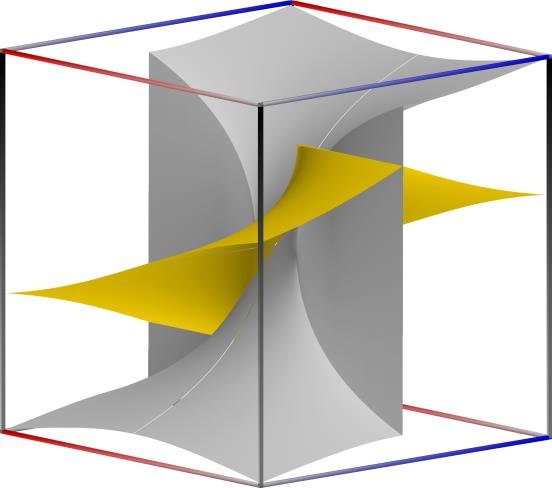
\includegraphics[height=8cm, width=8cm]{Charts/jpg/CplxAsinhBoth.jpg} }}%
	\qquad
	\subfloat[Magnitude and phase (color-coded), $z_{\text{min}}=0$. Camera angles are $\theta = 35\degree$ and $\phi = -112\degree$.]{{\includegraphics[height=8cm, width=8cm]{Charts/jpg/CplxAsinhMag.jpg} }}%
	\caption[Complex Inverse Hyperbolic Sine]{Surface plots of $z = \text{asinh}(x + iy)$, $-3 \leq x \leq 3$ (blue axis), $-2 \pi \leq y \leq 2\pi$ (red axis), $z_{\text{min}} \leq z \leq 10$ (black axis). $z$ values are truncated at $\pm 10$. There is a branch cut along the negative real axis. Orthographic camera. See section \ref{Graphics: Surface plots of complex functions} for more information about charts for complex functions.} 
	\label{fig:Complex Inverse Hyperbolic Sine}%
\end{figure}




\newpage
\subsection{\texorpdfstring{$\text{Inverse Hyperbolic Cosine: acosh}(z)$}{acosh}}

\begin{mpFunctionsExtract}
	\mpFunctionOne
	{acosh? mpNum? the inverse complex hyperbolic cosine of $z$}
	{z? mpNum? A complex number.}
\end{mpFunctionsExtract}

\vspace{0.3cm}
The function \textsf{cplxACosh$(z)$} returns the inverse complex hyperbolic cosine of $z$: 
\begin{equation}
	\text{arccosh}(z) = \pm i \text{ arccos}(z),
\end{equation}
where $\text{arccos}(z)$ is defined in section \ref{inverse complex cosine}

Computes the inverse hyperbolic cosine of $x$, $\cosh^{-1}(x)=\log(x+\sqrt{x+1}\sqrt{x-1})$.

\begin{figure}[ht]%
	\centering
	\subfloat[Real ("silver") and imaginary ("gold") component, $z_{\text{min}}=-10$. Camera angles are $\theta = 135\degree$ and $\phi = -12\degree$.]{{\includegraphics[height=8cm, width=8cm]{Charts/jpg/CplxAcoshBoth.jpg} }}%
	\qquad
	\subfloat[Magnitude and phase (color-coded), $z_{\text{min}}=0$. Camera angles are $\theta = 35\degree$ and $\phi = -112\degree$.]{{\includegraphics[height=8cm, width=8cm]{Charts/jpg/CplxAcoshMag.jpg} }}%
	\caption[Complex Inverse Hyperbolic Cosine]{Surface plots of $z = \text{acosh}(x + iy)$, $-3 \leq x \leq 3$ (blue axis), $-2 \pi \leq y \leq 2\pi$ (red axis), $z_{\text{min}} \leq z \leq 10$ (black axis). $z$ values are truncated at $\pm 10$. There is a branch cut along the negative real axis. Orthographic camera. See section \ref{Graphics: Surface plots of complex functions} for more information about charts for complex functions.} 
	\label{fig:Complex Inverse Hyperbolic Cosine}%
\end{figure}


\newpage
\subsection{\texorpdfstring{$\text{Inverse Hyperbolic Tangent: atanh}(z)$}{atanh}}

\begin{mpFunctionsExtract}
	\mpFunctionOne
	{atanh? mpNum? the inverse complex hyperbolic tangent of $z$}
	{z? mpNum? A complex number.}
\end{mpFunctionsExtract}

\vspace{0.3cm}
The function \textsf{cplxATanh$(z)$} returns the inverse complex hyperbolic tangent of $z$: 
\begin{equation}
	\text{arctanh}(z) = -i \text{ arctan}(z),
\end{equation}
where $\text{arctan}(z)$ is defined in section \ref{inverse complex tangent}

Computes the inverse hyperbolic tangent of $x$, $\tanh^{-1}(x)=\tfrac{1}{2} (\log(1+x) - \log(1+x))$.


\begin{figure}[ht]%
	\centering
	\subfloat[Real ("silver") and imaginary ("gold") component, $z_{\text{min}}=-10$. Camera angles are $\theta = 135\degree$ and $\phi = -12\degree$.]{{\includegraphics[height=8cm, width=8cm]{Charts/jpg/CplxAtanhBoth.jpg} }}%
	\qquad
	\subfloat[Magnitude and phase (color-coded), $z_{\text{min}}=0$. Camera angles are $\theta = 35\degree$ and $\phi = -112\degree$.]{{\includegraphics[height=8cm, width=8cm]{Charts/jpg/CplxAtanhMag.jpg} }}%
	\caption[Complex Inverse Hyperbolic Tangent]{Surface plots of $z = \text{atanh}(x + iy)$, $-3 \leq x \leq 3$ (blue axis), $-2 \pi \leq y \leq 2\pi$ (red axis), $z_{\text{min}} \leq z \leq 10$ (black axis). $z$ values are truncated at $\pm 10$. There is a branch cut along the negative real axis. Orthographic camera. See section \ref{Graphics: Surface plots of complex functions} for more information about charts for complex functions.} 
	\label{fig:Complex Inverse Hyperbolic Tangent}%
\end{figure}



\newpage
\subsection{\texorpdfstring{$\text{Inverse Hyperbolic Cotangent: acoth}(z)$}{acoth}}
\label{inverse complex hyperbolic cotangent}

\begin{mpFunctionsExtract}
	\mpFunctionOne
	{acoth? mpNum? the inverse complex hyperbolic cotangent of $z$}
	{z? mpNum? A complex number.}
\end{mpFunctionsExtract}

\vspace{0.3cm}
The function \textsf{cplxACoth$(z)$} returns the inverse complex hyperbolic cotangent of $z$: 
\begin{equation}
	\text{arctanh}(z) = i \text{ arctan}(iz),
\end{equation}
where $\text{arctan}(z)$ is defined in section \ref{inverse complex cotangent}



Computes the inverse hyperbolic cotangent of $x$, $\text{coth}^{-1}(x) = \tanh^{-1}(1/x)$

\begin{figure}[ht]%
	\centering
	\subfloat[Real ("silver") and imaginary ("gold") component, $z_{\text{min}}=-10$. Camera angles are $\theta = 135\degree$ and $\phi = -12\degree$.]{{\includegraphics[height=8cm, width=8cm]{Charts/jpg/CplxAcothBoth.jpg} }}%
	\qquad
	\subfloat[Magnitude and phase (color-coded), $z_{\text{min}}=0$. Camera angles are $\theta = 35\degree$ and $\phi = -112\degree$.]{{\includegraphics[height=8cm, width=8cm]{Charts/jpg/CplxAcothMag.jpg} }}%
	\caption[Complex Inverse Hyperbolic Cotangent]{Surface plots of $z = \text{acoth}(x + iy)$, $-3 \leq x \leq 3$ (blue axis), $-2 \pi \leq y \leq 2\pi$ (red axis), $z_{\text{min}} \leq z \leq 10$ (black axis). $z$ values are truncated at $\pm 10$. There is a branch cut along the negative real axis. Orthographic camera. See section \ref{Graphics: Surface plots of complex functions} for more information about charts for complex functions.} 
	\label{fig:Complex Inverse Hyperbolic Cotangent}%
\end{figure}



\subsection{asech(x)}
Computes the inverse hyperbolic secant of $x$, $\text{sech}^{-1}(x) = \cosh^{-1}(1/x)$



\subsection{acsch(x)}
Computes the inverse hyperbolic cosecant of $x$, $\text{csch}^{-1}(x) = \sinh^{-1}(1/x)$





\chapter{Linear Algebra}

\section{Norms}
Sometimes you need to know how 'large' a matrix or vector is. Due to their multidimensional nature it is not possible to compare them, but there are several functions to map a matrix or a vector to a positive real number, the so called norms.

\vpara
\begin{mpFunctionsExtract}
	\mpFunctionTwo
	{norm? mpNumList? the entrywise $p$-norm of an iterable x, i.e. the vector norm.}
	{Y? mpNum[]? An array of real numbers.}
	{Keywords? String?  p=2.}
\end{mpFunctionsExtract}


norm(ctx, x, p=2)
Gives the entrywise $p$-norm of an iterable x, i.e. the vector norm 

\begin{equation}
	\left( \sum_k |x_k|^p \right)^{1/p},
\end{equation}
for any given $1 \leq p \leq \infty$.

Special cases:

If x is not iterable, this just returns absmax(x).

p=1 gives the sum of absolute values.

p=2 is the standard Euclidean vector norm.

p=inf gives the magnitude of the largest element.

For x a matrix, p=2 is the Frobenius norm. For operator matrix norms, use mnorm() instead.

You can use the string 'inf' as well as float('inf') or mpf('inf') to specify the infinity norm.

\vpara
\textbf{Examples}

\lstset{language={Python}}
\begin{lstlisting}
>>> from mpFormulaPy import *
>>> mp.dps = 15; mp.pretty = False
>>> x = matrix([-10, 2, 100])
>>> norm(x, 1)
mpf('112.0')
>>> norm(x, 2)
mpf('100.5186549850325')
>>> norm(x, inf)
mpf('100.0')
\end{lstlisting}


\vspace{0.6cm}

\begin{mpFunctionsExtract}
	\mpFunctionTwo
	{mnorm? mpNumList? the matrix (operator) $p$-norm of A. Currently p=1 and p=inf are supported.}
	{A? mpNum[]? An array of real numbers.}
	{Keywords? String?  p=1.}
\end{mpFunctionsExtract}


mnorm(ctx, A, p=1)

Gives the matrix (operator) $p$-norm of A. Currently p=1 and p=inf are supported:

p=1 gives the 1-norm (maximal column sum)

p=inf gives the -norm (maximal row sum). You can use the string 'inf' as well as float('inf') or mpf('inf')

p=2 (not implemented) for a square matrix is the usual spectral matrix norm, i.e. the largest singular value.

p='f' (or 'F', 'fro', 'Frobenius', 'frobenius') gives the Frobenius norm, which is the elementwise 2-norm. The Frobenius norm is an approximation of the spectral norm and satisfies

\begin{equation}
	\frac{1}{\sqrt{\text{rank}(A)}} ||A||_F \leq ||A||_2 \leq ||A||_F.
\end{equation}

The Frobenius norm lacks some mathematical properties that might be expected of a norm.

For general elementwise $p$-norms, use norm() instead.

\vpara
\textbf{Examples}

\lstset{language={Python}}
\begin{lstlisting}
>>> from mpFormulaPy import *
>>> mp.dps = 15; mp.pretty = False
>>> A = matrix([[1, -1000], [100, 50]])
>>> mnorm(A, 1)
mpf('1050.0')
>>> mnorm(A, inf)
mpf('1001.0')
>>> mnorm(A, 'F')
mpf('1006.2310867787777')
\end{lstlisting}





\newpage
\section{Decompositions}


\begin{mpFunctionsExtract}
	\mpFunctionTwo
	{cholesky? mpNum? the Cholesky decomposition of a symmetric positive-definite matrix $A$.}
	{A? mpNum[]? A symmetric matrix.}
	{Keywords? String?  tol=None.}
\end{mpFunctionsExtract}


cholesky(ctx, A, tol=None)

Cholesky decomposition of a symmetric positive-definite matrix $A$. Returns a lower triangular matrix $L$ such that $A=L \times L^T$. More generally, for a complex Hermitian positive-definite matrix, a Cholesky decomposition satisfying $A=L \times L^H$ is returned.

\vpara
The Cholesky decomposition can be used to solve linear equation systems twice as efficiently as LU decomposition, or to test whether $A$ is positive-definite.

\vpara
The optional parameter tol determines the tolerance for verifying positive-definiteness.

\vpara
\textbf{Examples}

Cholesky decomposition of a positive-definite symmetric matrix:

\lstset{language={Python}}
\begin{lstlisting}
>>> from mpFormulaPy import *
>>> mp.dps = 25; mp.pretty = True
>>> A = eye(3) + hilbert(3)
>>> nprint(A)
[ 2.0 0.5 0.333333]
[ 0.5 1.33333 0.25]
[0.333333 0.25 1.2]
>>> L = cholesky(A)
>>> nprint(L)
[ 1.41421 0.0 0.0]
[0.353553 1.09924 0.0]
[0.235702 0.15162 1.05899]
>>> chop(A - L*L.T)
[0.0 0.0 0.0]
[0.0 0.0 0.0]
[0.0 0.0 0.0]
\end{lstlisting}

Cholesky decomposition of a Hermitian matrix:

\lstset{language={Python}}
\begin{lstlisting}
>>> A = eye(3) + matrix([[0,0.25j,-0.5j],[-0.25j,0,0],[0.5j,0,0]]
>>> L = cholesky(A)
>>> nprint(L)
[ 1.0 0.0 0.0]
[(0.0 - 0.25j) (0.968246 + 0.0j) 0.0]
[ (0.0 + 0.5j) (0.129099 + 0.0j) (0.856349 + 0.0j)]
>>> chop(A - L*L.H)
[0.0 0.0 0.0]
[0.0 0.0 0.0]
[0.0 0.0 0.0]
\end{lstlisting}

Attempted Cholesky decomposition of a matrix that is not positive definite:

\lstset{language={Python}}
\begin{lstlisting}
>>> A = -eye(3) + hilbert(3)
>>> L = cholesky(A)
Traceback (most recent call last):
...
ValueError: matrix is not positive-definite
\end{lstlisting}




\newpage
\section{Linear Equations}


\begin{mpFunctionsExtract}
	\mpFunctionThree
	{lu\_solve? mpNum? solves a linear equation system using a LU decomposition.}
	{A? mpNum[]? A symmetric matrix.}
	{b? mpNum[]? A symmetric matrix.}	
	{Keywords? String?  tol=None.}
\end{mpFunctionsExtract}


You can for example solve the linear equation system using a LU decomposition:

\lstset{language={Python}}
\begin{lstlisting}
x + 2*y = -10
3*x + 4*y = 10
\end{lstlisting}

using lu\_solve:

\lstset{language={Python}}
\begin{lstlisting}
>>> A = matrix([[1, 2], [3, 4]])
>>> b = matrix([-10, 10])
>>> x = lu_solve(A, b)
>>> x
matrix(
[['30.0'],
['-20.0']])
\end{lstlisting}


\begin{mpFunctionsExtract}
	\mpFunctionFour
	{residual? mpNum? the residual  $||Ax-b||$.}
	{A? mpNum[]? A square matrix.}
	{b? mpNum[]? A vector.}
	{x? mpNum[]? A vector.}		
	{Keywords? String?  tol=None.}
\end{mpFunctionsExtract}


Calculates the residual  $||Ax-b||$:

\lstset{language={Python}}
\begin{lstlisting}
>>> residual(A, x, b)
matrix(
[['3.46944695195361e-18'],
['3.46944695195361e-18']])
>>> str(eps)
'2.22044604925031e-16'
\end{lstlisting}

As you can see, the solution is quite accurate. The error is caused by the inaccuracy of the internal floating point arithmetic. Though, it is even smaller than the current machine epsilon, which basically means you can trust the result.

If you need more speed, use NumPy, or use fp instead mp matrices and methods:

\lstset{language={Python}}
\begin{lstlisting}
>>> A = fp.matrix([[1, 2], [3, 4]])
>>> b = fp.matrix([-10, 10])
>>> fp.lu_solve(A, b)
matrix(
[['30.0'],
['-20.0']])
\end{lstlisting}

lu\_solve accepts overdetermined systems. It is usually not possible to solve such systems, so the residual is minimized instead. Internally this is done using Cholesky decomposition to compute a least squares approximation. This means that that lu\_solve will square the errors. If you cannot afford this, use qr\_solve instead. It is twice as slow but more accurate, and it calculates the residual automatically.



\newpage
\section{Matrix Factorization}

\begin{mpFunctionsExtract}
	\mpFunctionTwo
	{lu? mpNum? an explicit LU factorization of a matrix, returning P, L, U}
	{A? mpNum[]? A square matrix.}
	{Keywords? String?  tol=None.}
\end{mpFunctionsExtract}


The function lu computes an explicit LU factorization of a matrix:

\lstset{language={Python}}
\begin{lstlisting}
>>> P, L, U = lu(matrix([[0,2,3],[4,5,6],[7,8,9]]))
>>> print P
[0.0 0.0 1.0]
[1.0 0.0 0.0]
[0.0 1.0 0.0]
>>> print L
[ 1.0 0.0 0.0]
[ 0.0 1.0 0.0]
[0.571428571428571 0.214285714285714 1.0]
>>> print U
[7.0 8.0 9.0]
[0.0 2.0 3.0]
[0.0 0.0 0.214285714285714]
>>> print P.T*L*U
[0.0 2.0 3.0]
[4.0 5.0 6.0]
[7.0 8.0 9.0]
\end{lstlisting}




\begin{mpFunctionsExtract}
	\mpFunctionTwo
	{qr? mpNum? an explicit QR factorization of a matrix, returning Q, R}
	{A? mpNum[]? A square matrix.}
	{Keywords? String?  tol=None.}
\end{mpFunctionsExtract}

\vpara
Examples:

\lstset{language={Python}}
\begin{lstlisting}
>>> A = matrix([[1, 2], [3, 4], [1, 1]])
>>> Q, R = qr(A)
>>> print Q
[-0.301511344577764 0.861640436855329 0.408248290463863]
[-0.904534033733291 -0.123091490979333 -0.408248290463863]
[-0.301511344577764 -0.492365963917331 0.816496580927726]
>>> print R
[-3.3166247903554 -4.52267016866645]
[ 0.0 0.738548945875996]
[ 0.0 0.0]
>>> print Q * R
[1.0 2.0]
[3.0 4.0]
[1.0 1.0]
>>> print chop(Q.T * Q)
[1.0 0.0 0.0]
[0.0 1.0 0.0]
[0.0 0.0 1.0]
\end{lstlisting}



